%#BIBTEX /usr/texbin/bibtex main
\documentclass[10pt,twocolumn,letterpaper]{article}

\usepackage{iccv}
\usepackage{times}
\usepackage{epsfig}
\usepackage{graphicx}
\usepackage{amsmath}
\usepackage{nccmath}
\usepackage{amssymb}
\usepackage{algorithm}
\usepackage{algorithmic}
\usepackage{tabularx}
\usepackage{comment}
\usepackage{wrapfig}
\usepackage{enumitem}
%\usepackage{algpseudocode}


\usepackage[utf8]{inputenc}
\usepackage[english]{babel}
\usepackage{amsthm}
 
\newtheorem{theorem}{Theorem}[section]
%\newtheorem{corollary}{Corollary}[theorem]
\newtheorem{lemma}[theorem]{Lemma}


\newcommand{\Tref}[1]{Table~\ref{#1}}
\newcommand{\Eref}[1]{Eq.~(\ref{#1})}
\newcommand{\Fref}[1]{Fig.~\ref{#1}}
\newcommand{\Sref}[1]{Section~\ref{#1}}
\newcommand{\Aref}[1]{Algorithm~\ref{#1}}
\newcommand{\argmax}{\mathop{\rm arg~max}\limits}
\newcommand{\argmin}{\mathop{\rm arg~min}\limits}

\newcommand{\mysubsubsection}[1]{\vspace{0.1cm} \noindent \underline{{\bf #1}}:}
\newcommand{\mysubsubsubsection}[1]{\vspace{0.1cm} \noindent {\bf #1}:}
\newcommand{\ikehata}[1]{\textcolor{blue}{ikehata:{#1}}}
\newcommand{\yasu}[1]{\textcolor{magenta}{[yasu: {#1}]}}
\newcommand{\hang}[1]{\textcolor{cyan}{[hang: {#1}]}}
%\newcommand{\ikehata}[1]{}
%\newcommand{\yasu}[1]{}
%\newcommand{\hang}[1]{}

% Include other packages here, before hyperref.

% If you comment hyperref and then uncomment it, you should delete
% egpaper.aux before re-running latex.  (Or just hit 'q' on the first latex
% run, let it finish, and you should be clear).
\usepackage[pagebackref=true,breaklinks=true,letterpaper=true,colorlinks,bookmarks=false]{hyperref}

 \iccvfinalcopy % *** Uncomment this line for the final submission

\def\iccvPaperID{745} % *** Enter the ICCV Paper ID here
\def\httilde{\mbox{\tt\raisebox{-.5ex}{\symbol{126}}}}

\ifx\pdfoptionalwaysusepdfpagebox\relax\else
\pdfoptionalwaysusepdfpagebox5
\fi


% Pages are numbered in submission mode, and unnumbered in camera-ready
\ificcvfinal\pagestyle{empty}\fi
\begin{document}


%%%%%%%% TITLE
\title{Structured Indoor Modeling\\Supplementary Material}
\author{Paper ID 745}
\maketitle
%\thispagestyle{empty}
%

%\section*{Contents}
The document provides additional experimental results, algorithmic
details, and theorem proofs, which were not included in the main paper
due to the space limitation.
%\yasu{I don't know why I cannot move the first figures to the first
%page..}

% This appendix provides details about the noise removal of the input
% point cloud, and the detailed implementation of the indoor structure
% grammer and our extensive application that have been omitted due to the
% space limit.

\section{Additional Experimental Results} \label{section:supple:results}

The section presents complete experimental results and evaluations.
Please see the caption for the explanation of each figure.

%We here describe the details of the room annotation and object
%annotation experiments.


%Figure~\ref{fig:object_recog} shows the object annotation results, which
%turn out to be much more challenging than the room annotations, even
%with the state-of-the-art object
%detectors~\cite{berkeley_object_detection_software}.

% The scene recognition
% did not work well with the panorama images, and we render $400\times
% 300$ standard perspective images with the horizontal field of view of
% $90$ degrees. The results depend on the viewing directions and we
% experimented with the four algorithms as shown in
% Table~\ref{table:scene}.  The first algorithm, for example, picks the
% panorama closest to the room center, renders six uniformly overlapping
% images, and picks the scene type with the best average score. This
% performs the worst. The best algorithm looks at all the panorama images
% that are inside the room, but uses the single rendered image in which
% the room is the most visible in the top-down view. An observation is
% that poorly positioned panoramas tend to yield incorrect results but
% with very high confidence. A rather better strategy is to use the best
% viewing direction from the best panorama.

\clearpage
\begin{figure*}[!t]
%  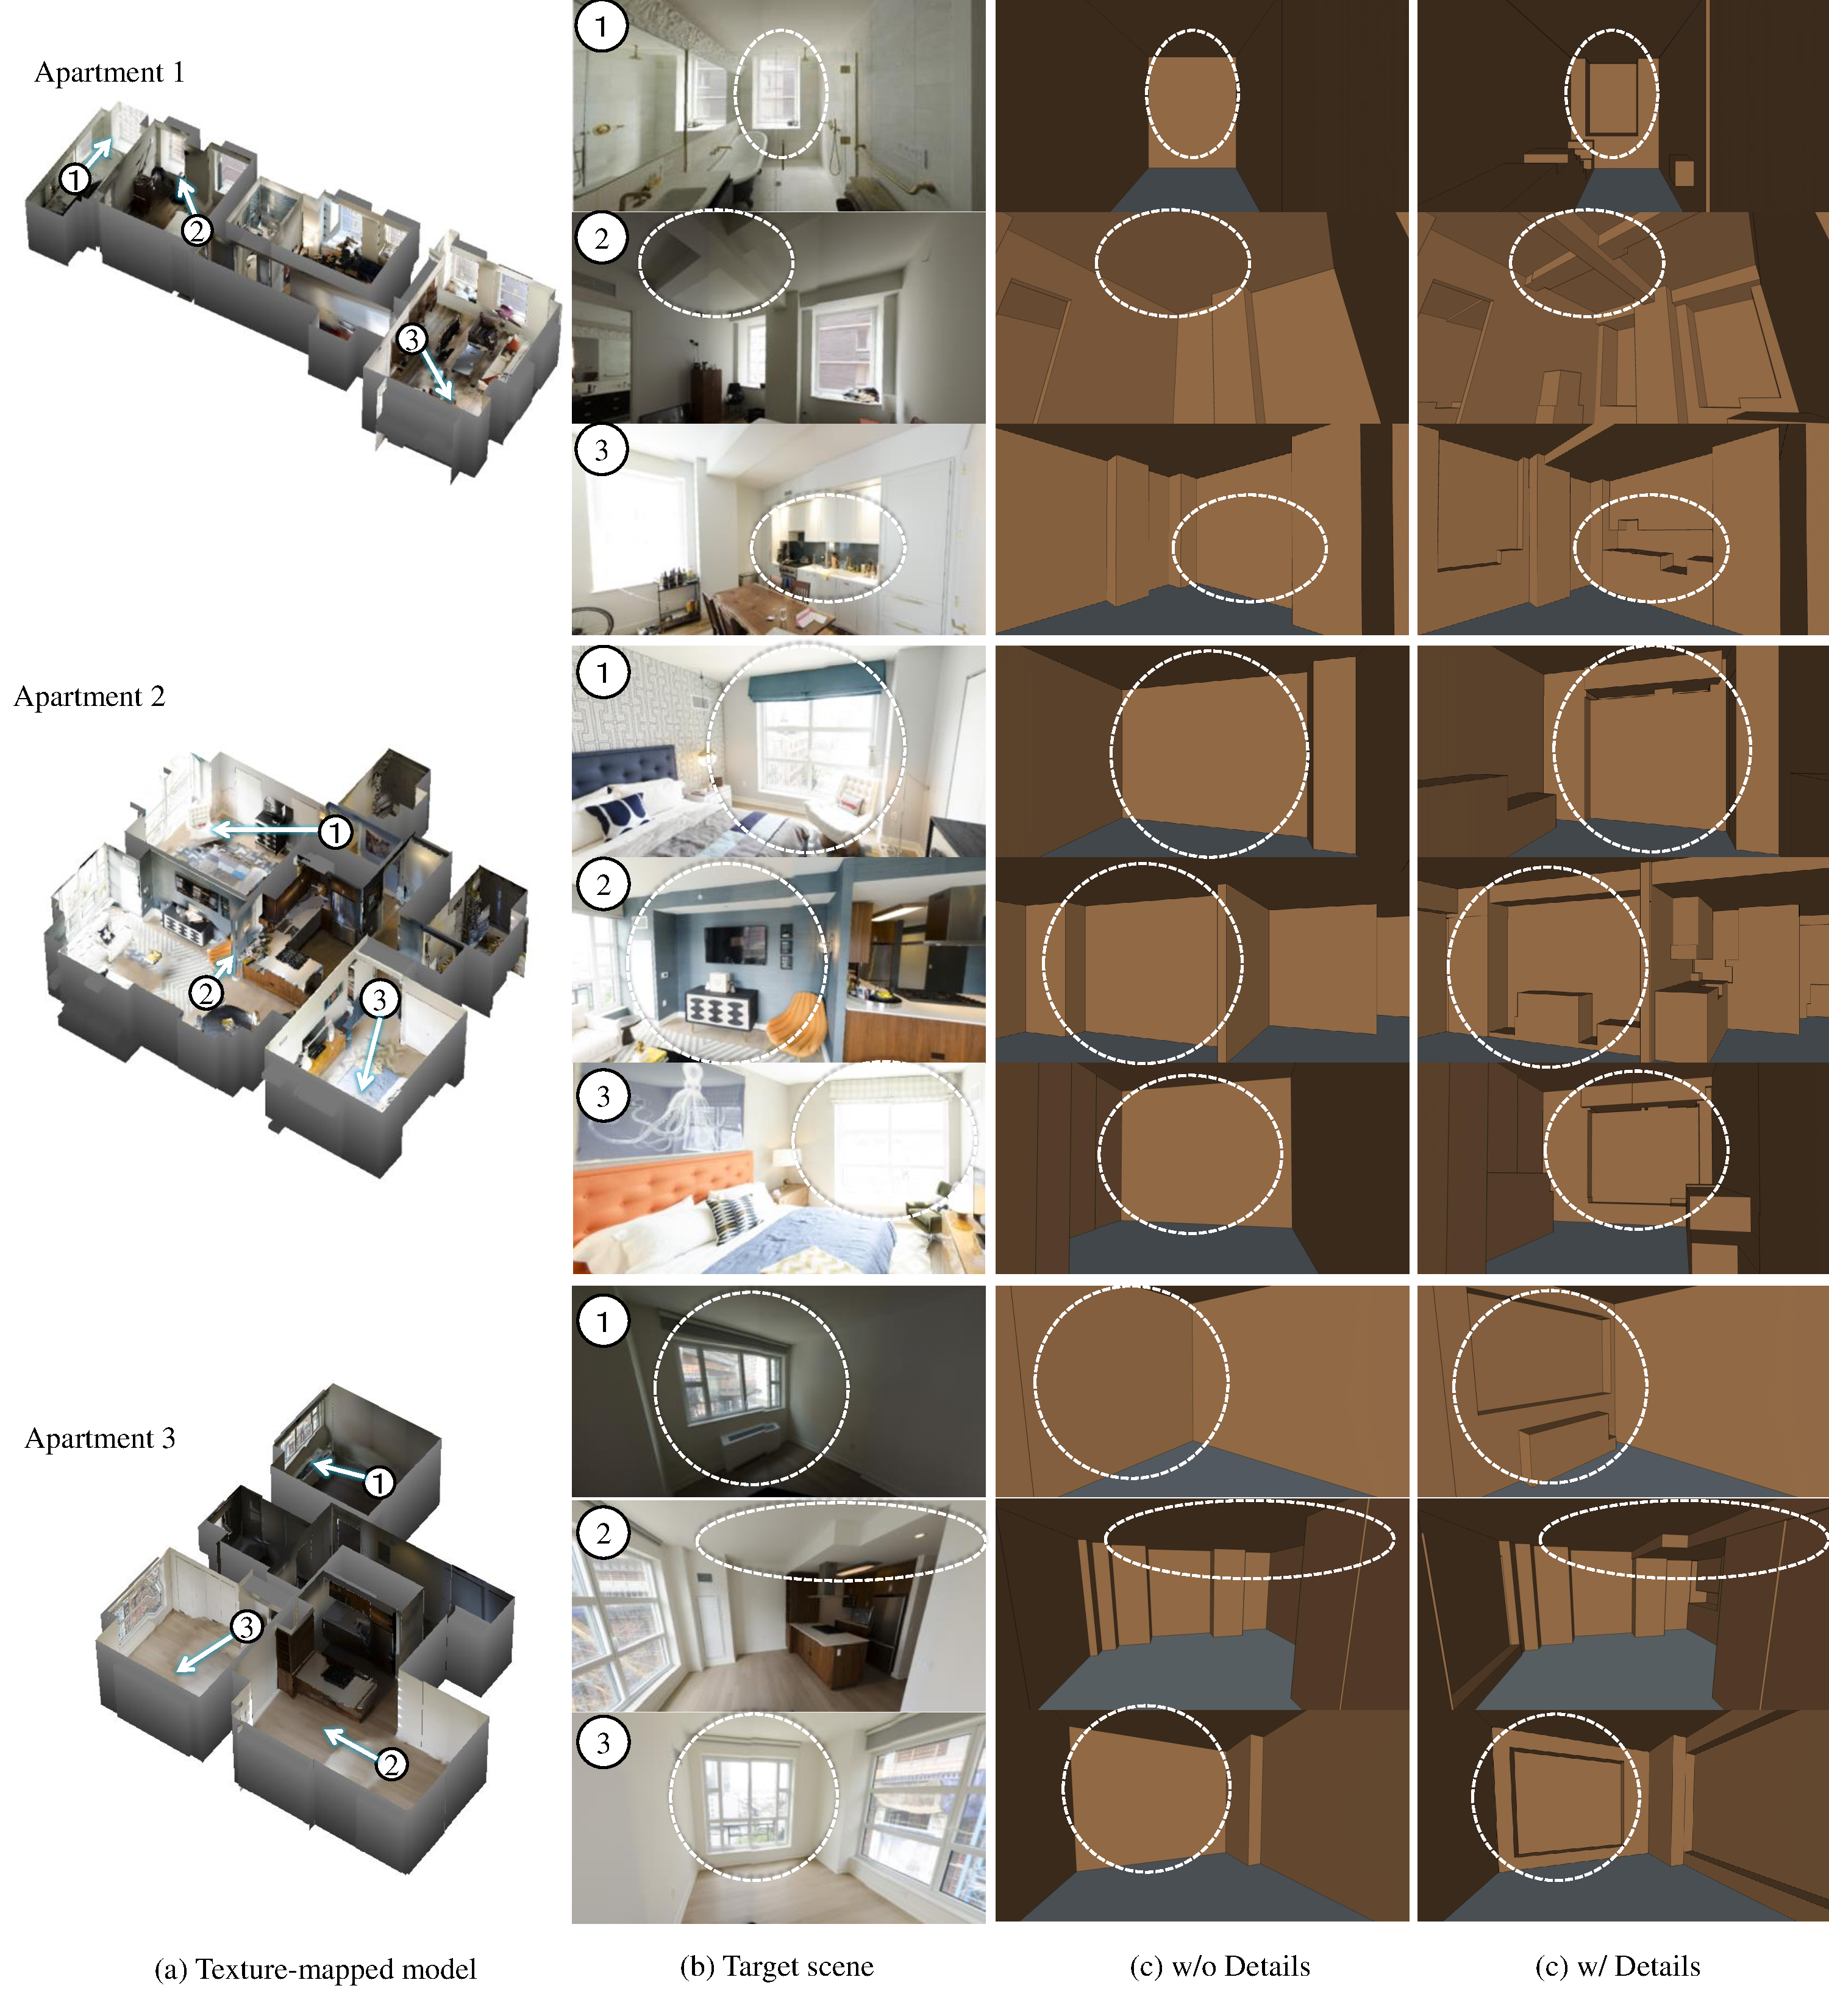
\includegraphics[width=\textwidth]{../figures/closeups1.png}
 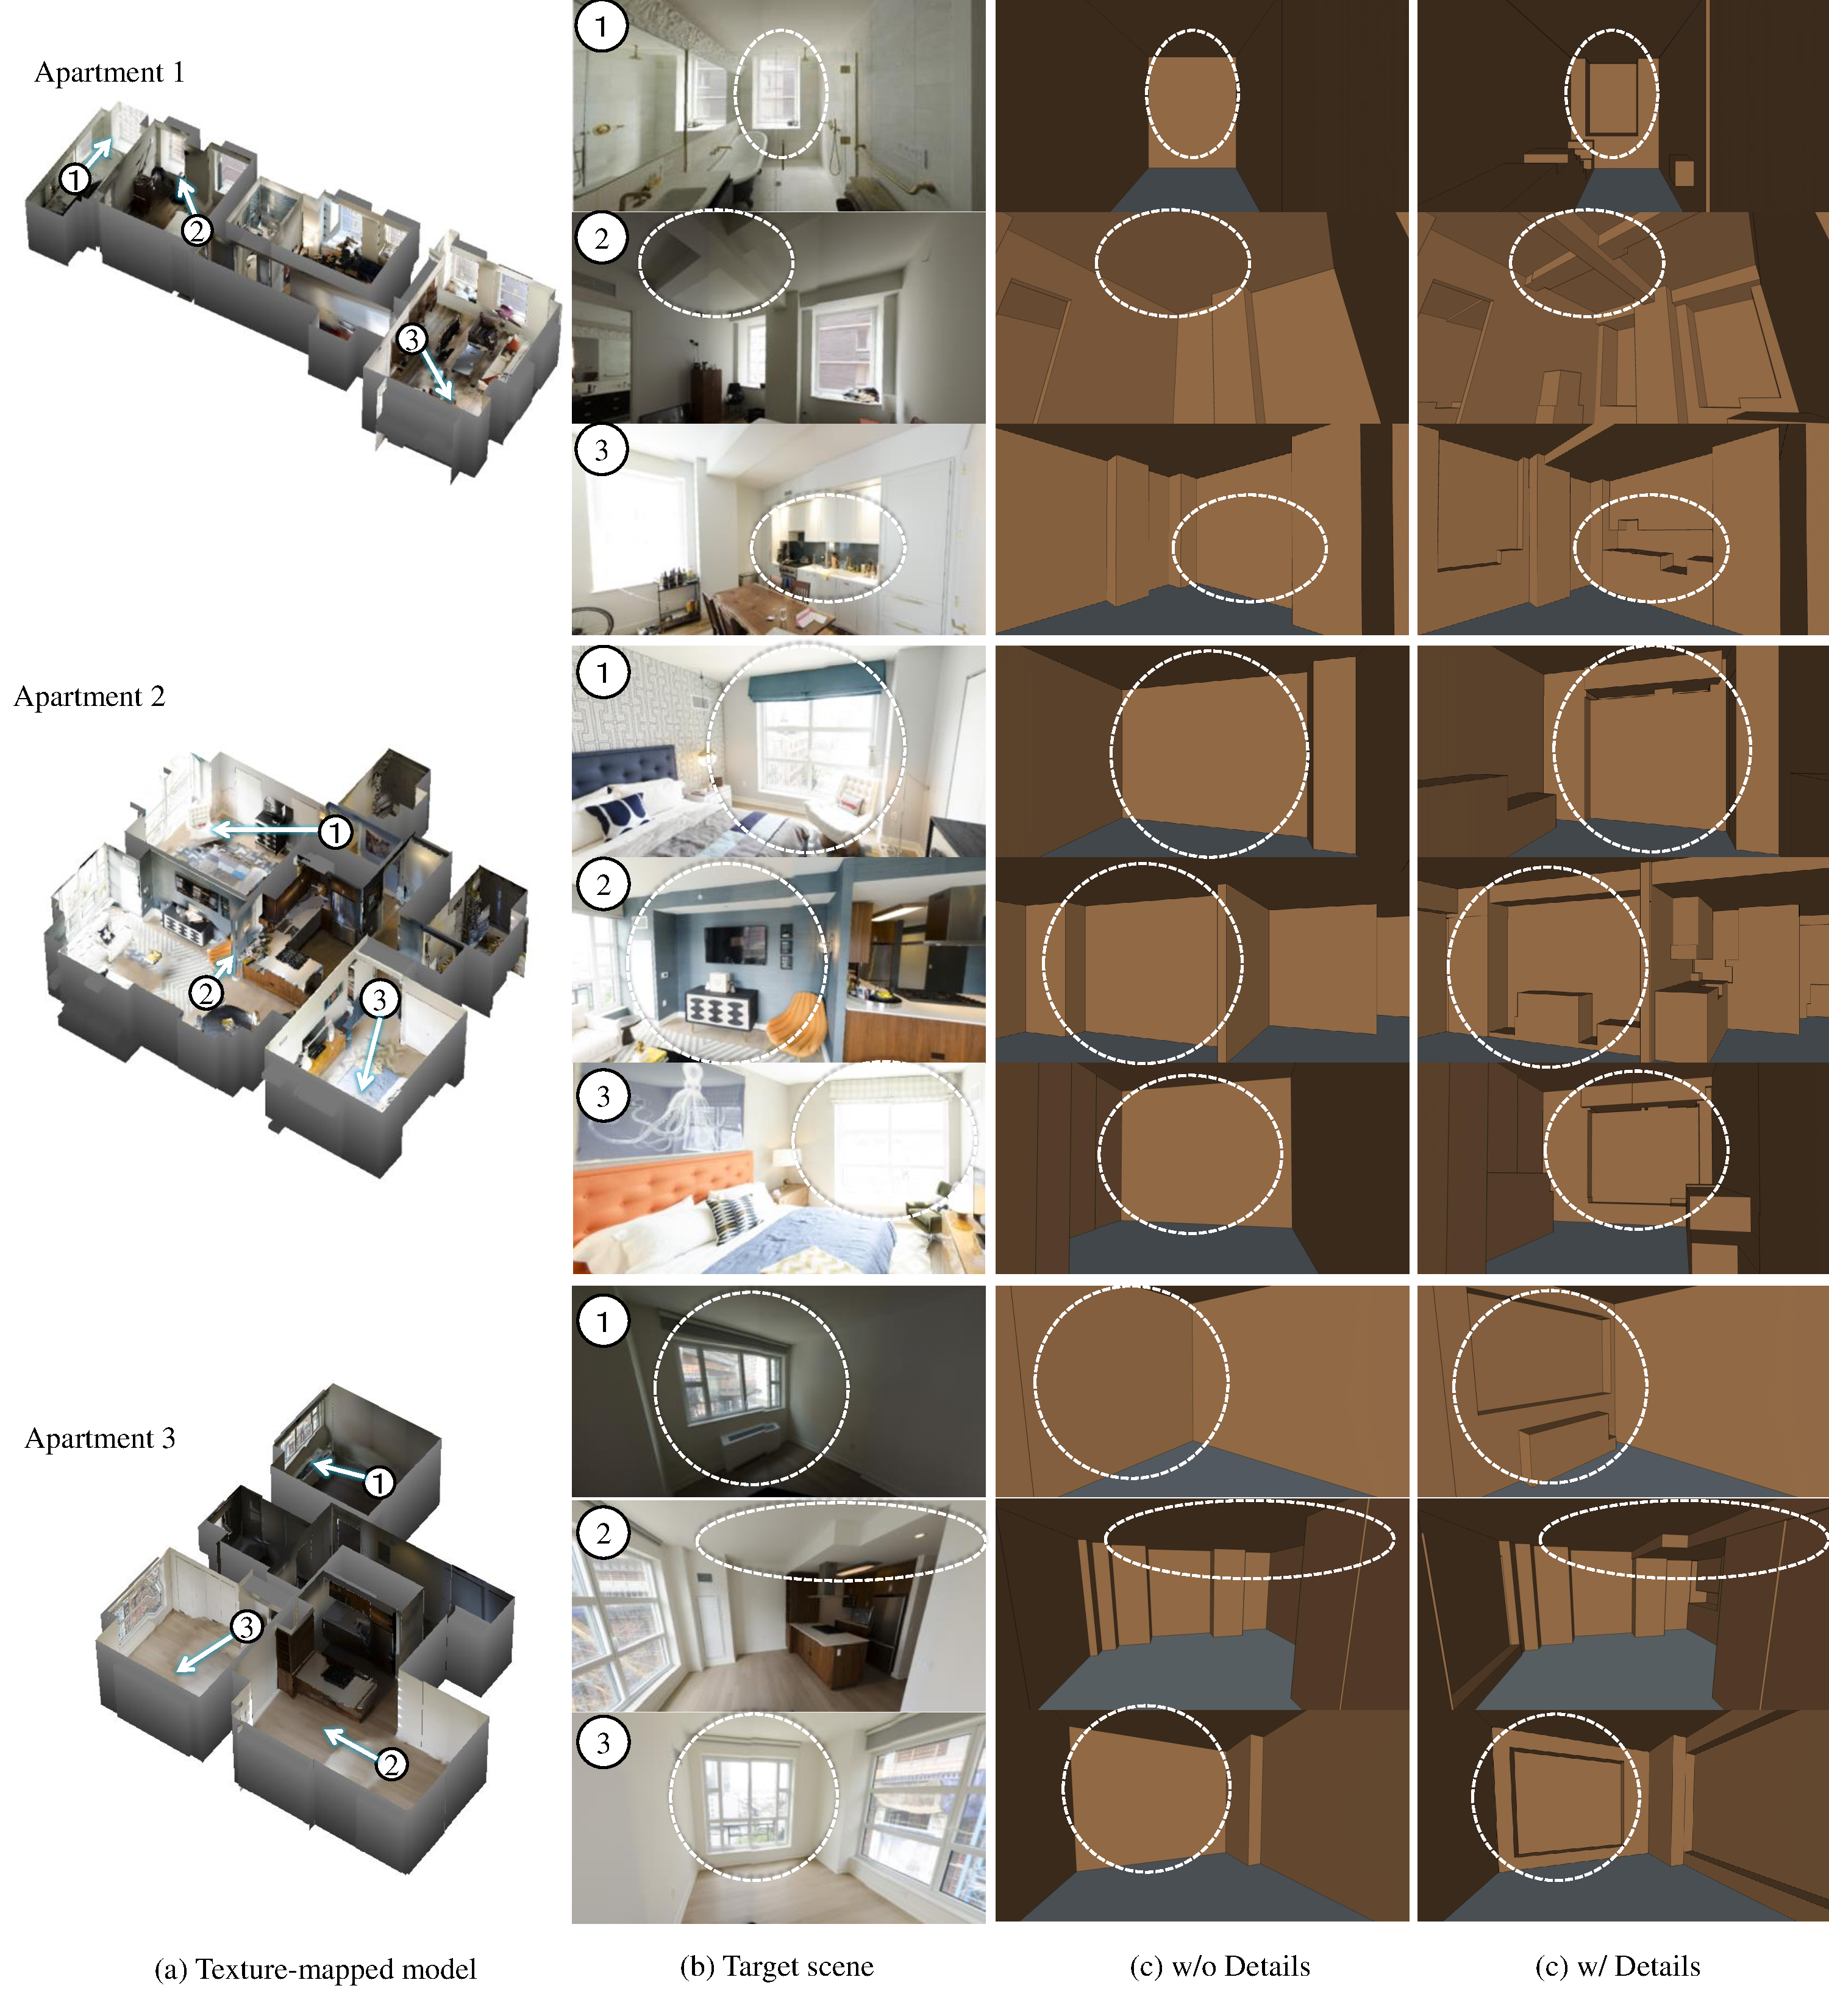
\includegraphics[width=\textwidth]{../figures/closeups1.pdf}
%		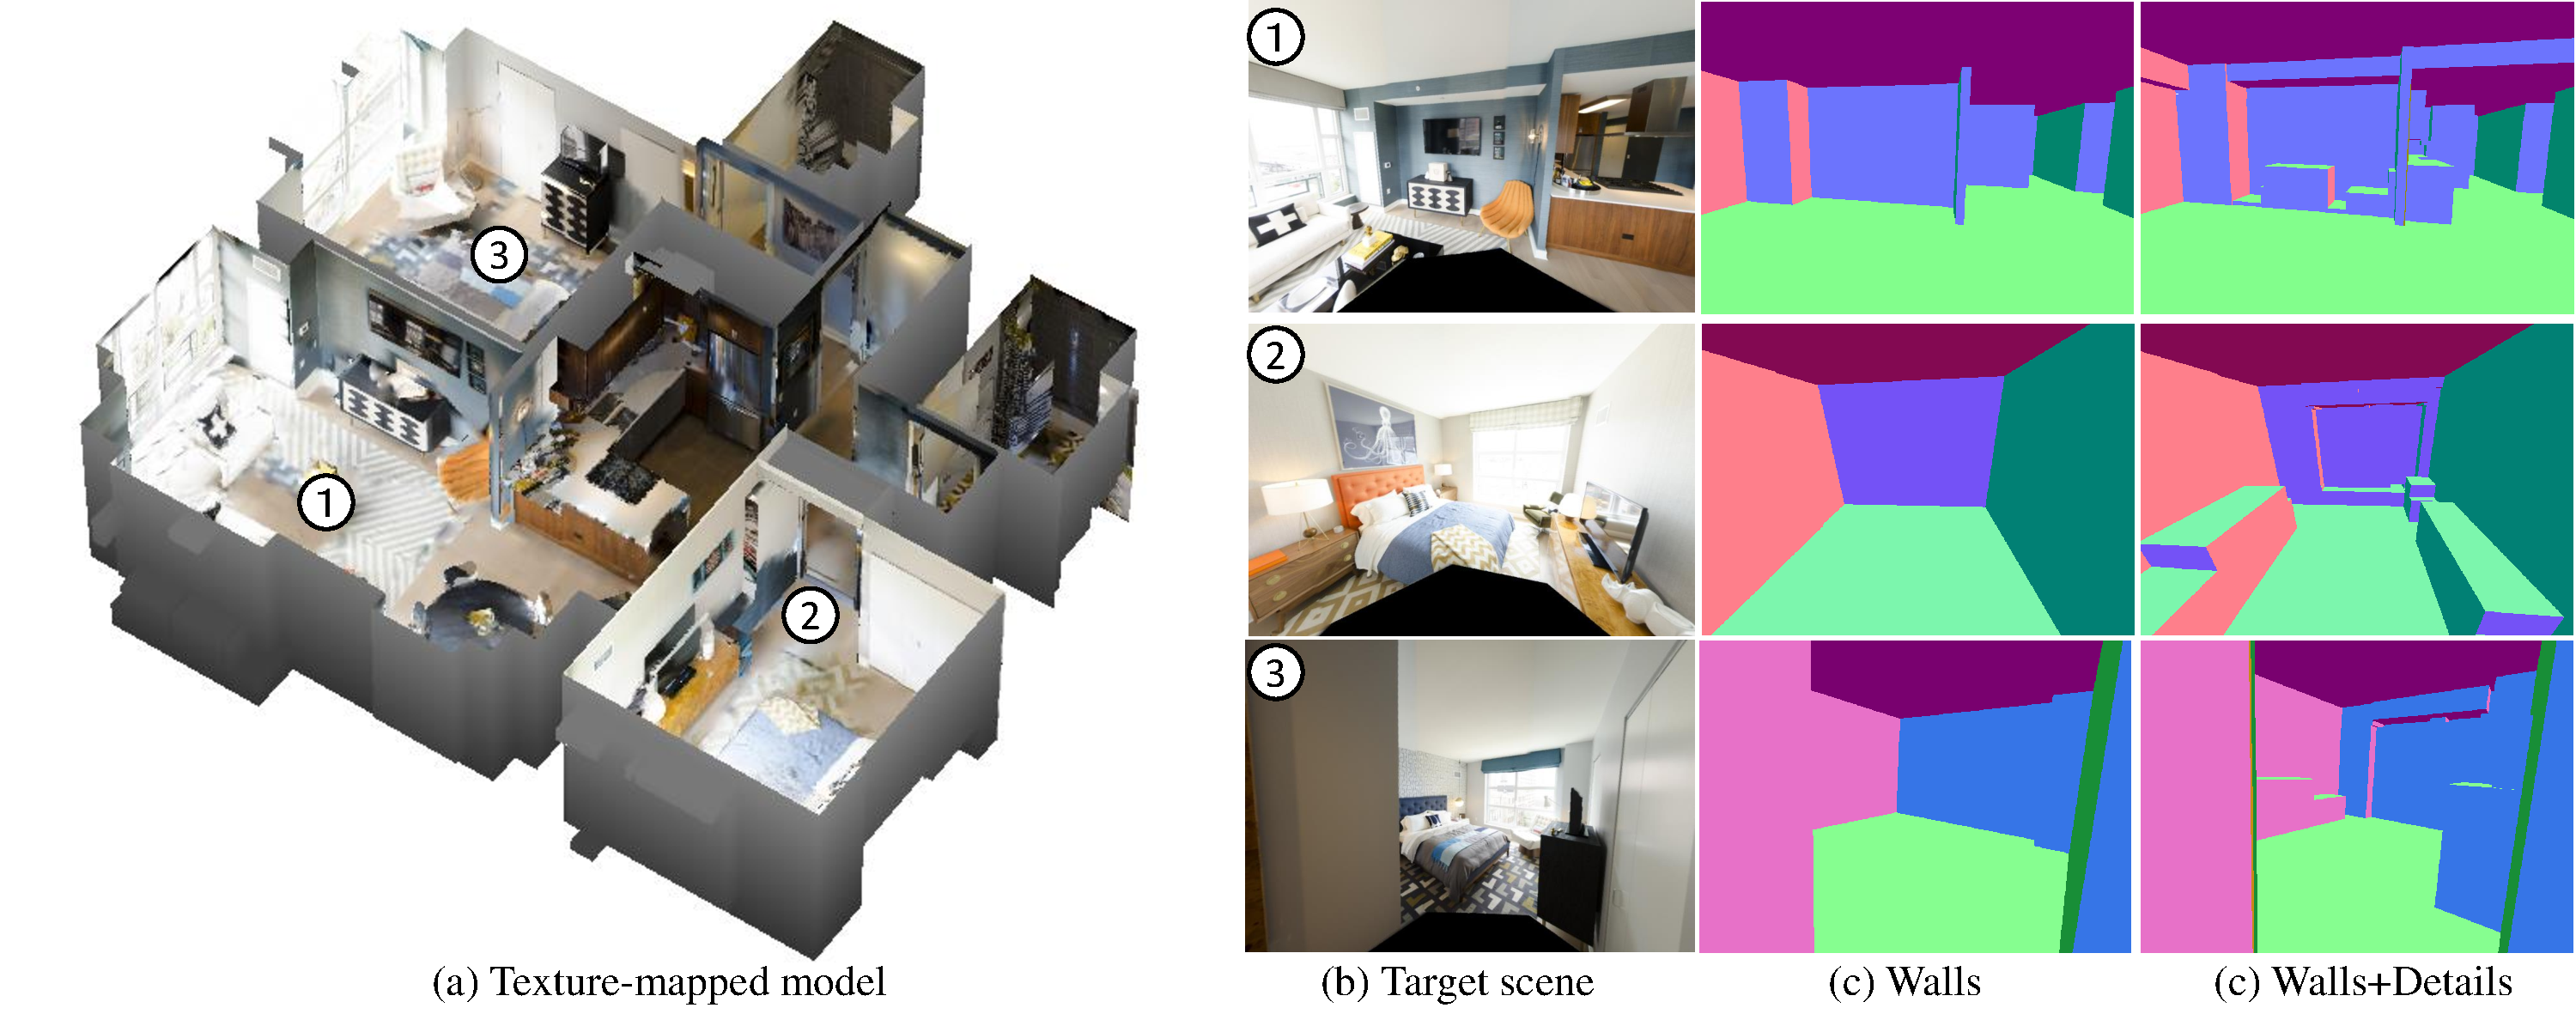
\includegraphics[width=\textwidth]{../figures/equal-sky.pdf}
%		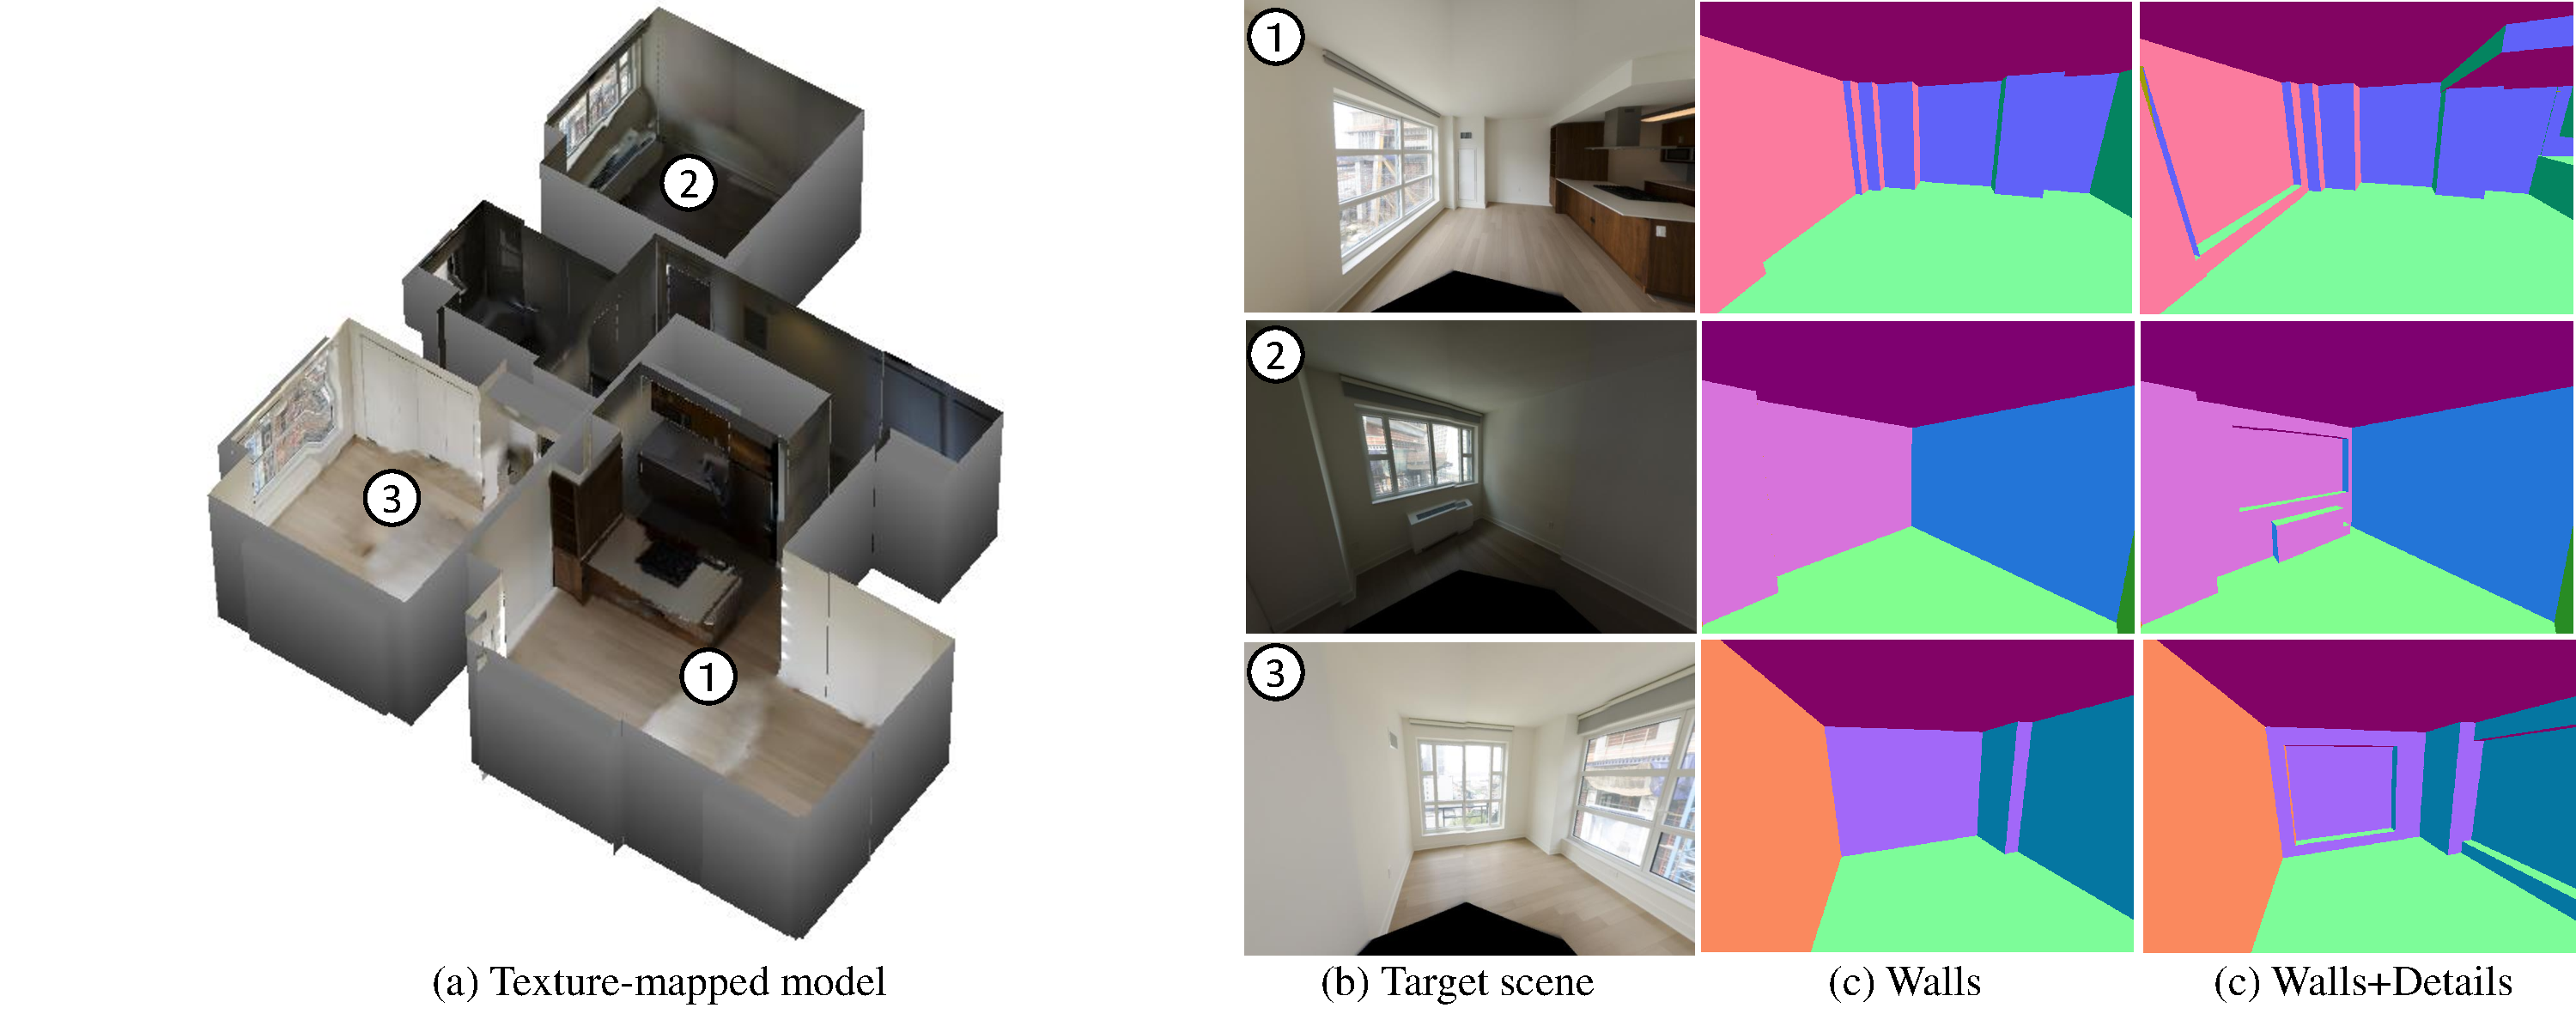
\includegraphics[width=\textwidth]{../figures/salmon-palace.pdf}
	\caption{The figure shows that our offset-map reconstruction
 algorithm is able to produce highly regularized and compact 3D
 structure. We show three examples for each dataset.}
 \label{fig:detail0}
\end{figure*}

\clearpage
\begin{figure*}[!t]
% 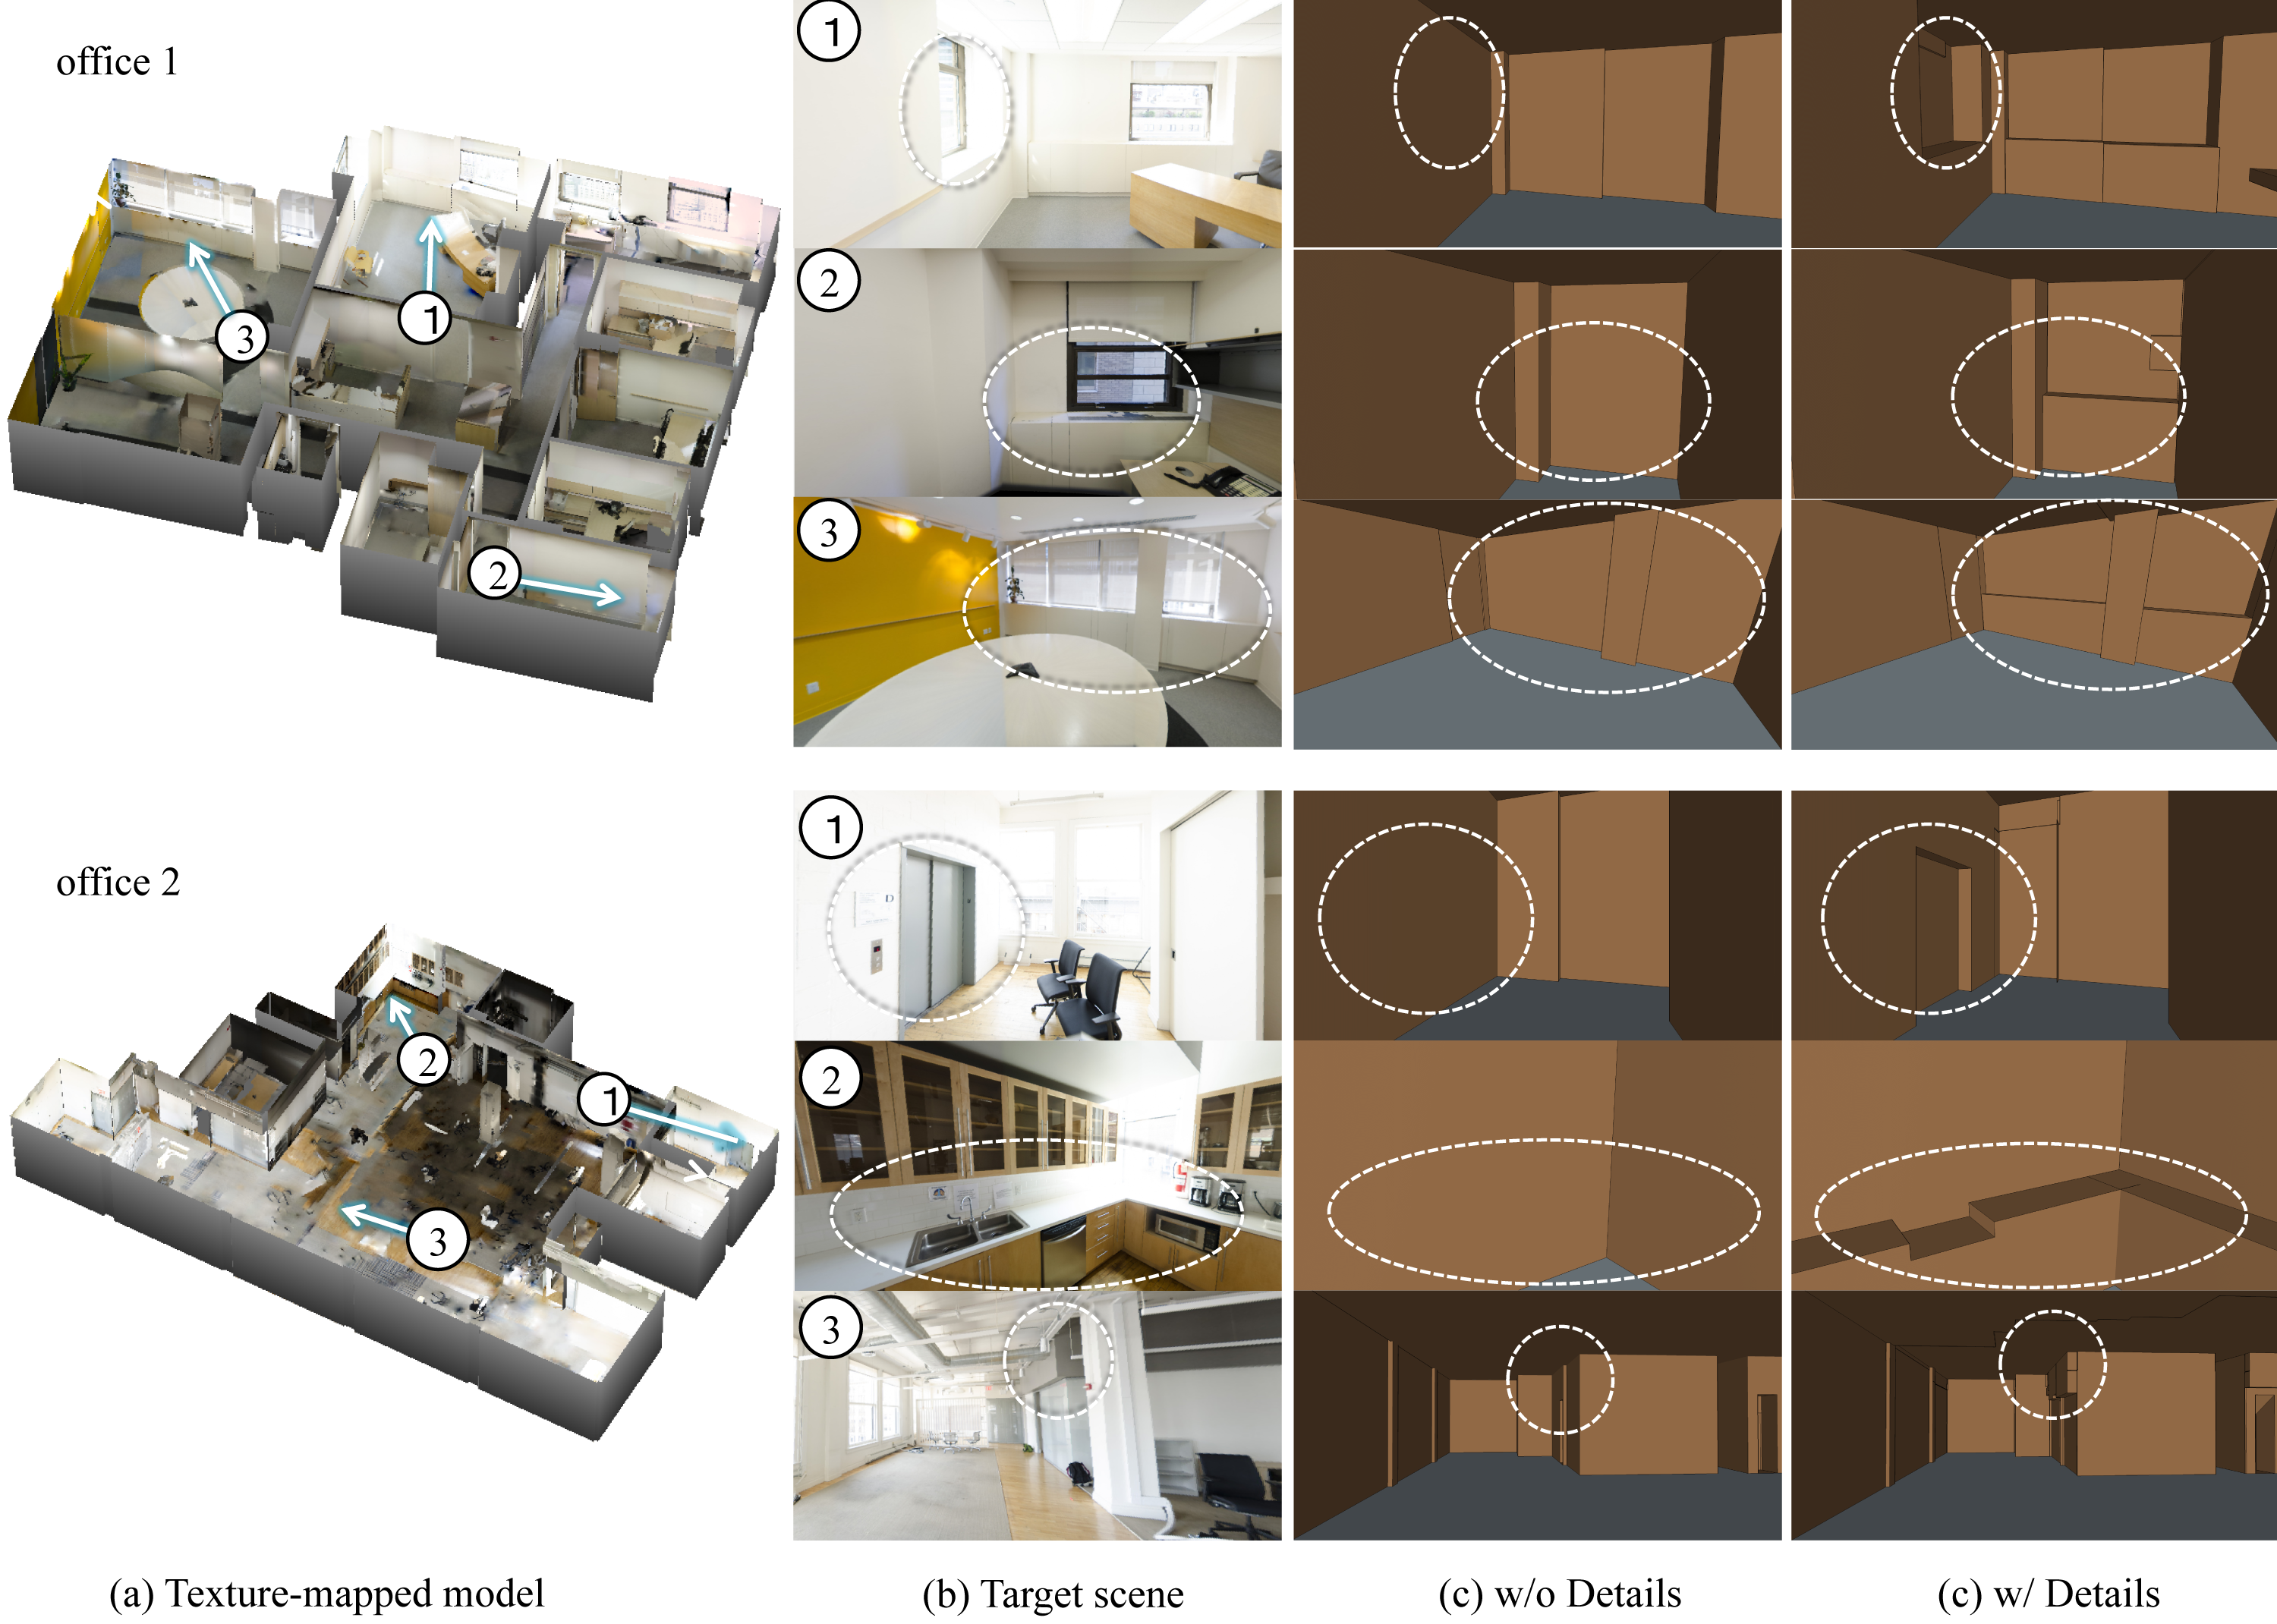
\includegraphics[width=\textwidth]{../figures/closeups2-2.png}
  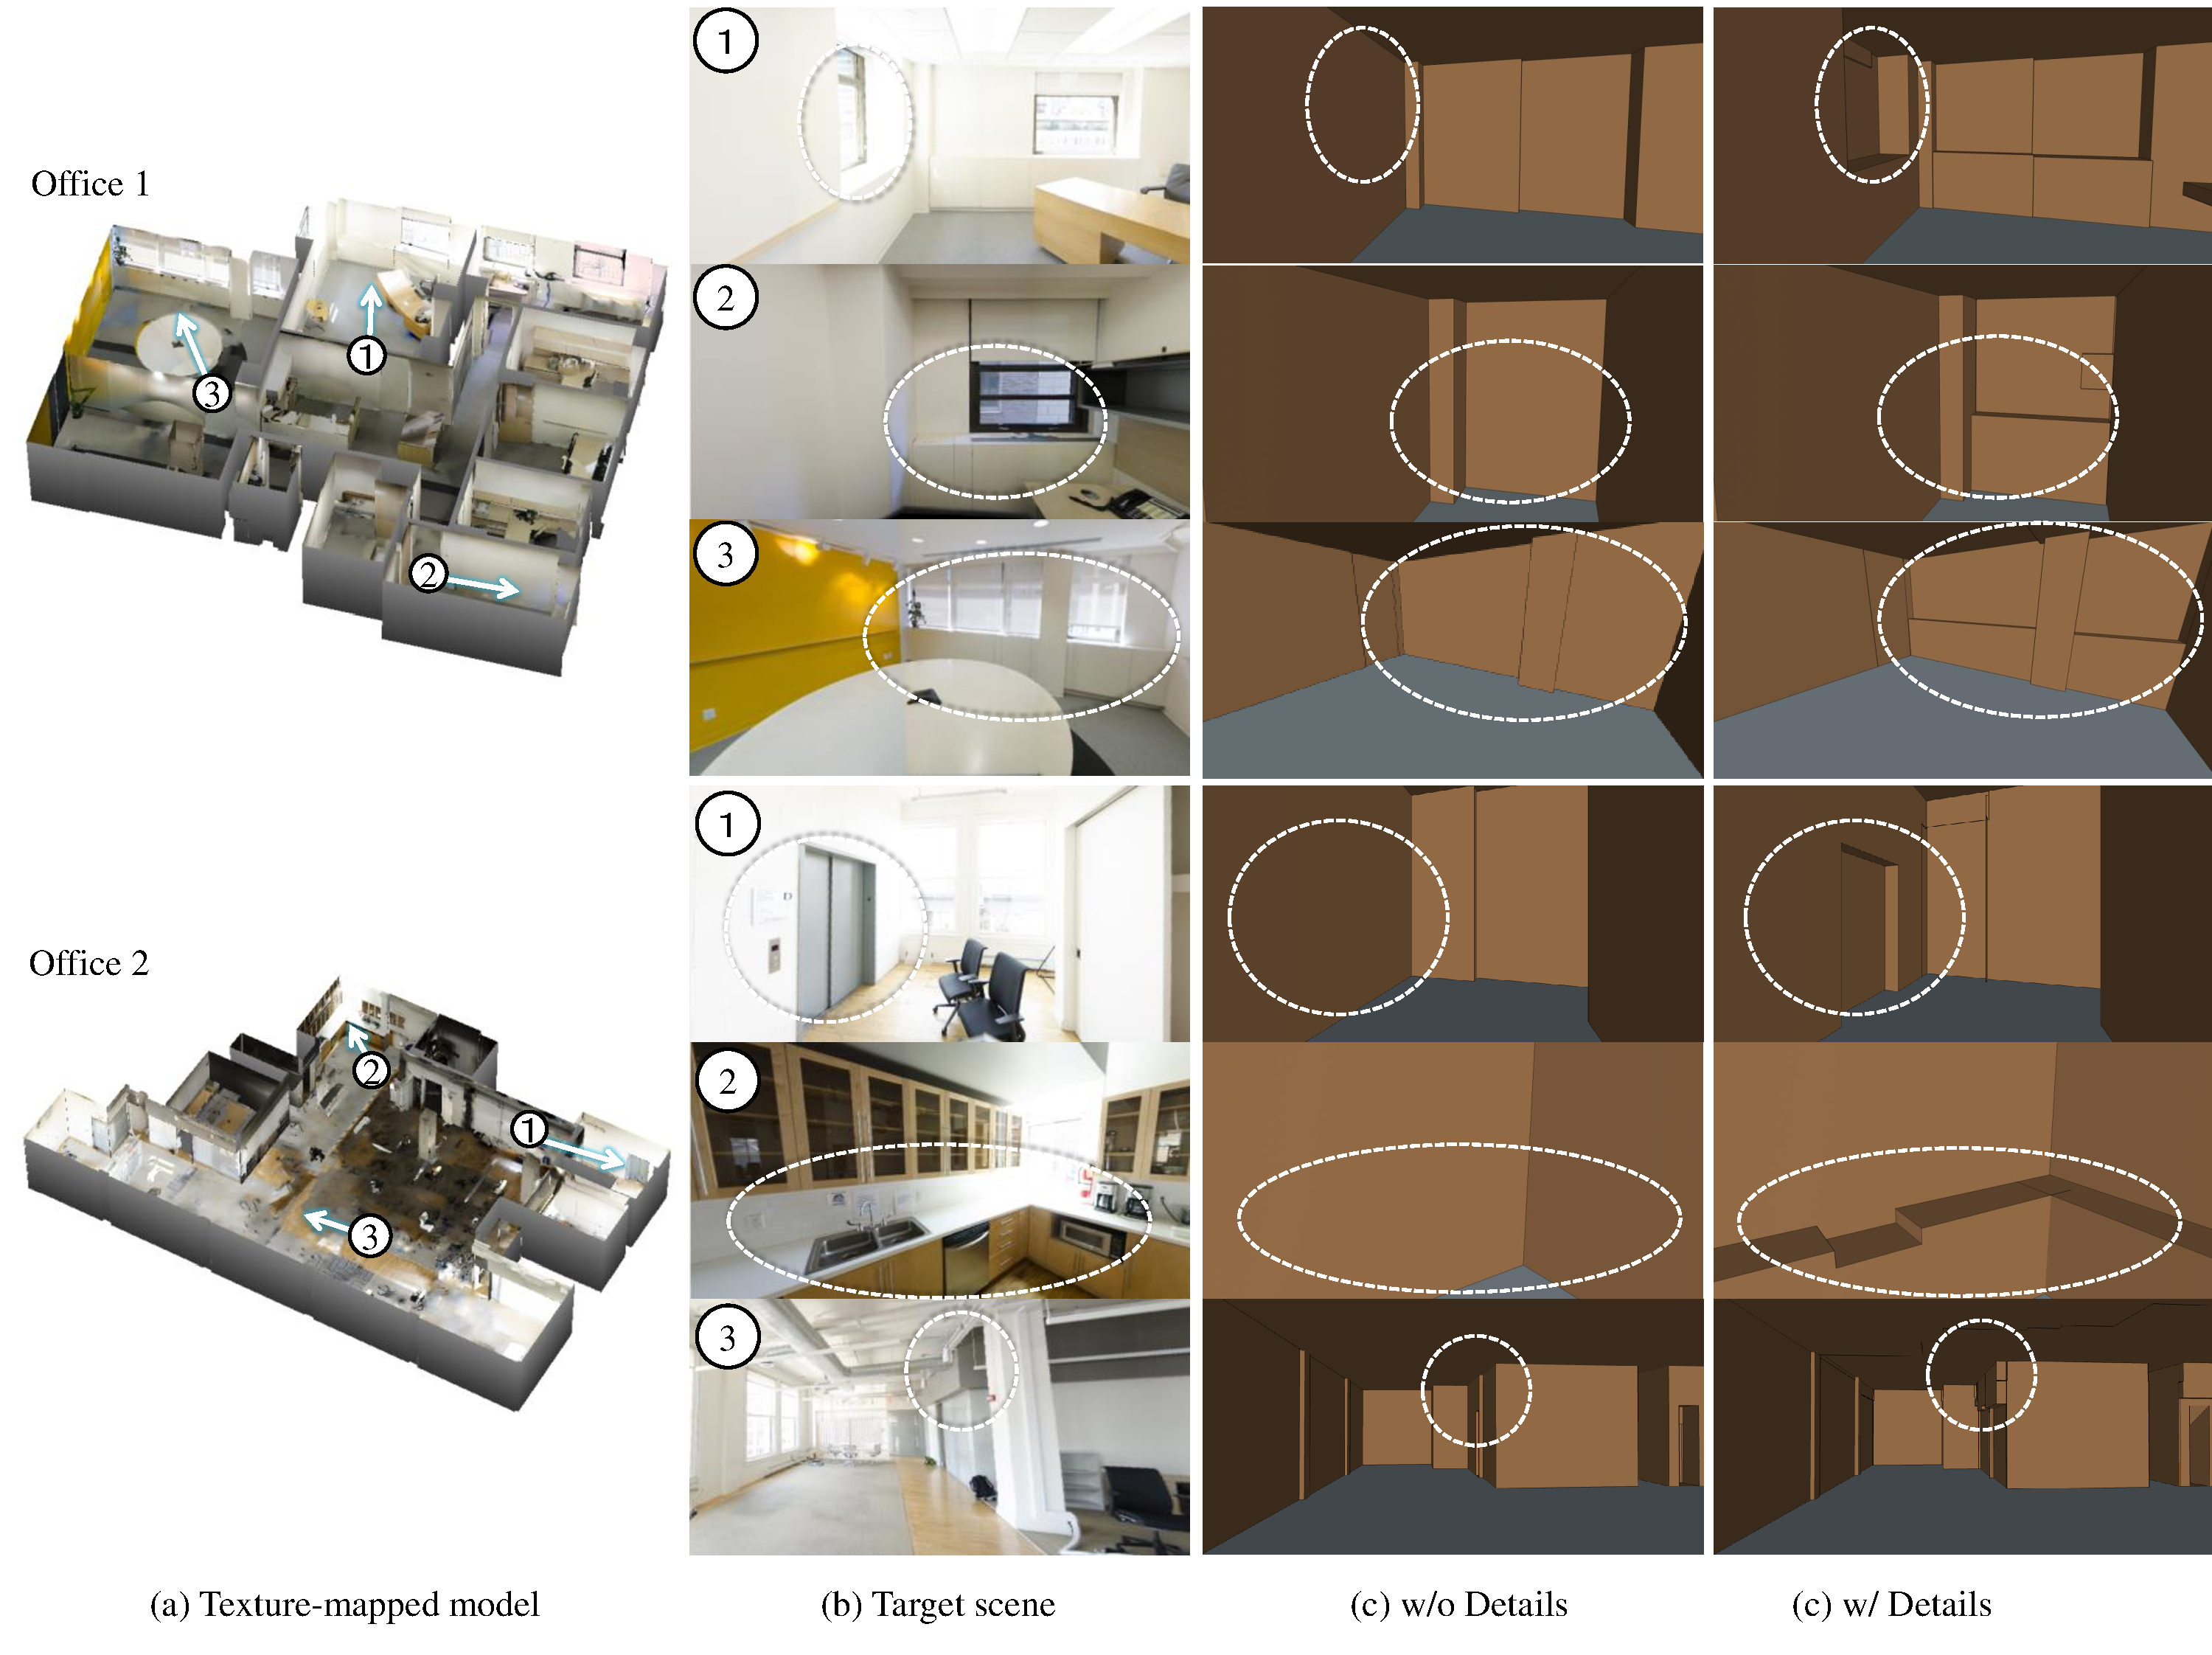
\includegraphics[width=\textwidth]{../figures/closeups2.pdf}
 \caption{Continued.}  \label{fig:detail1}
\end{figure*}

\clearpage
\begin{figure*}
 \begin{center}
%  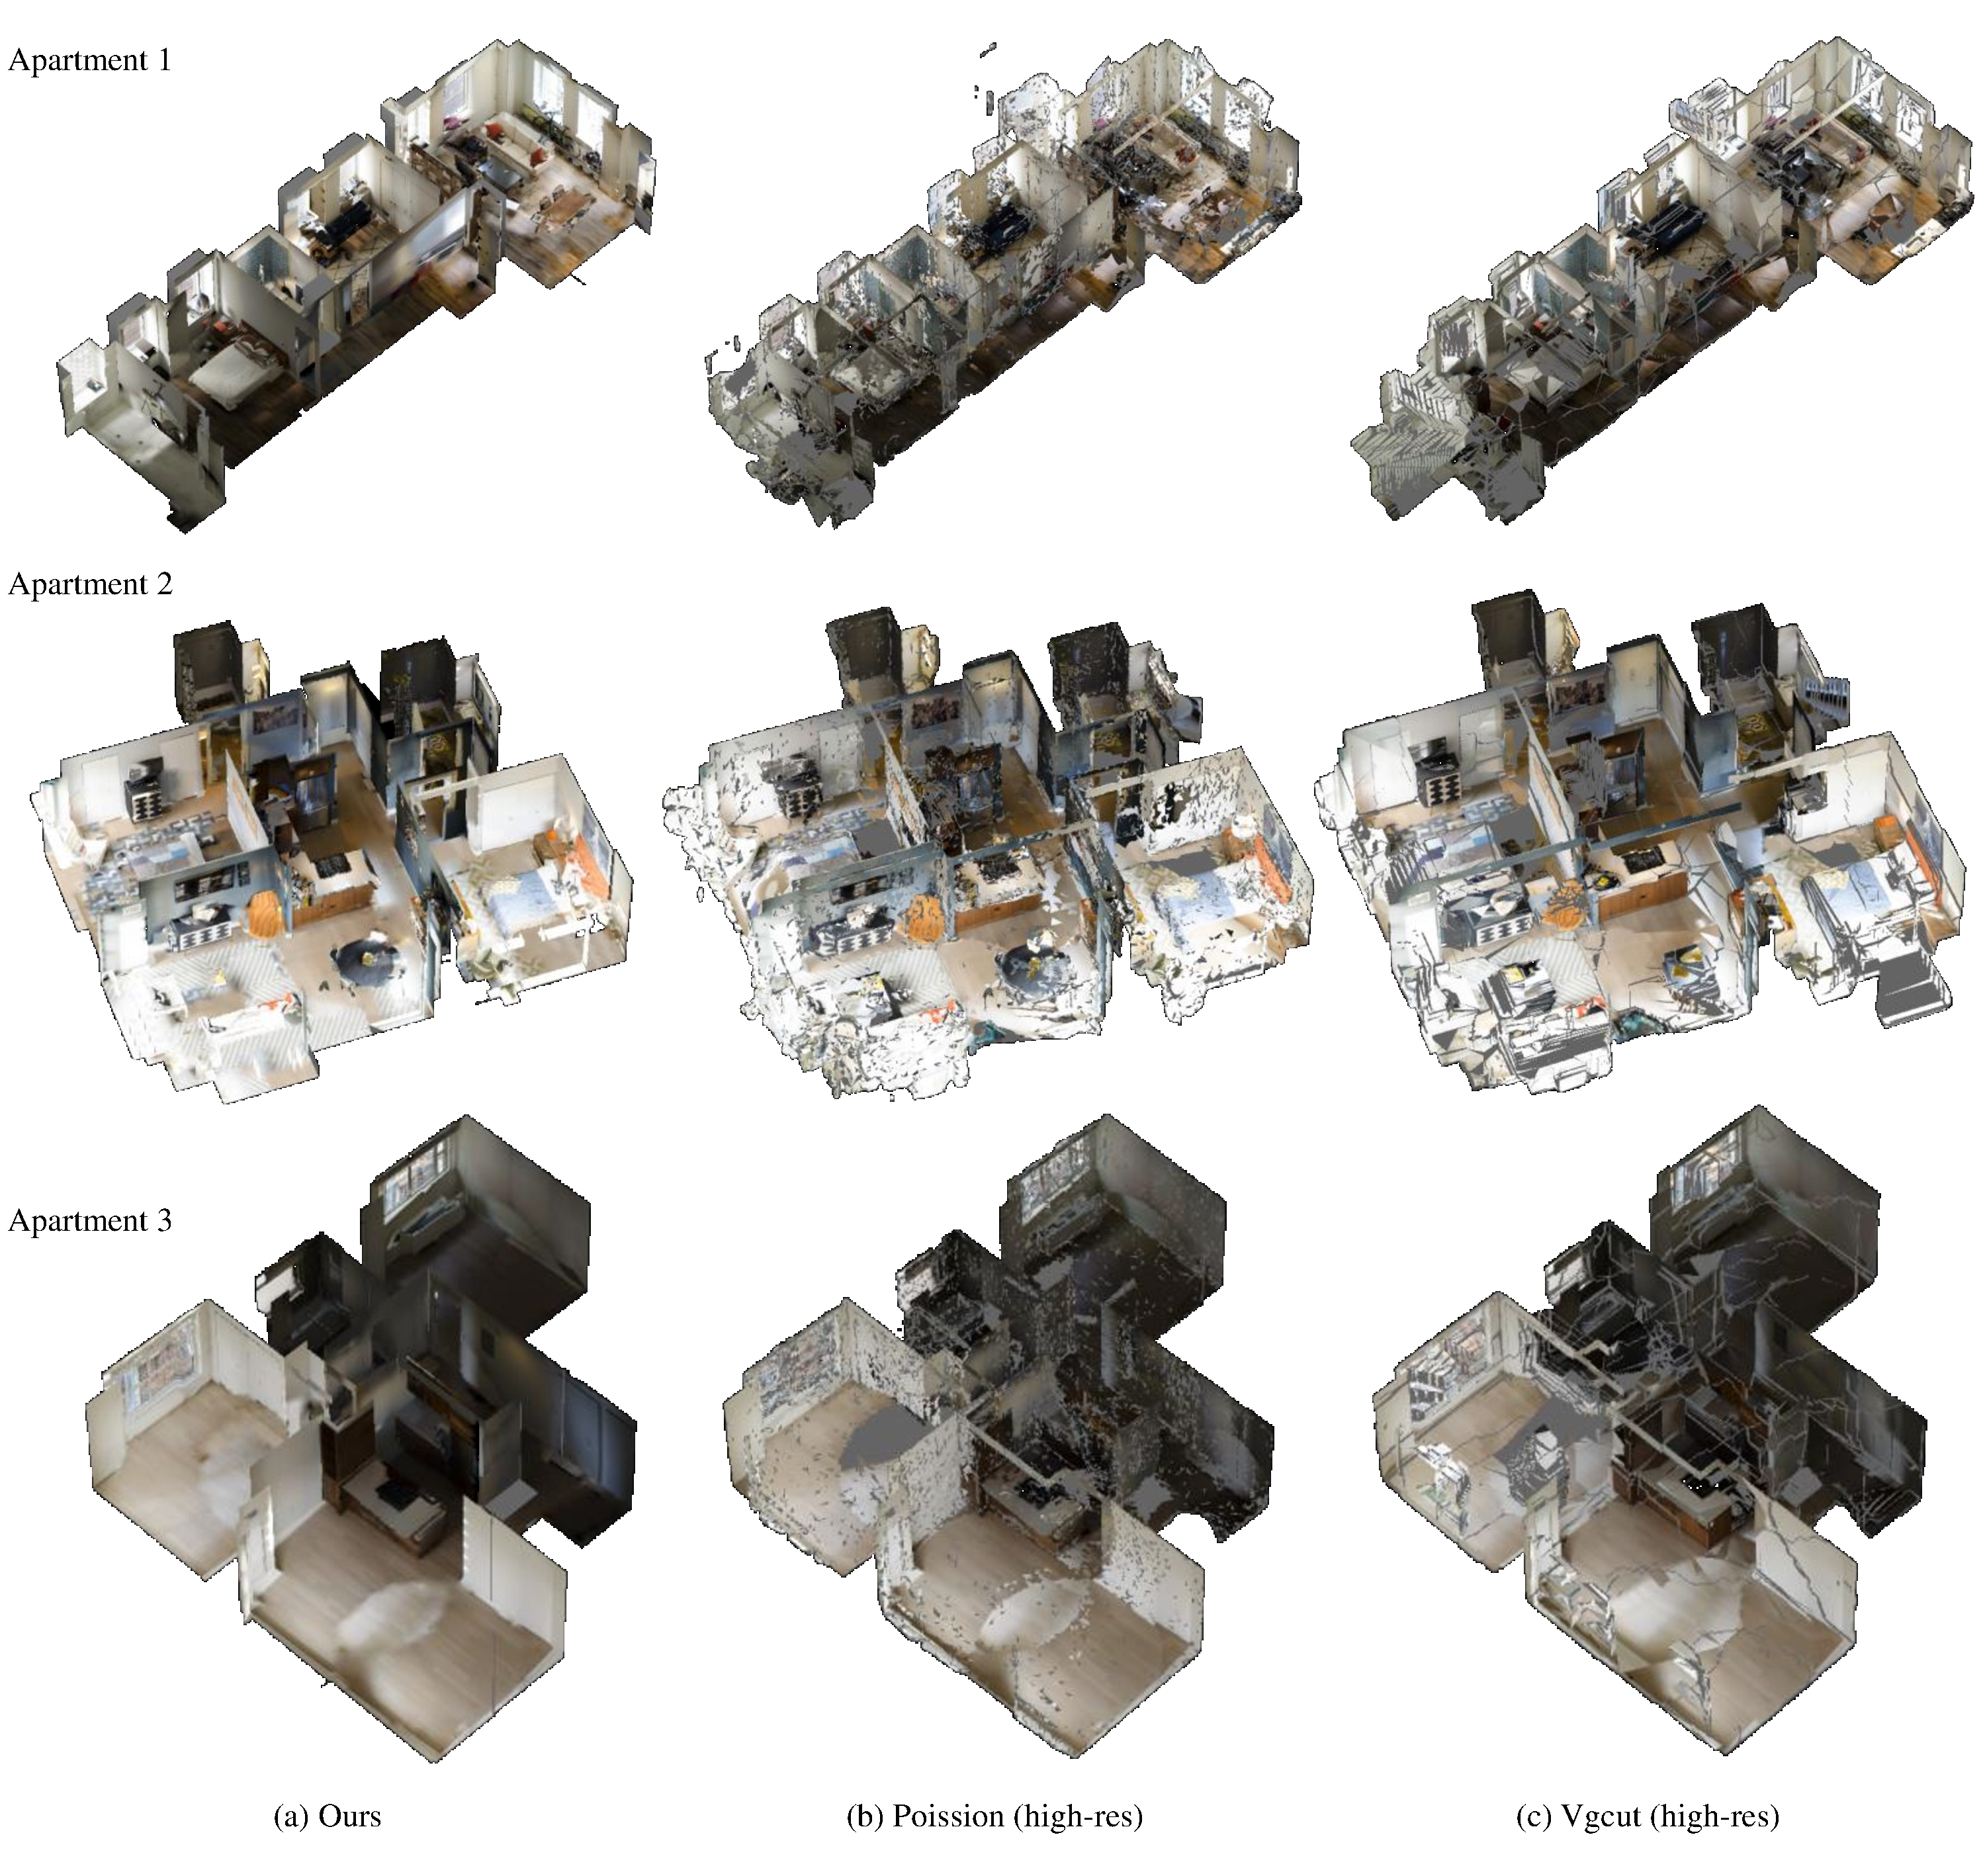
\includegraphics[width=\textwidth]{../figures/comp_meshes3.png}
    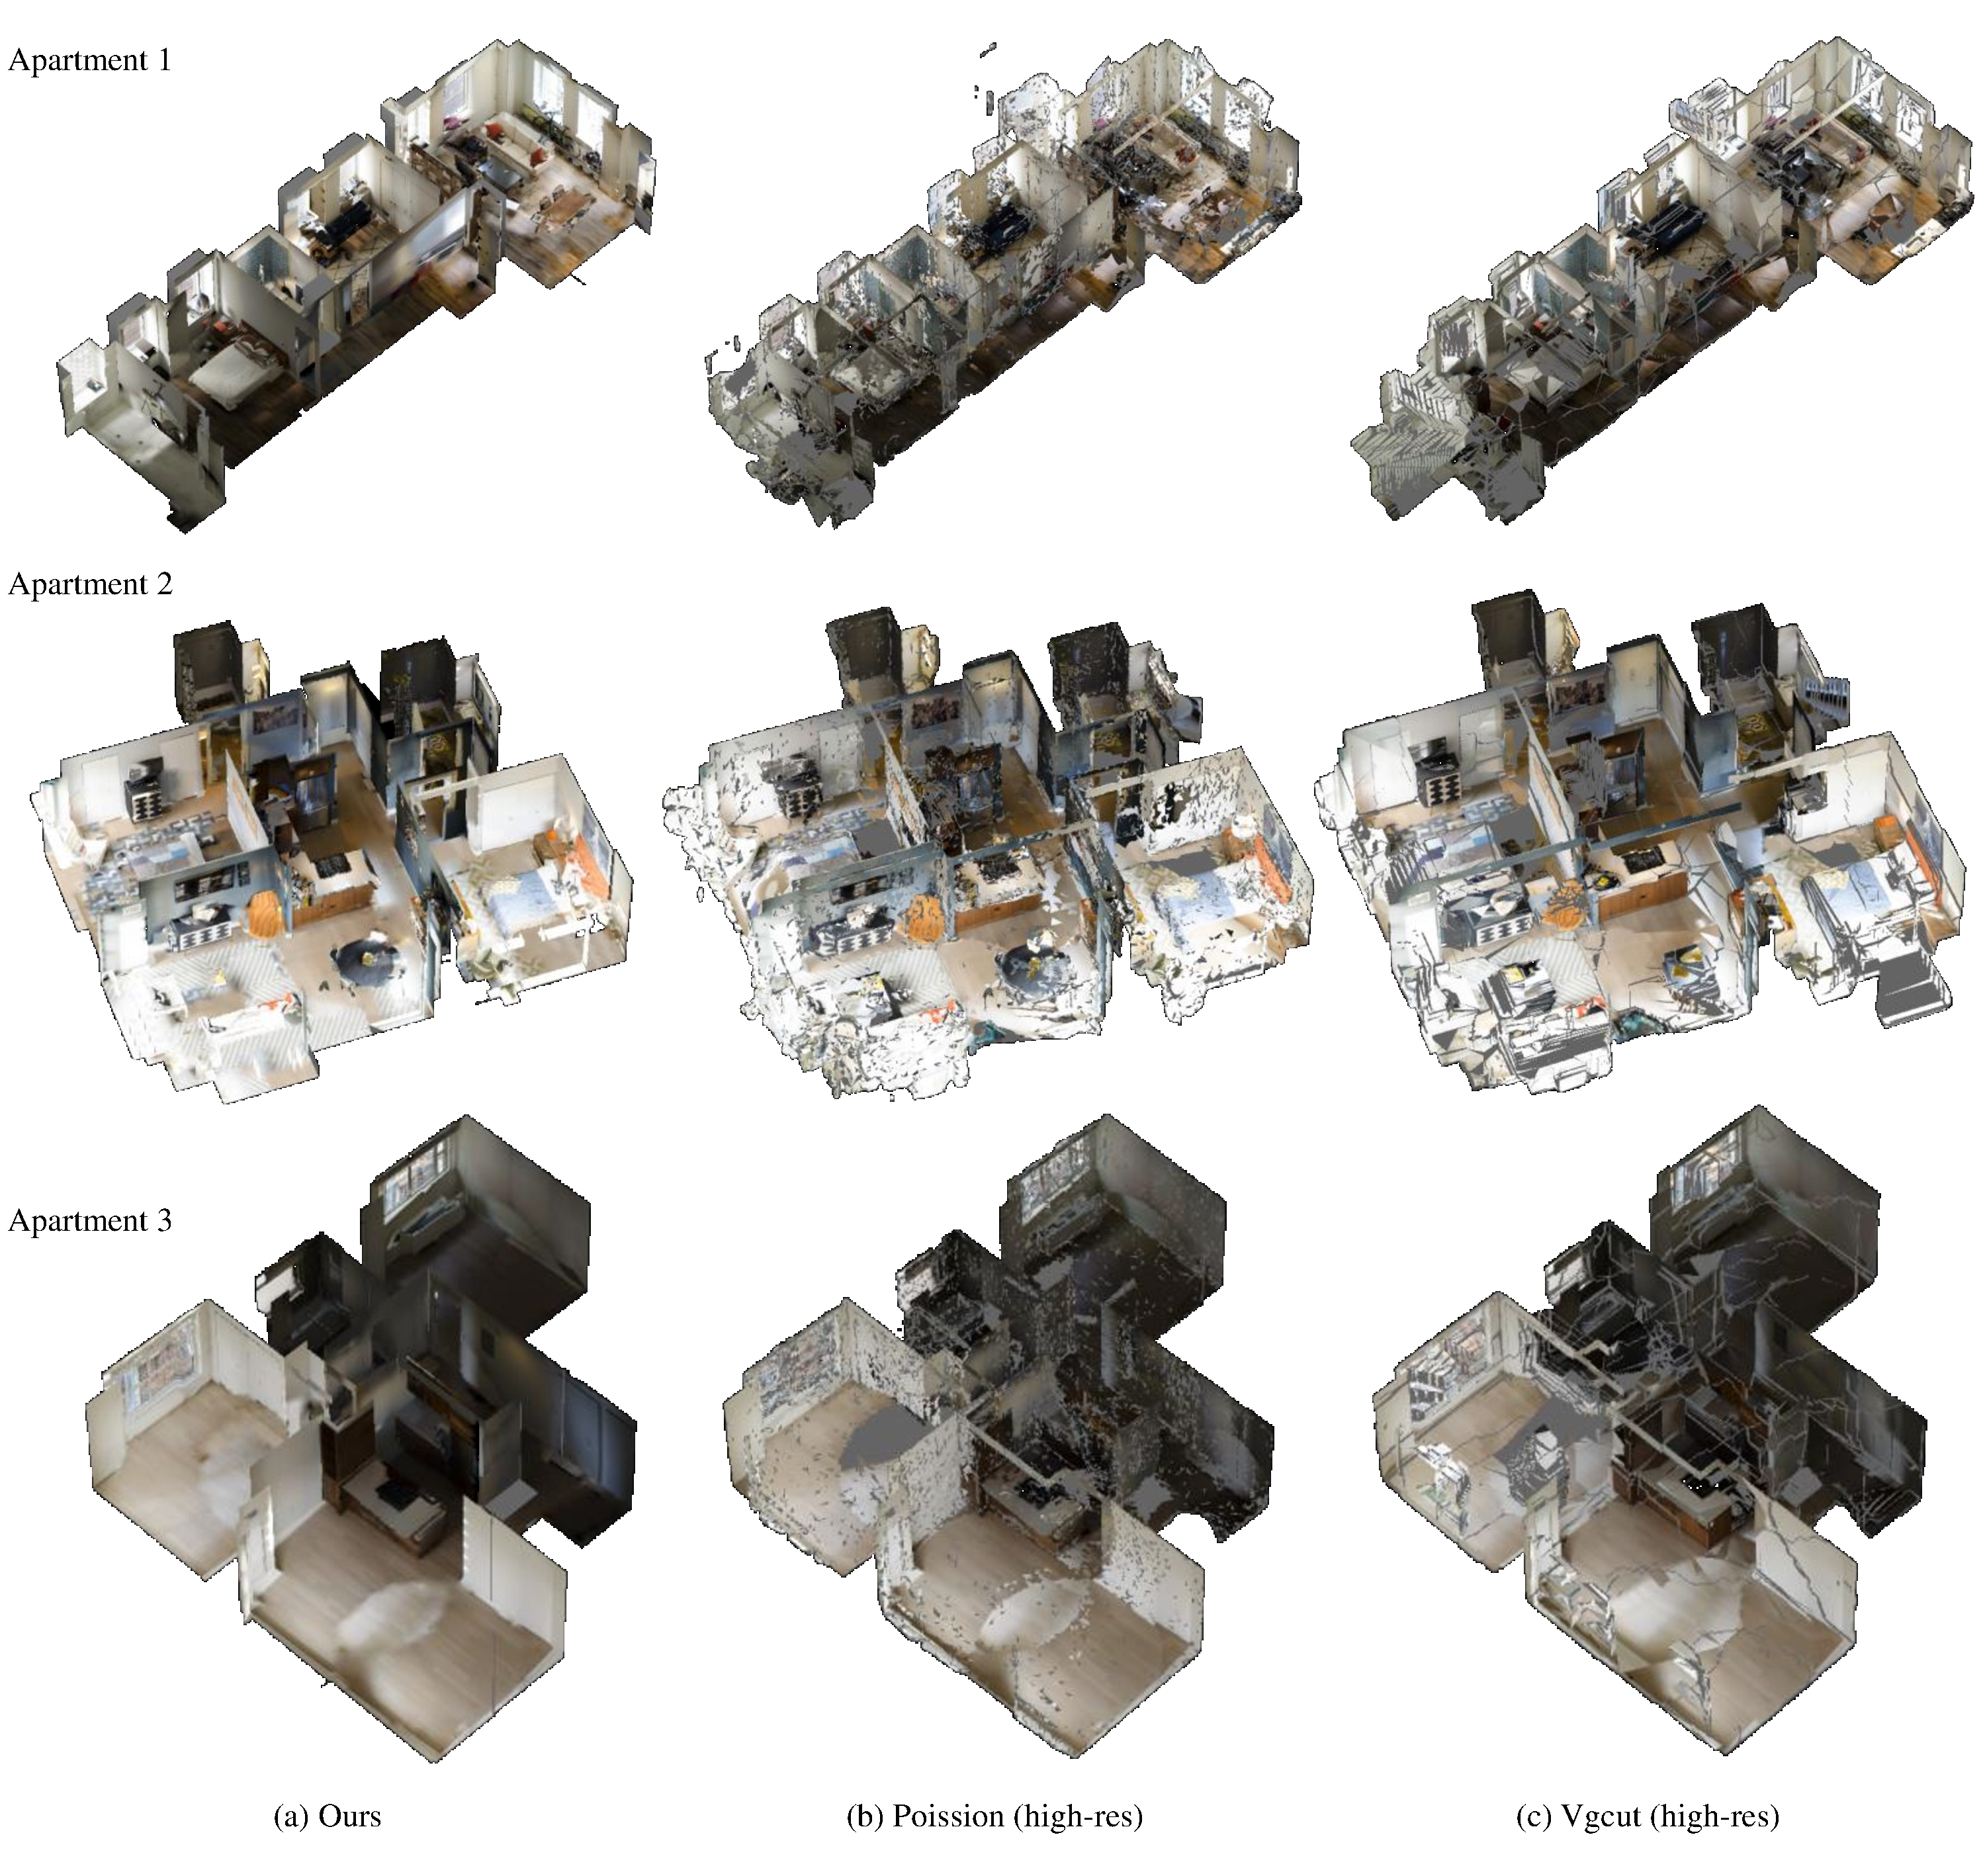
\includegraphics[width=\textwidth]{../figures/comp_meshes3.pdf}
 \end{center}
 \caption{Our structured model representation enables one to effectively
 hide (or add transparency to) back-facing surfaces such as ceilings and
 walls, at the level of structural elements as opposed to at the level of
 triangles. Meshes from existing algorithms only allow back-face culling per
 triangle and cause severe rendering artifacts for the aerial indoor
 scene visualization. }  \label{fig:comp_mesh0}
\end{figure*}

\clearpage
\begin{figure*}
 \begin{center}
%  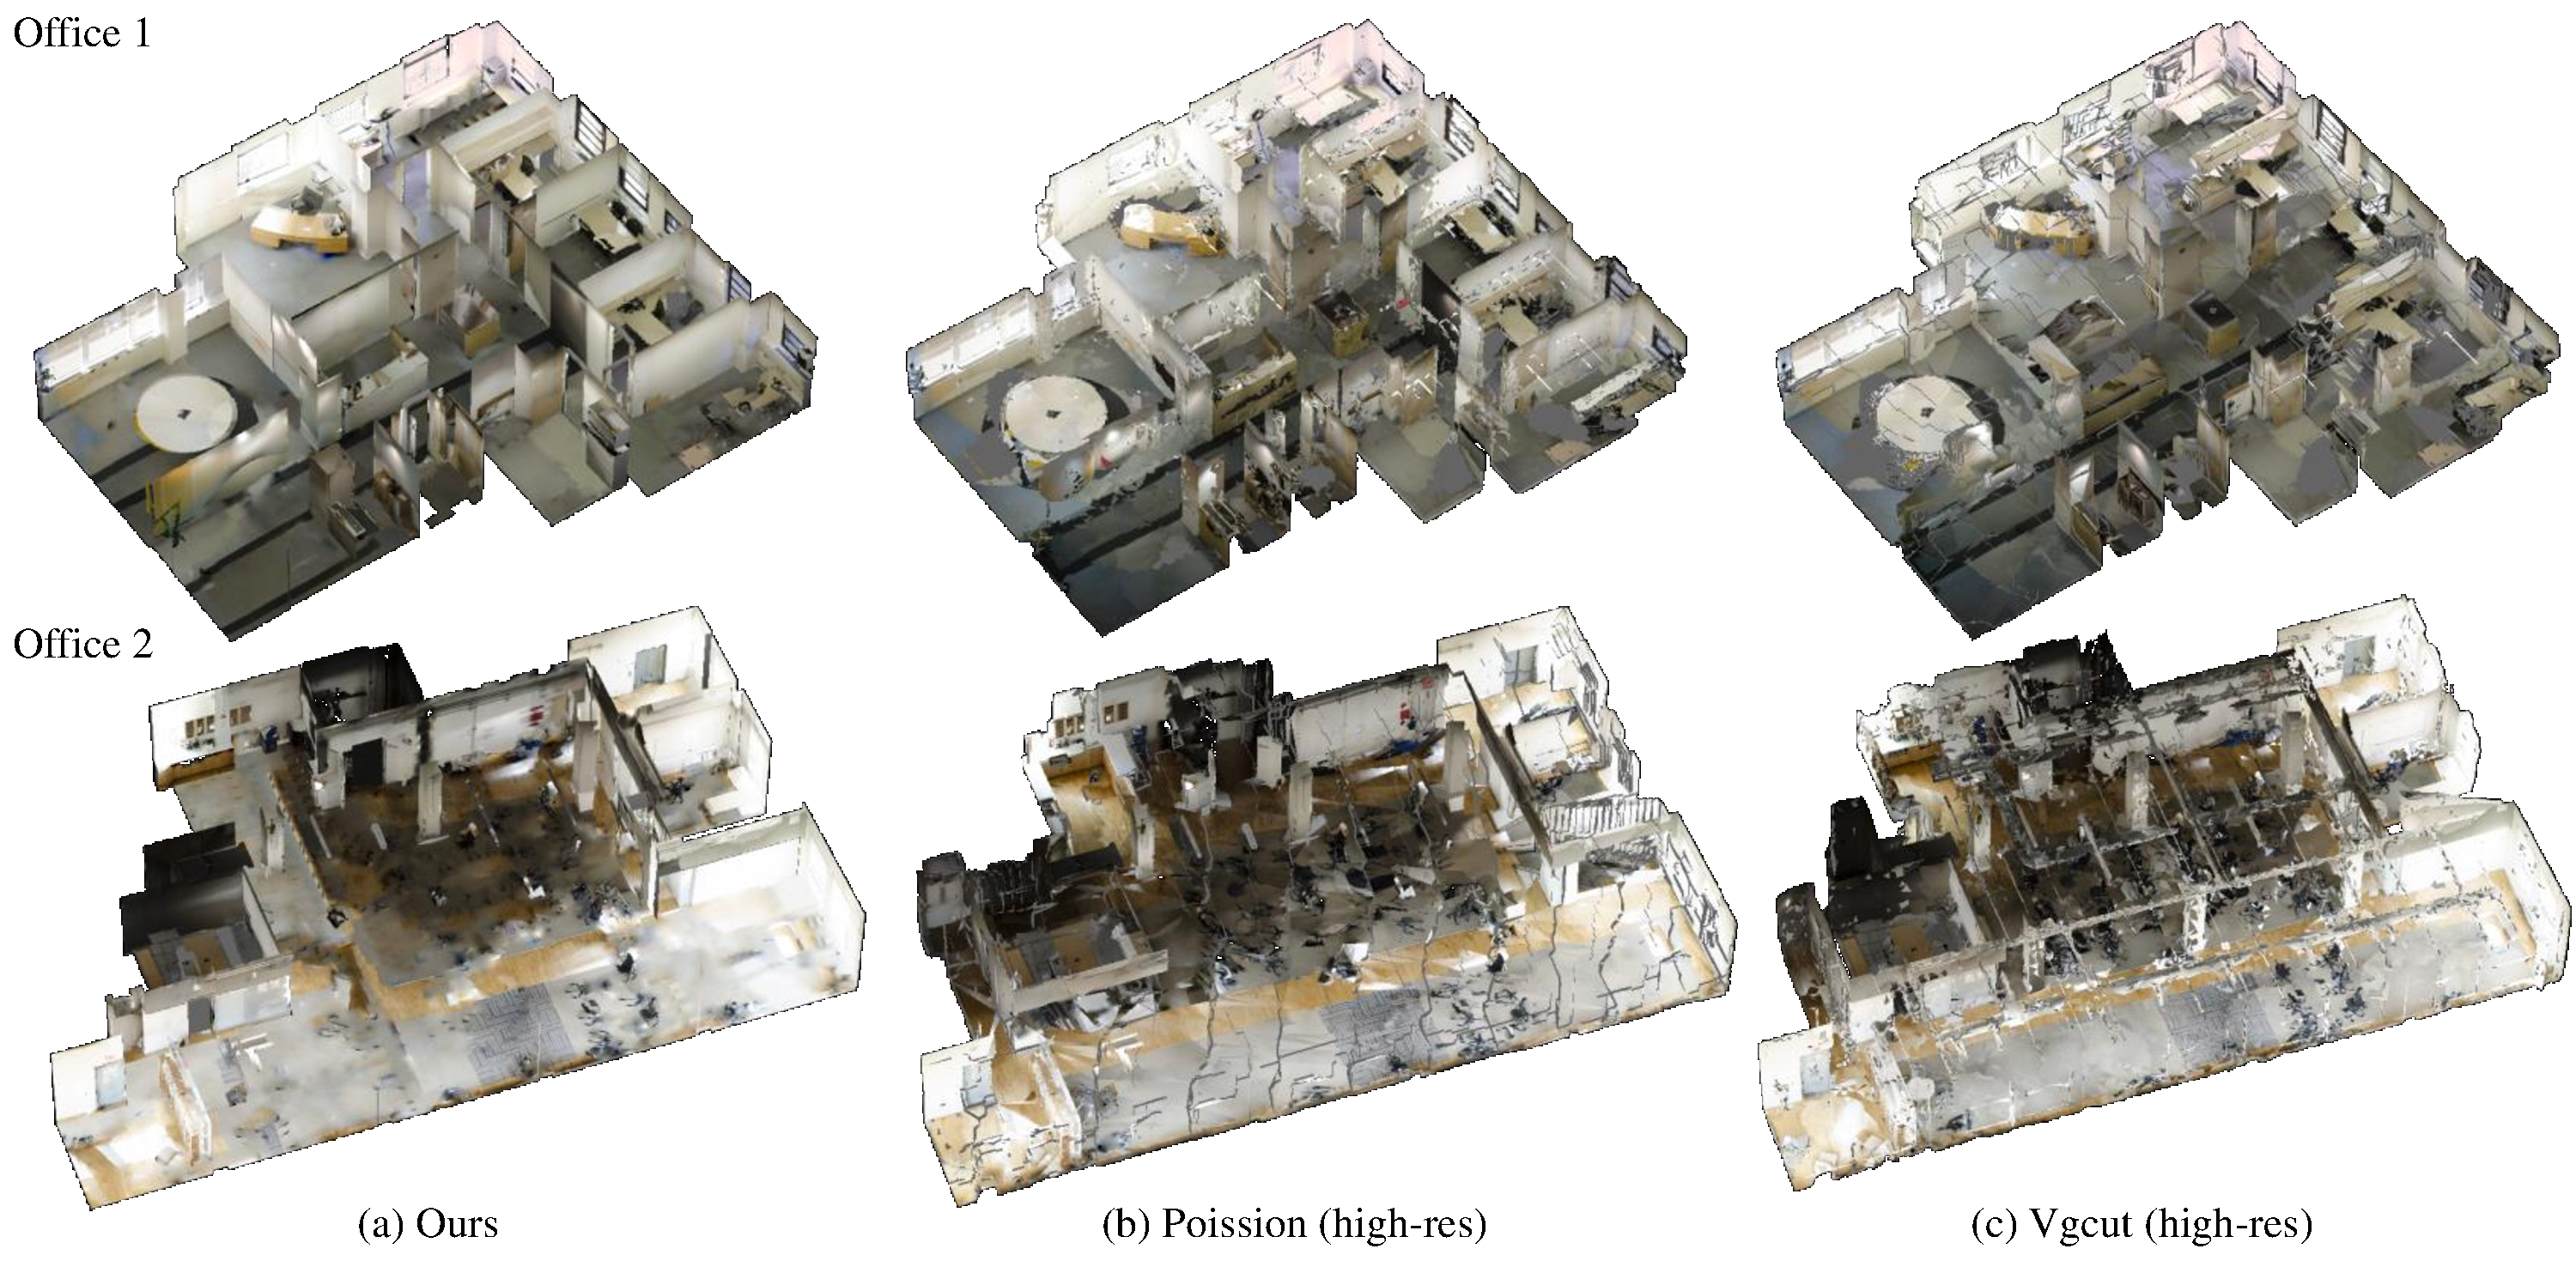
\includegraphics[width=\textwidth]{../figures/comp_meshes4.png}
    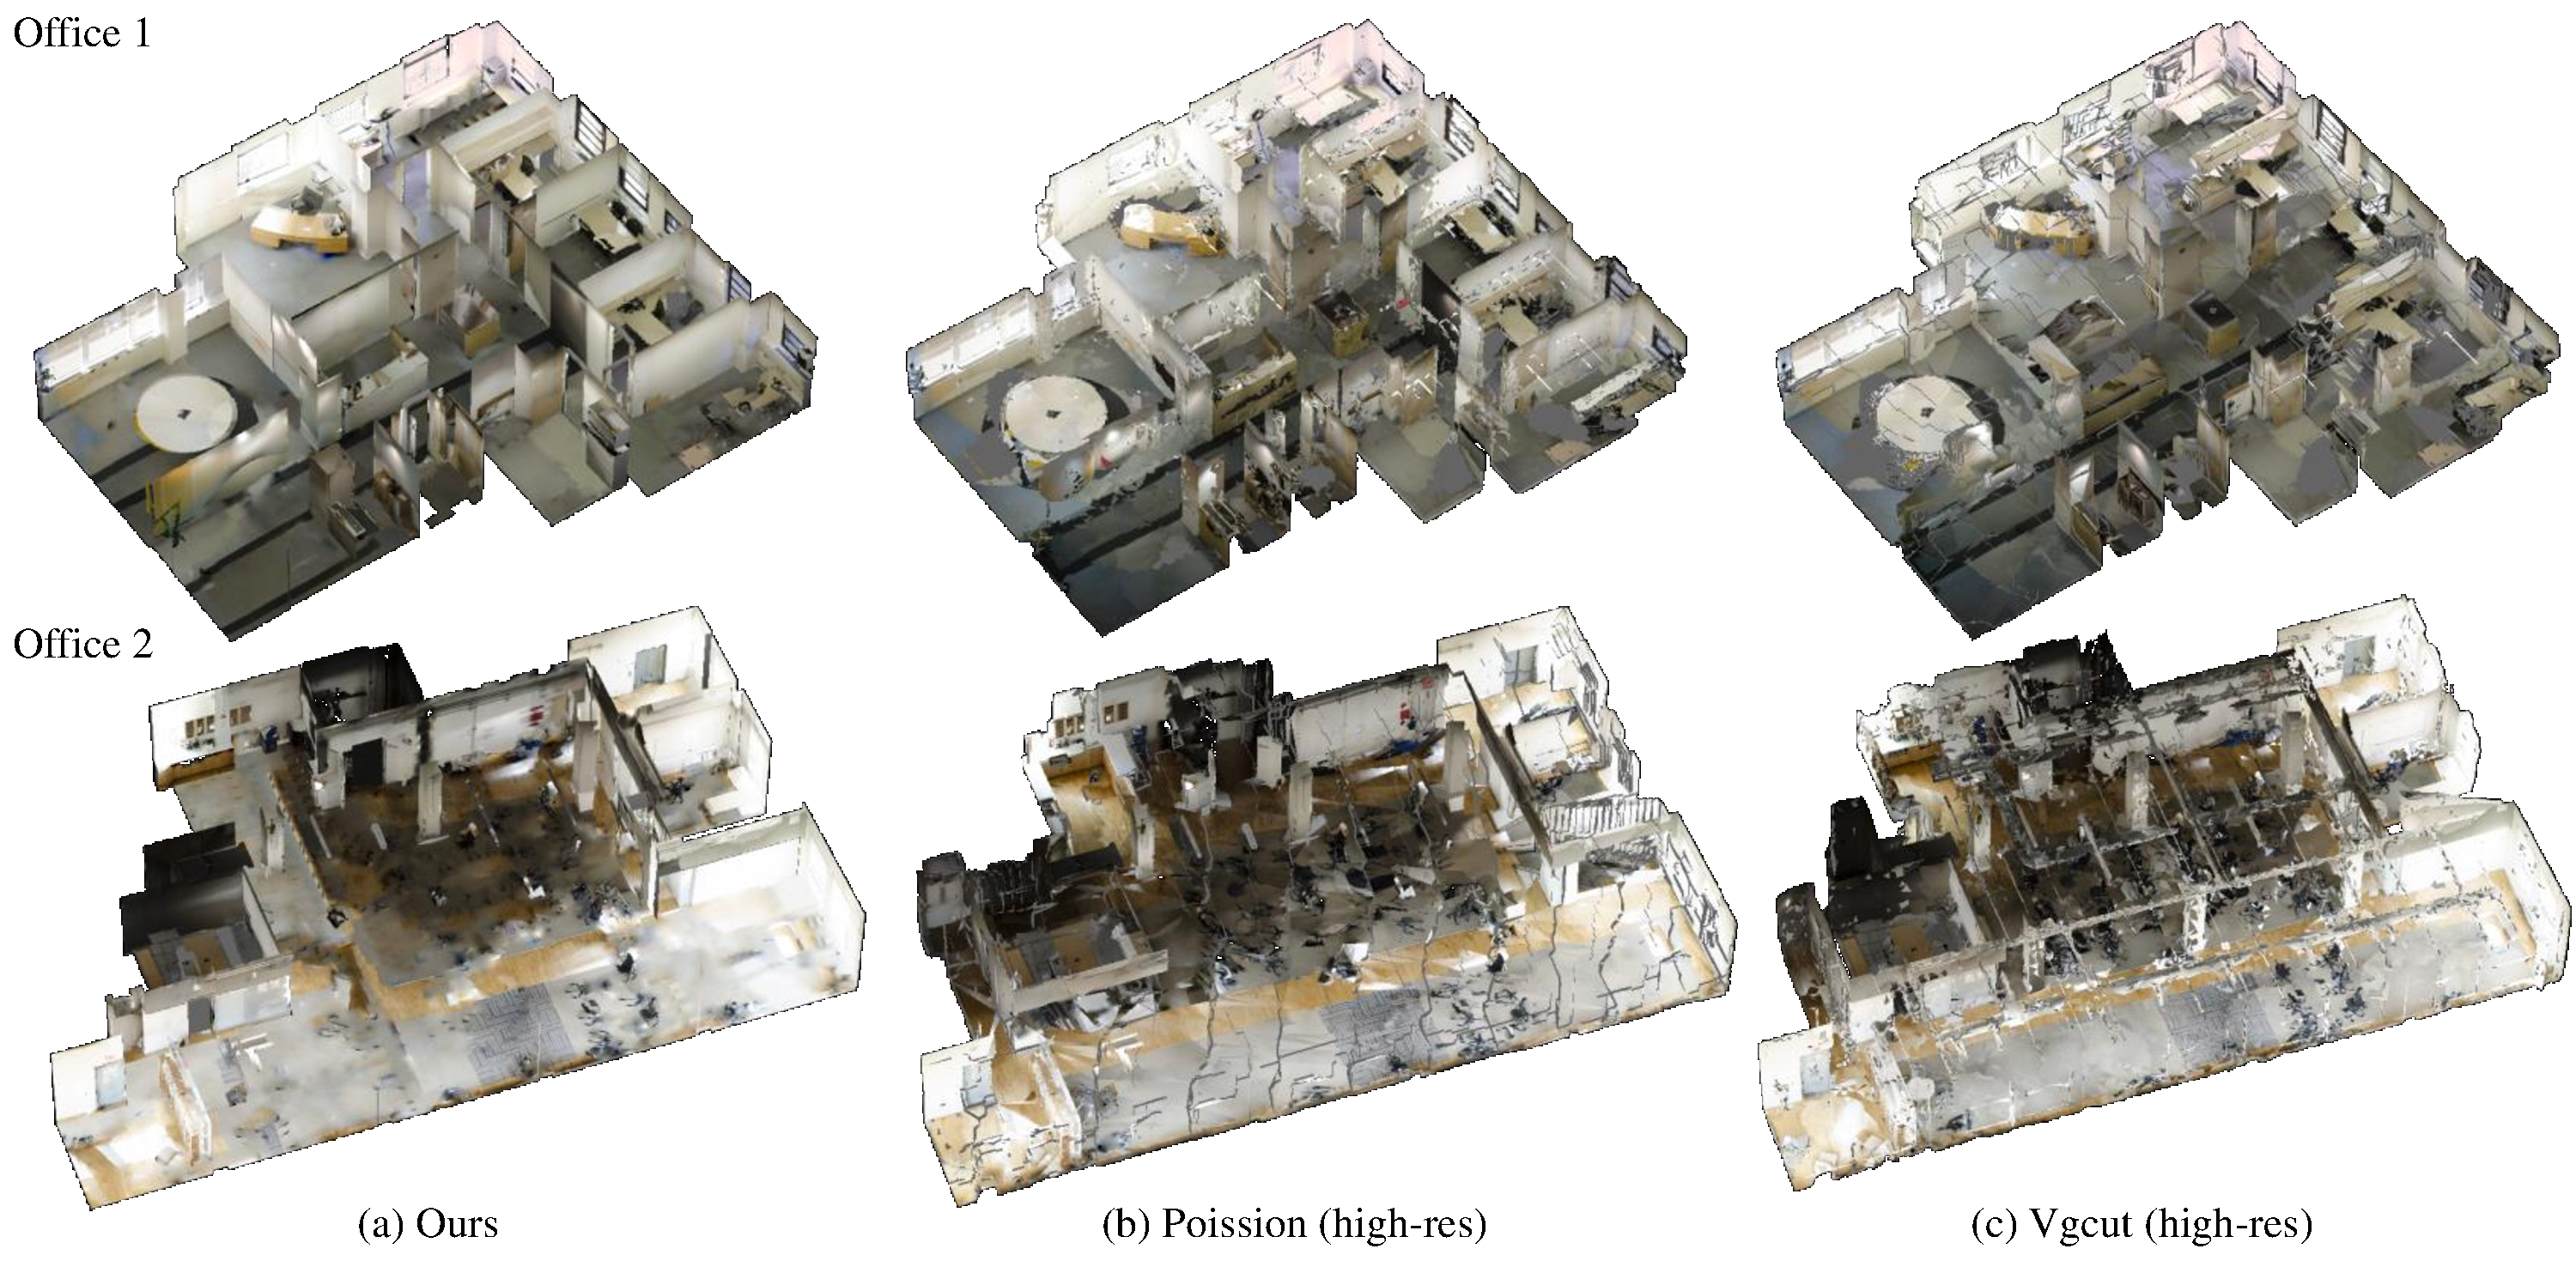
\includegraphics[width=\textwidth]{../figures/comp_meshes4.pdf}
 \end{center}
 \caption{Continued.}  \label{fig:comp_mesh1}
\end{figure*}


\clearpage
\begin{figure*}
 \begin{center}
  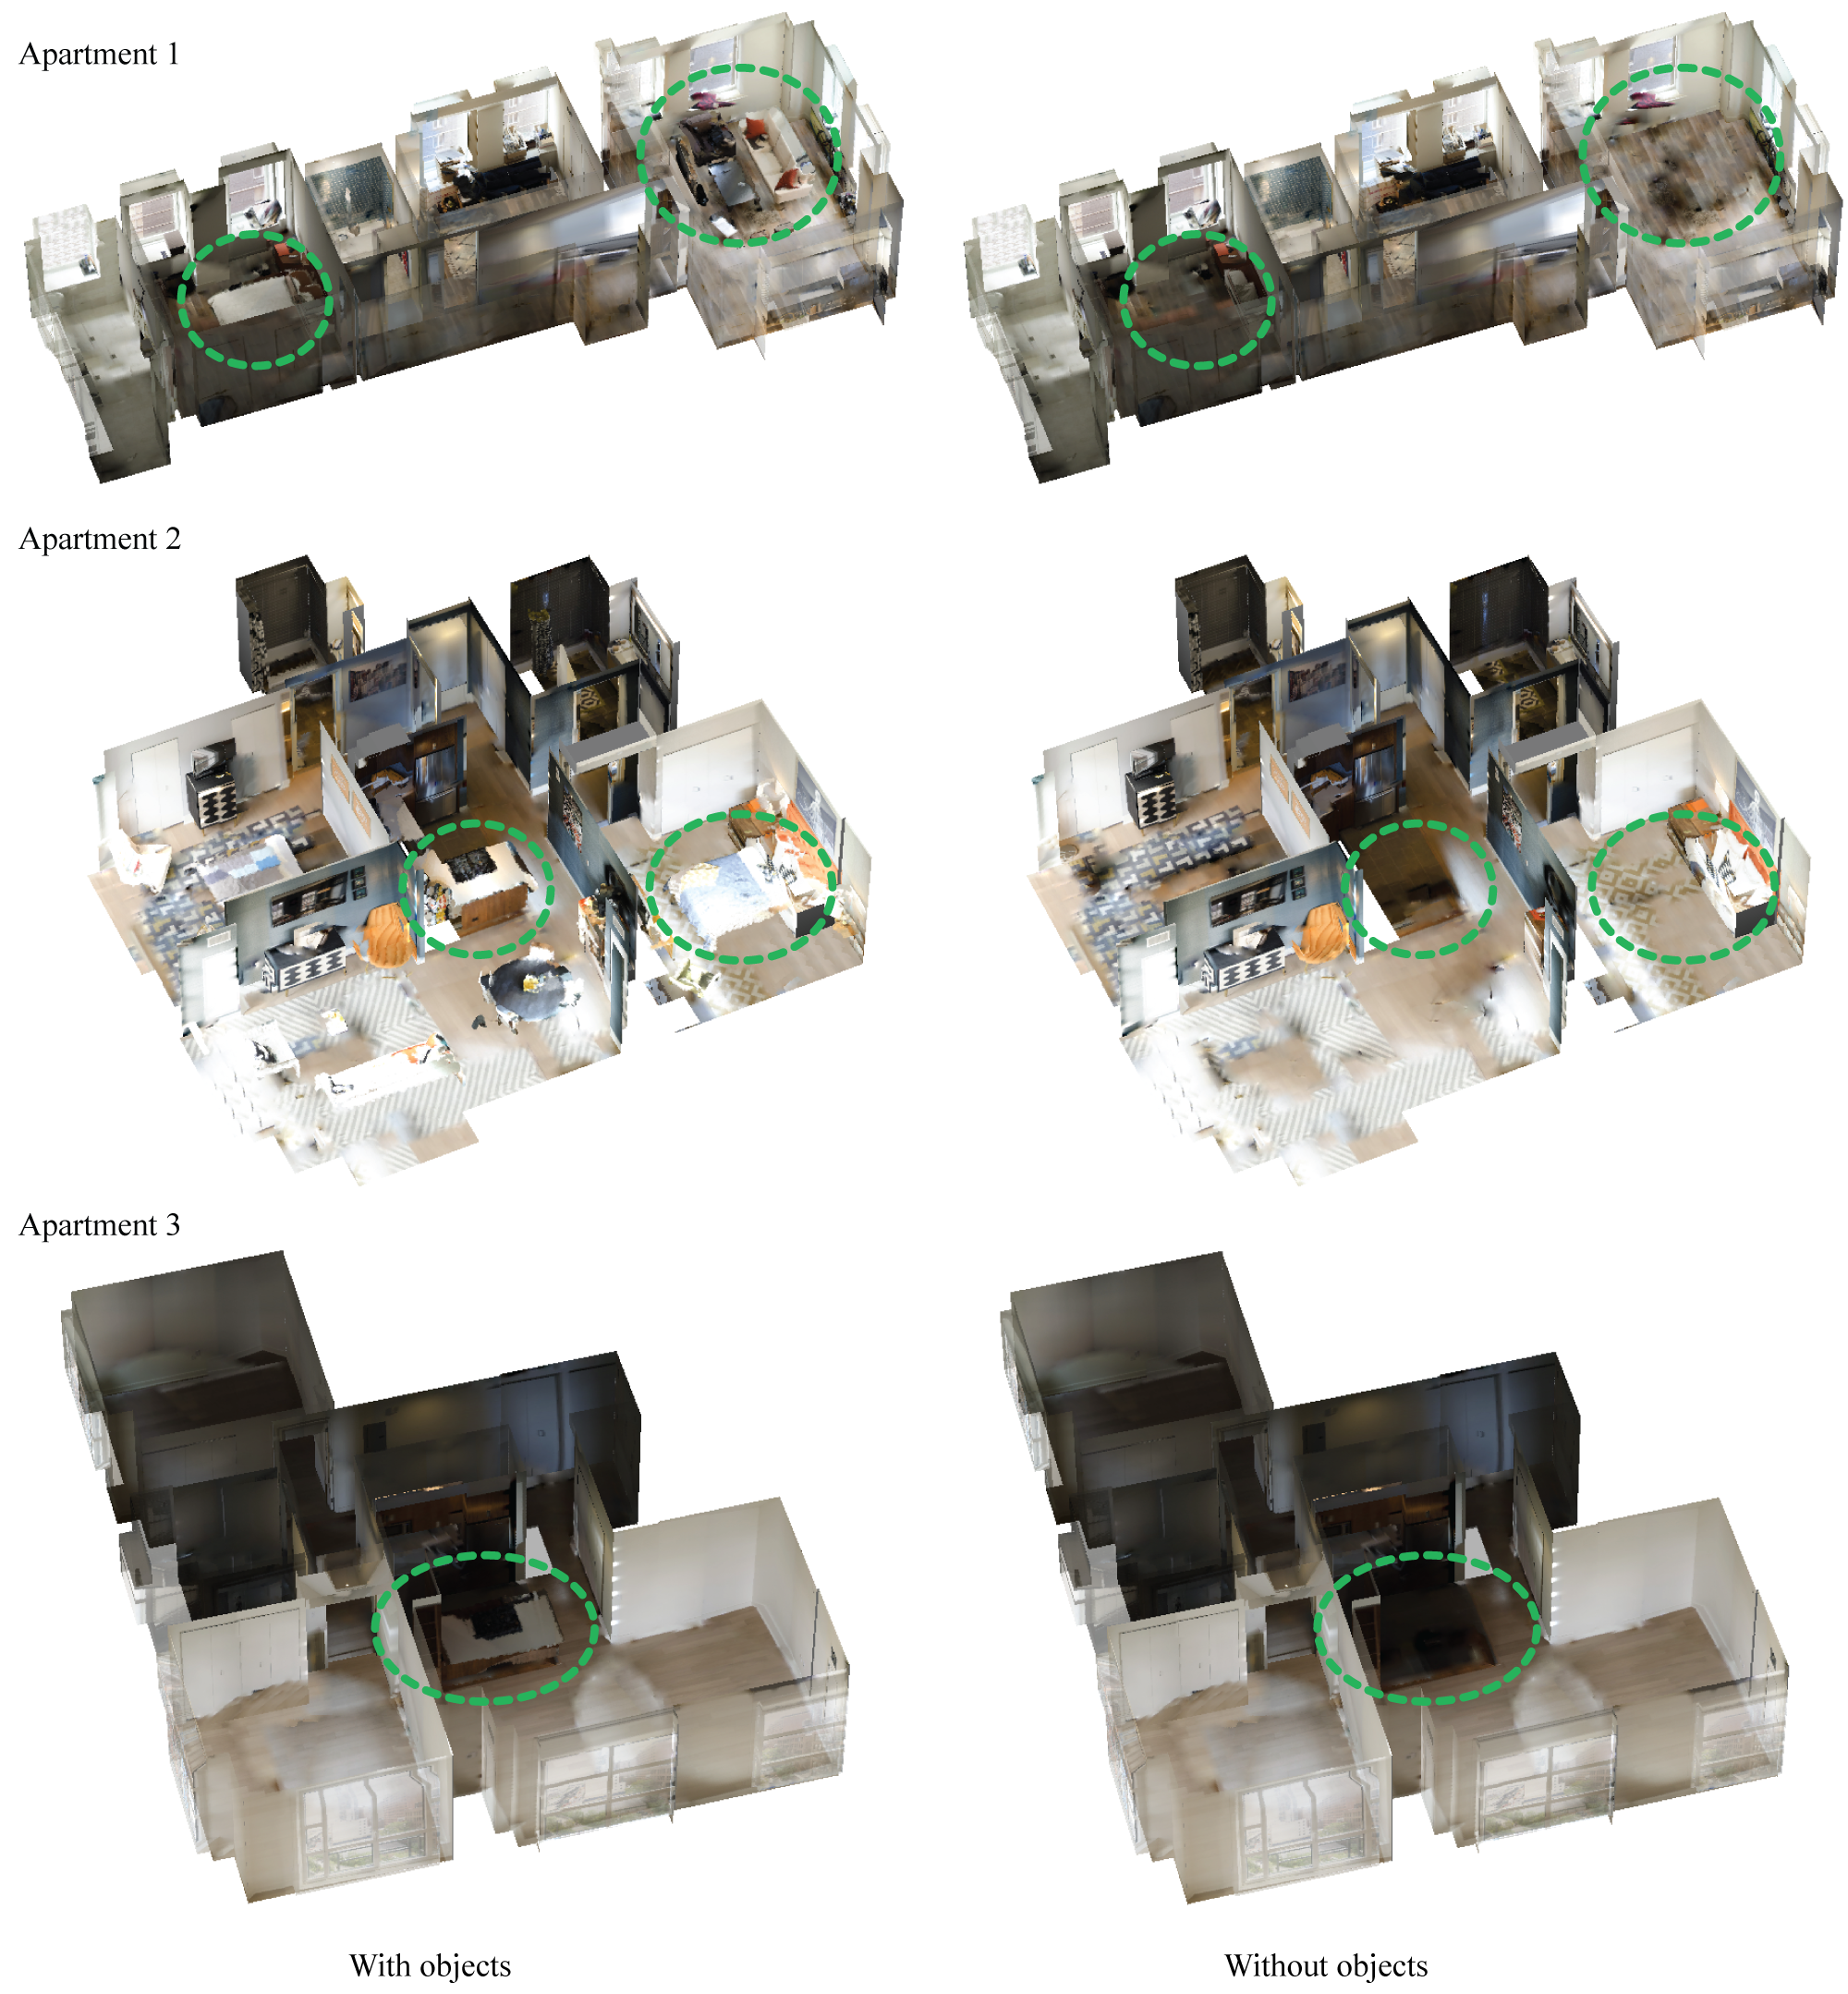
\includegraphics[width=\textwidth]{../figures/show_texture.png}
%    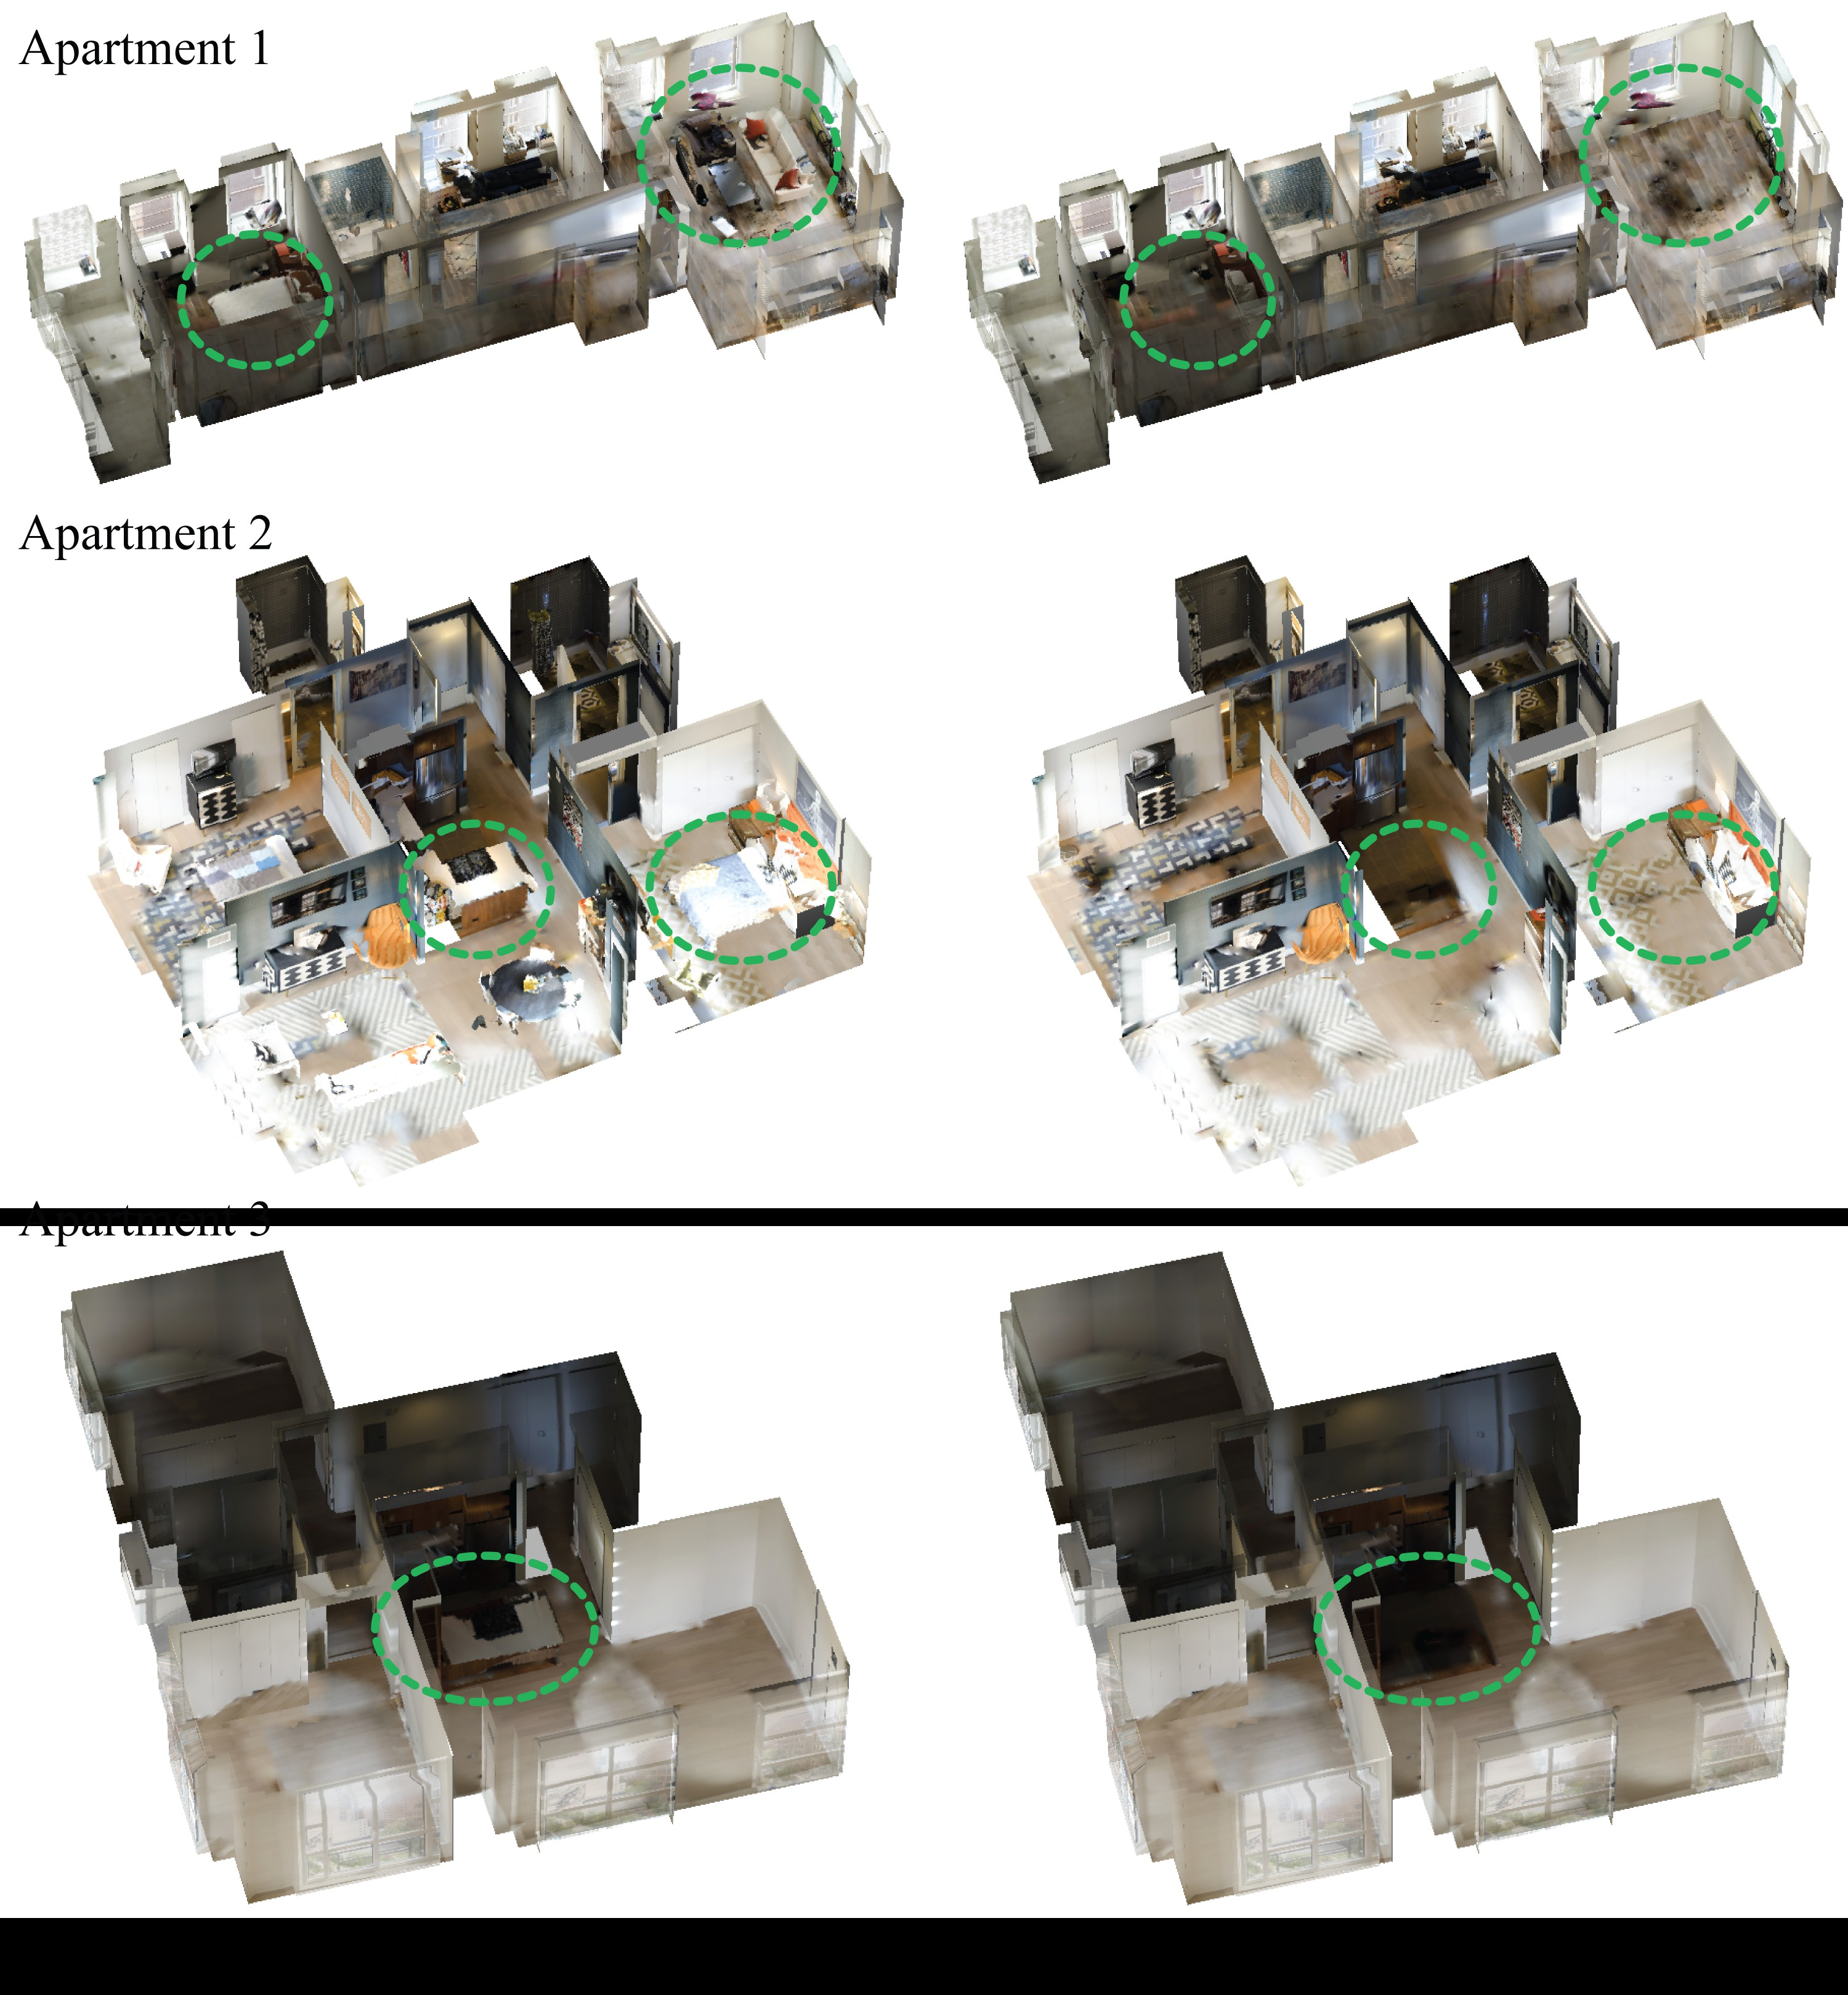
\includegraphics[width=\textwidth]{../figures/show_texture.jpg}
%      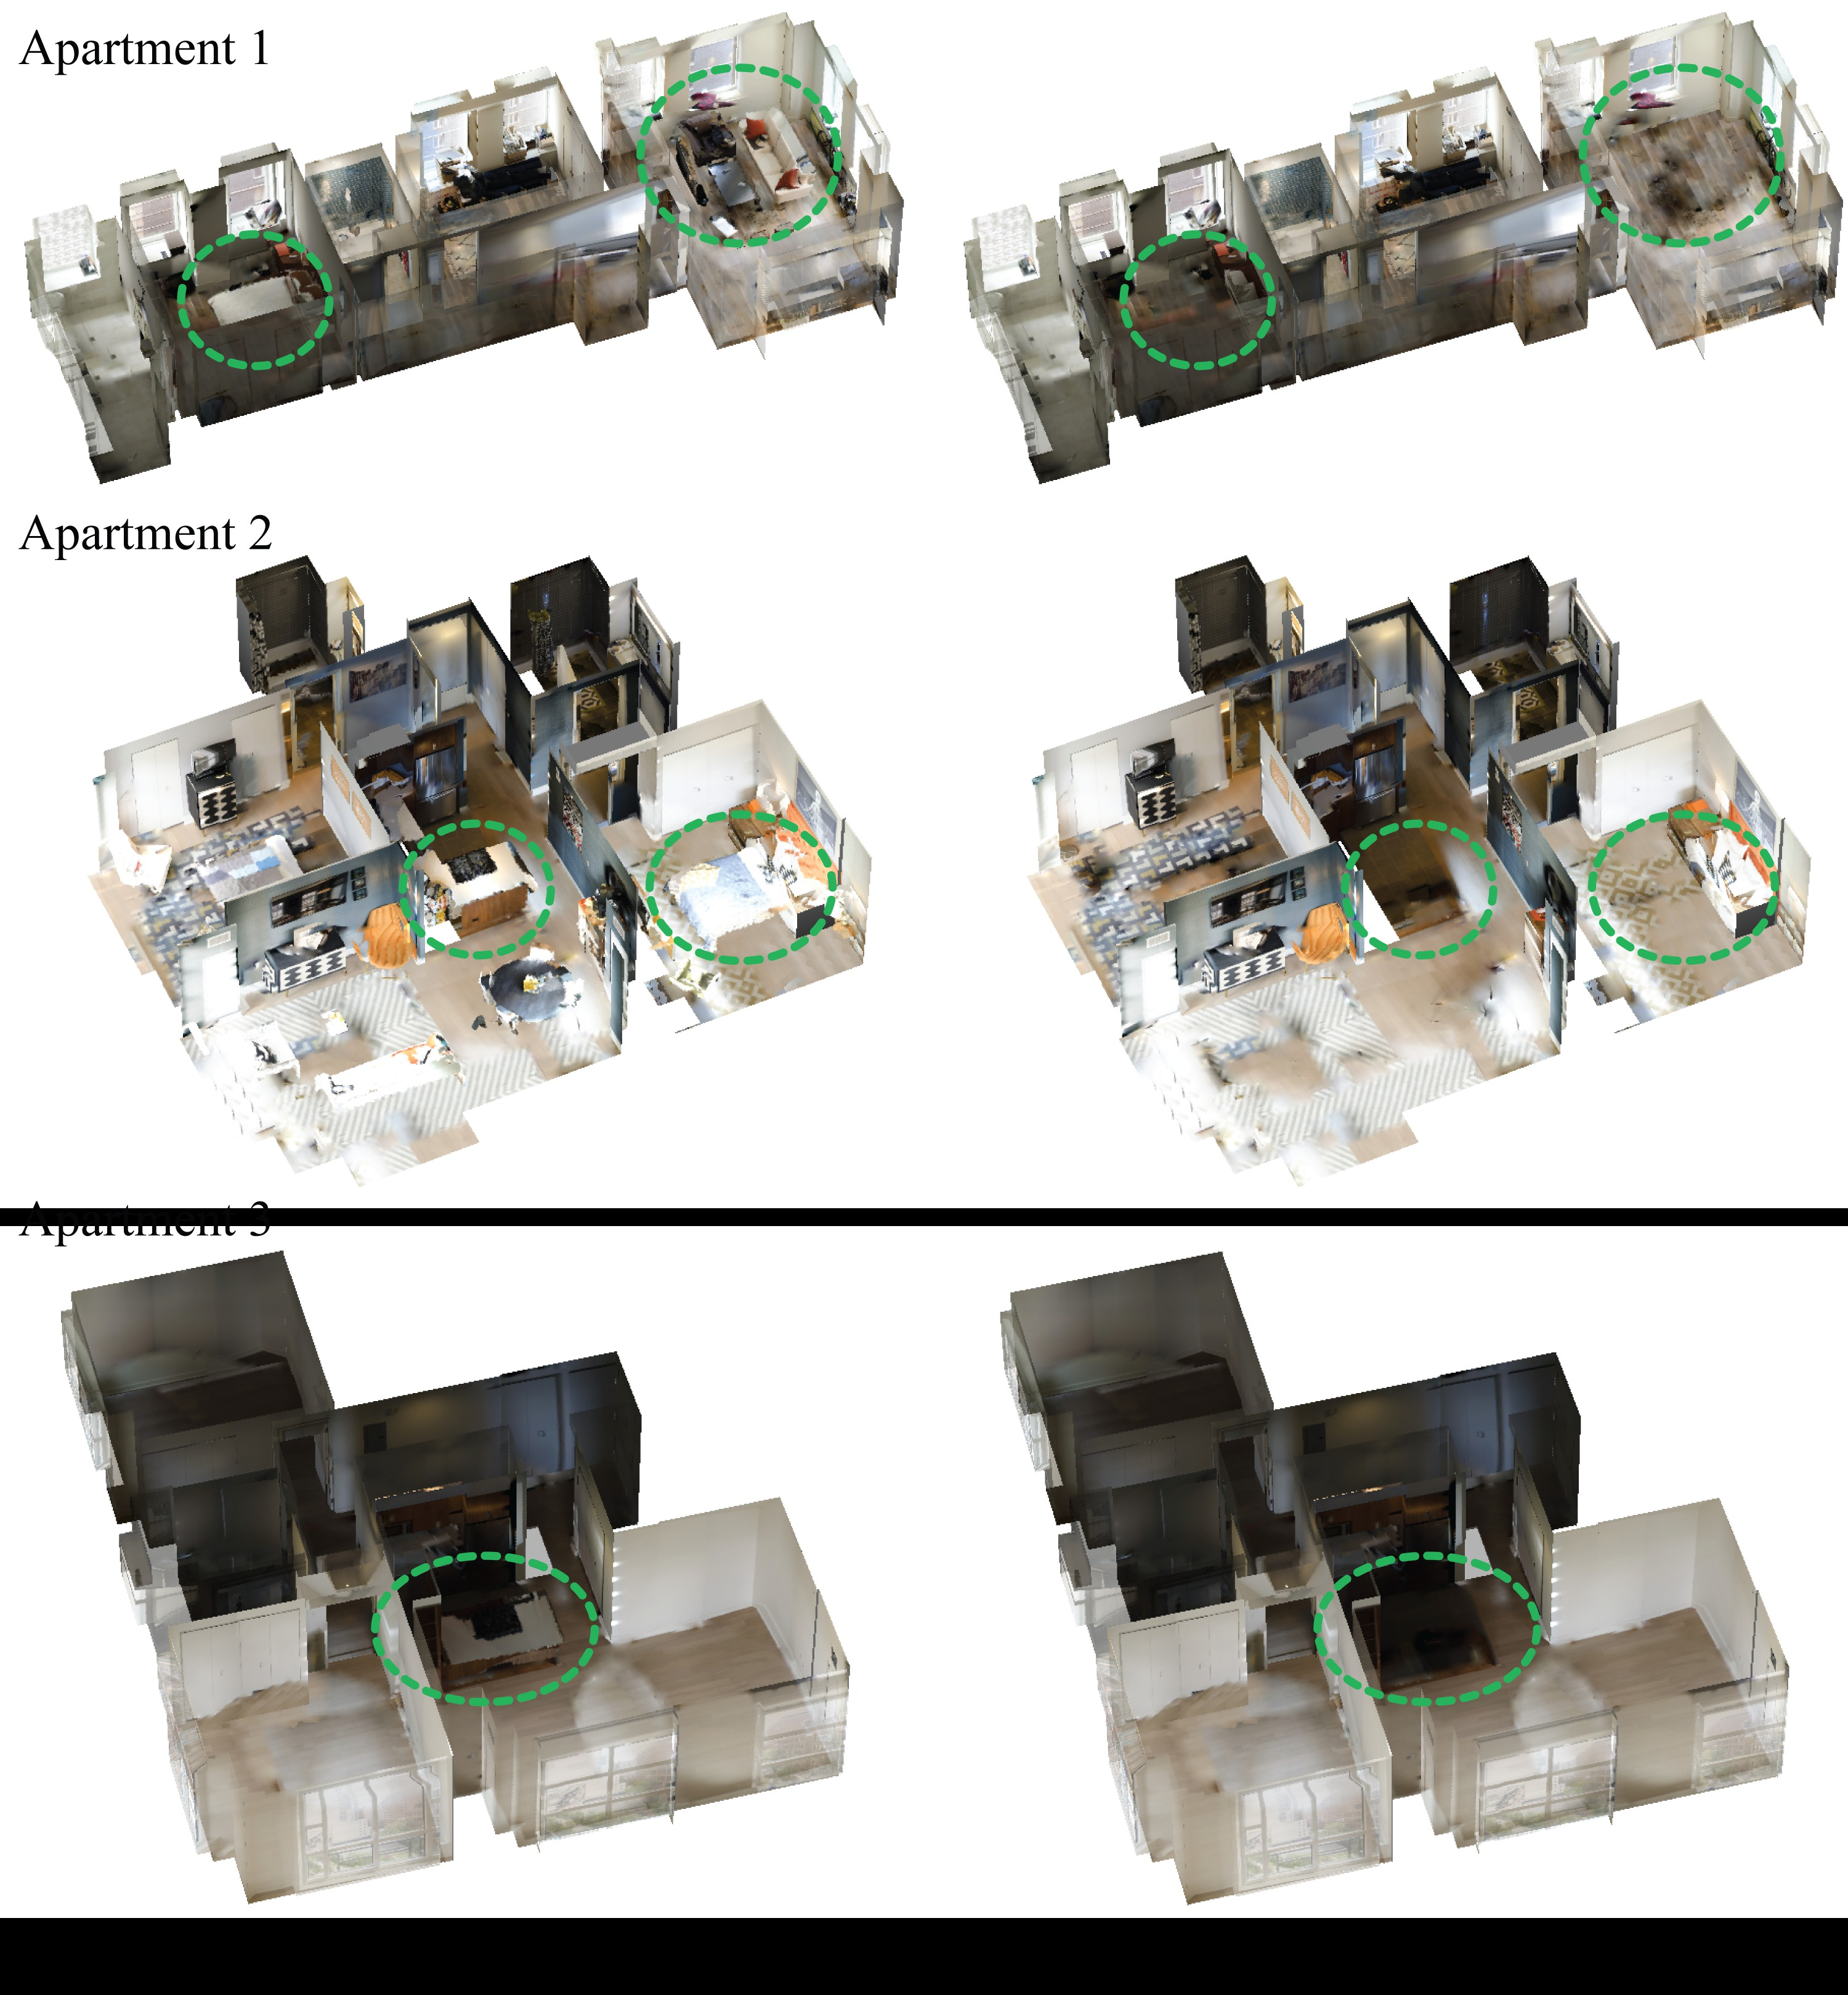
\includegraphics[width=\textwidth]{../figures/show_texture.pdf}
 \end{center}
 \caption{The left and right shows our model with and without objects
 rendered.  Textures on the mesh models are computed for each piecewise
 planar surface by a combination of texture synthesis and inpainting
 techniques. Our structured representation essentially allows us to
 compute the texture for each structural element such as walls and
 floors, can effectively fill texture holes even behind objects.}
 \label{fig:texture0}
\end{figure*}

\clearpage
\begin{figure*}
 \begin{center}
  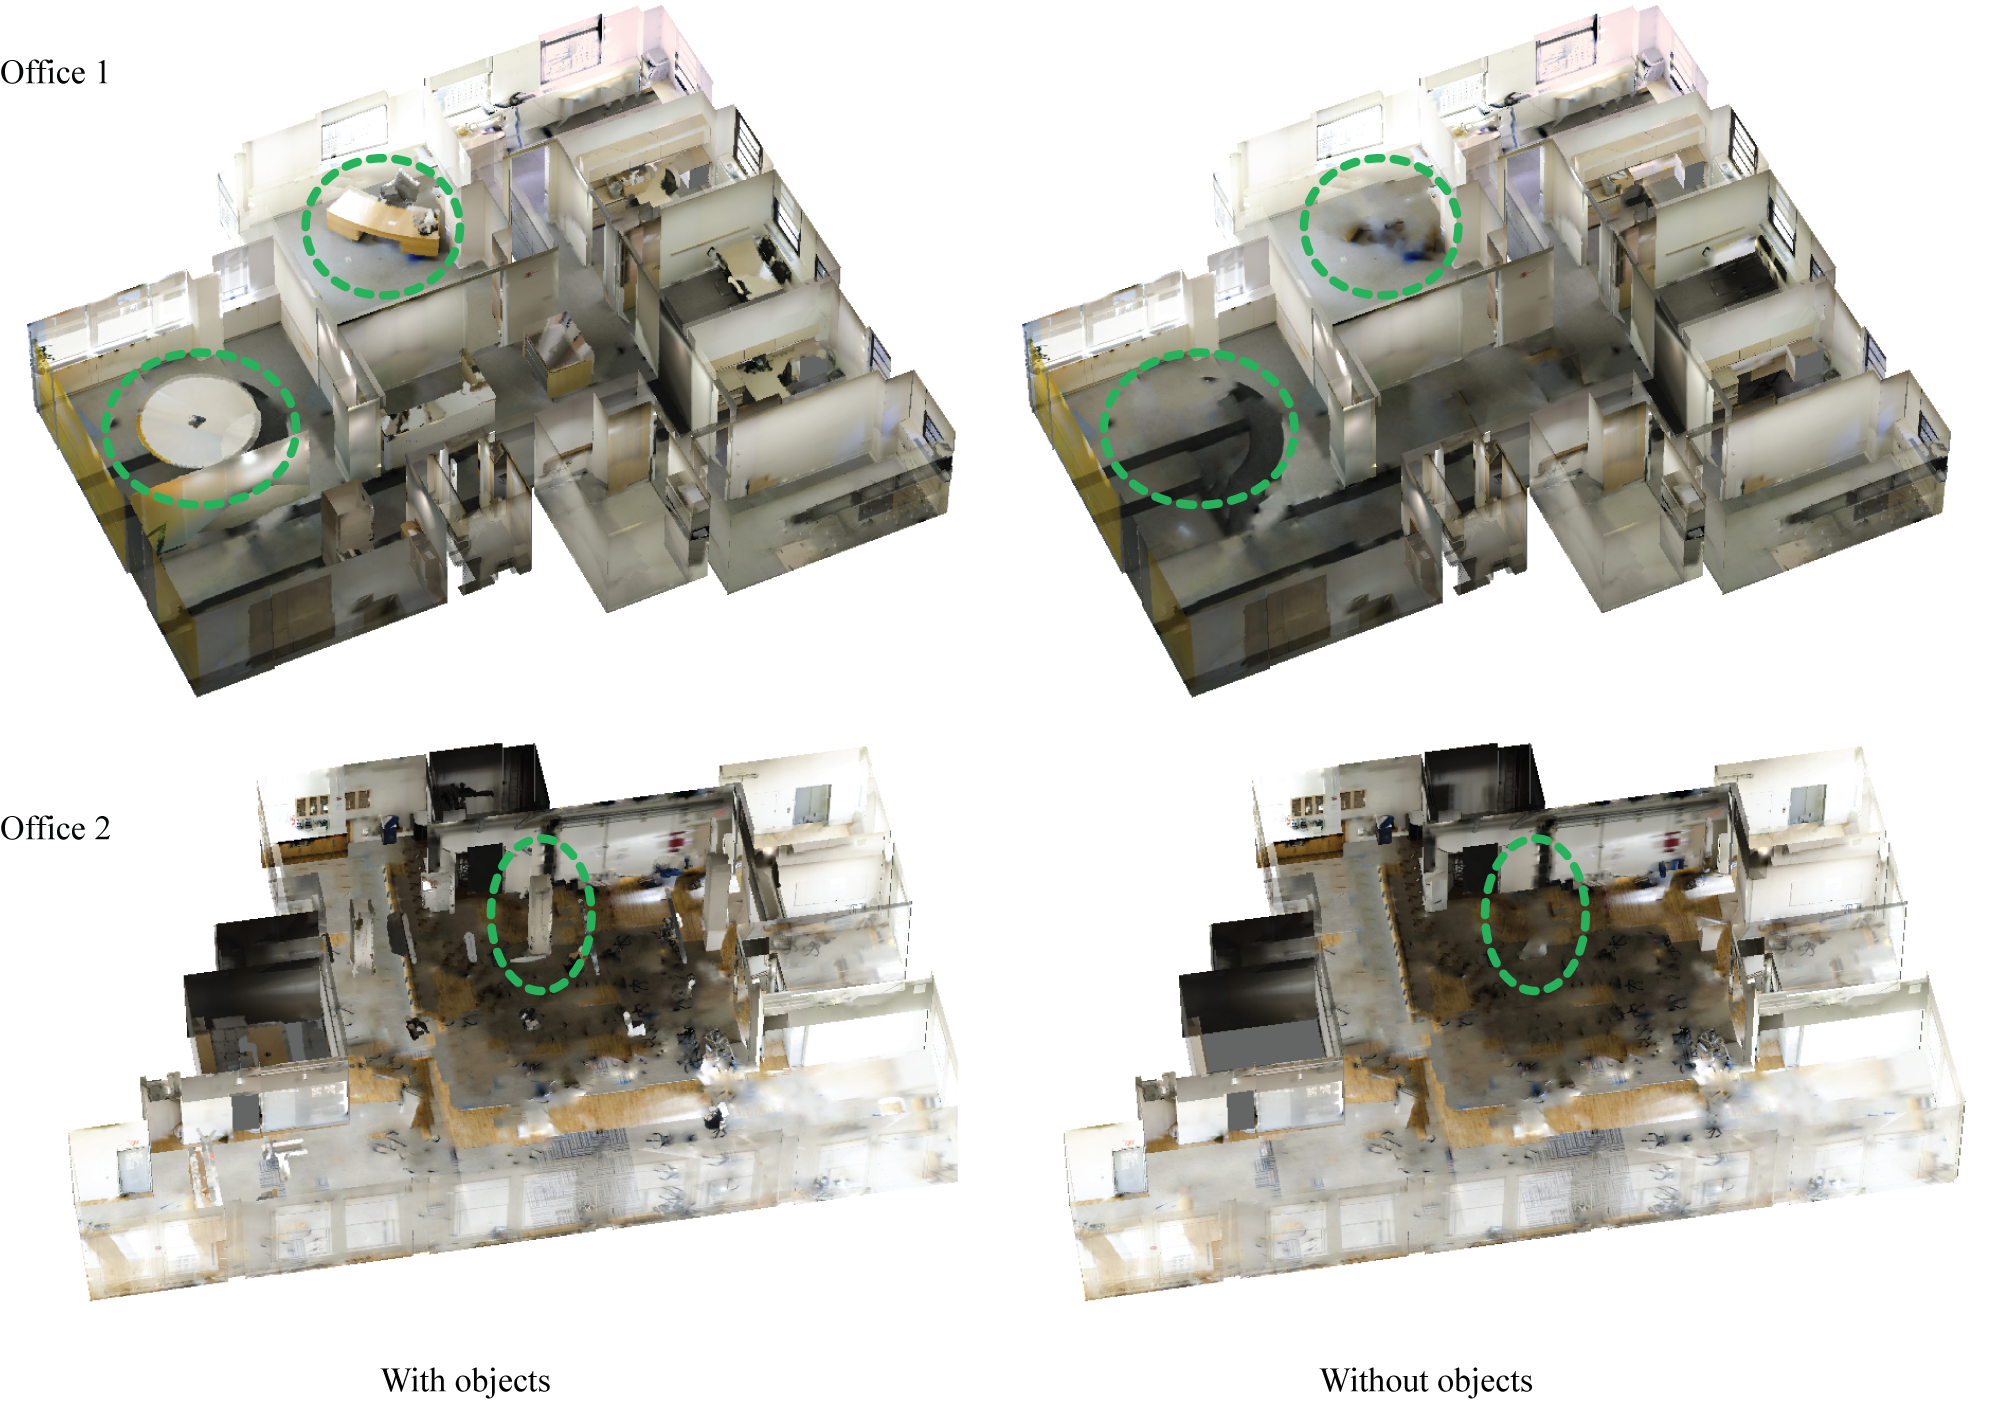
\includegraphics[width=\textwidth]{../figures/show_texture2.png}
%    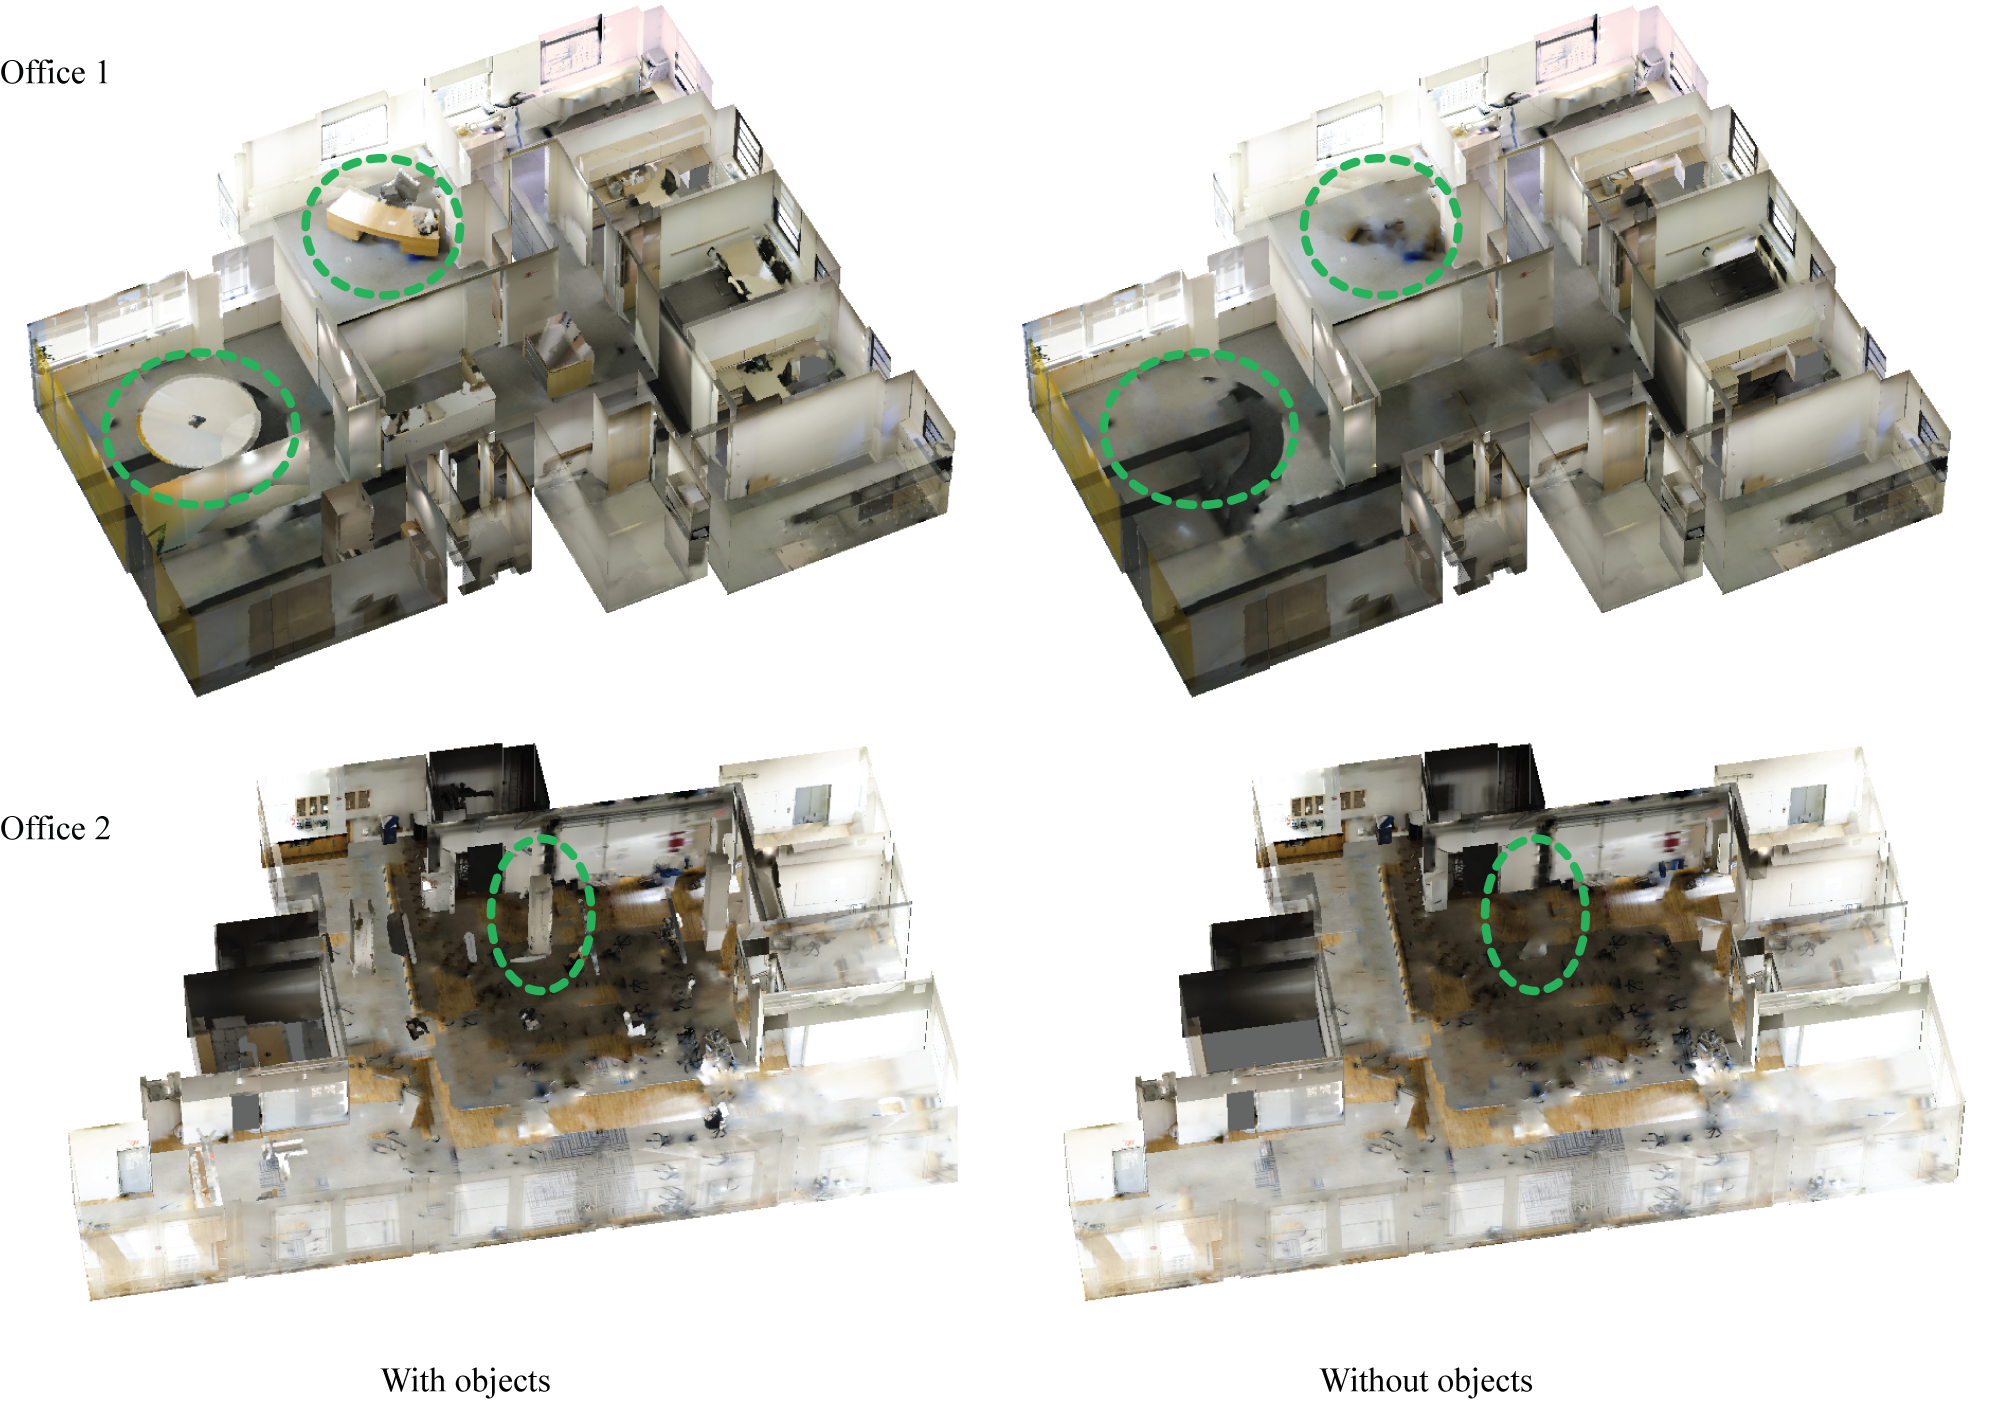
\includegraphics[width=\textwidth]{../figures/show_texture2.pdf}
 \end{center}
 \caption{Continued.}  \label{fig:texture1}
\end{figure*}


\clearpage
\begin{figure*}[!t]
  \centering
%  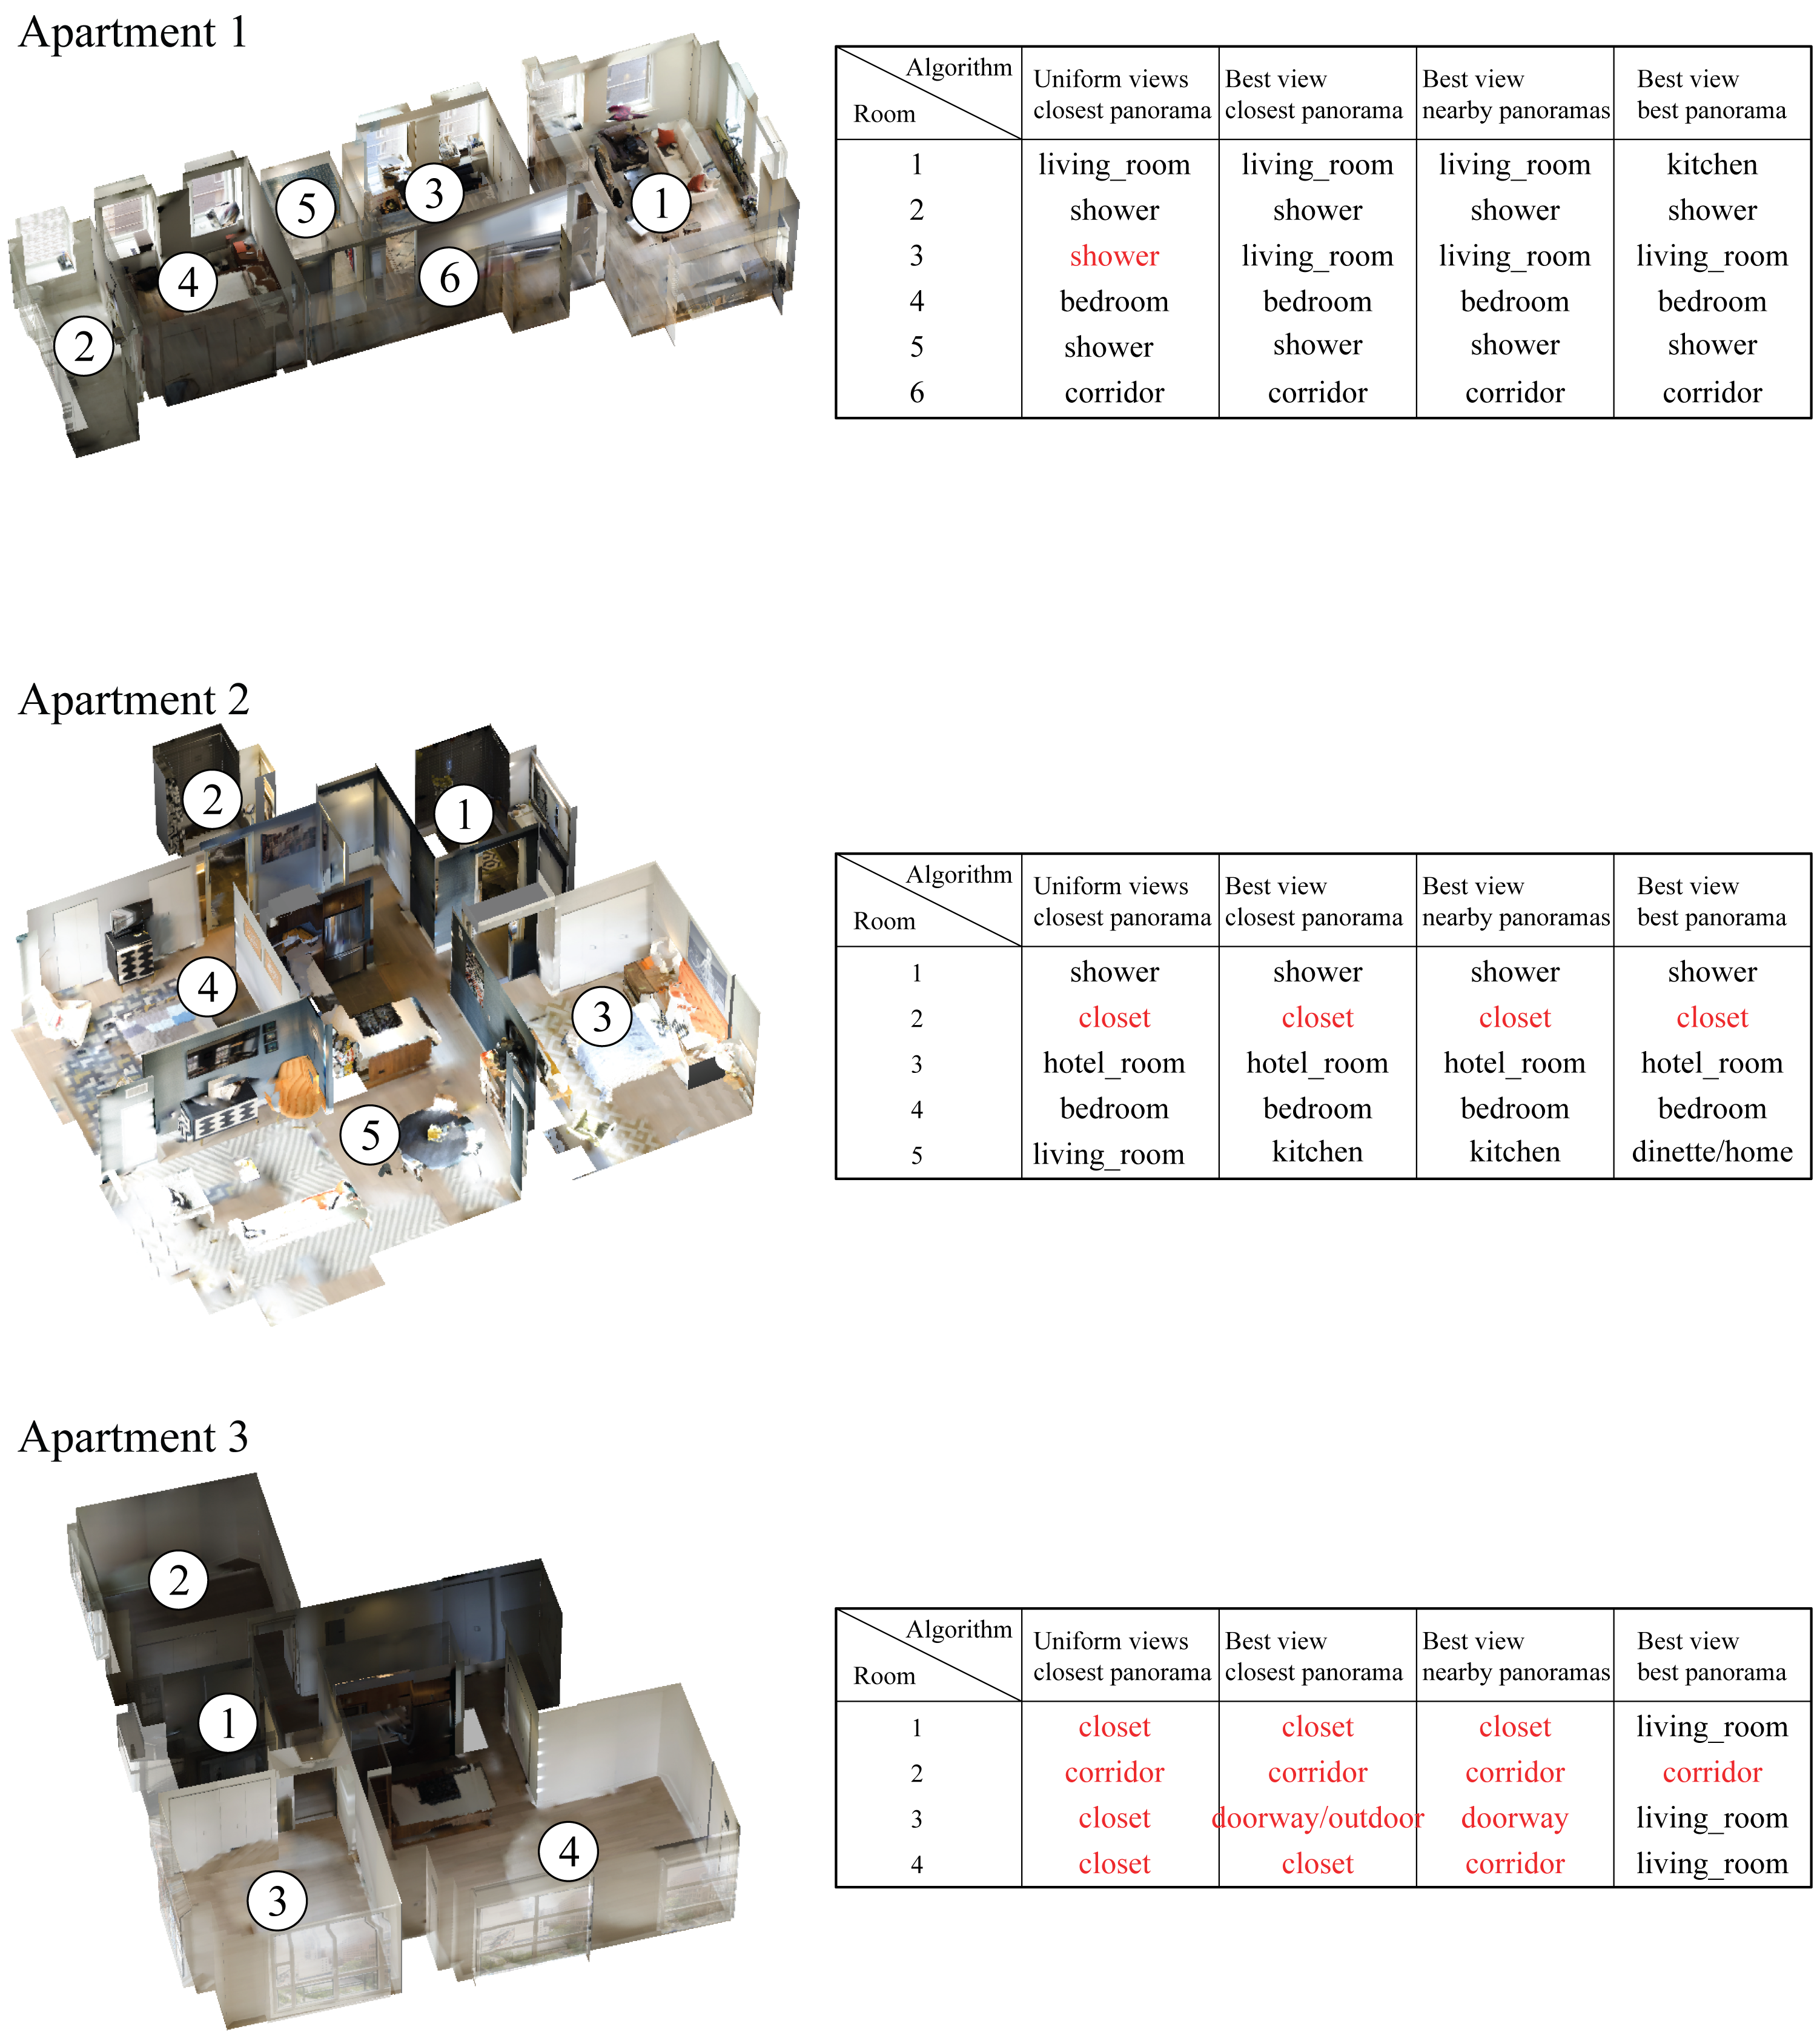
\includegraphics[width=\textwidth]{../figures/room_recognition_stats0.png}
   \includegraphics[width=\textwidth]{../figures/room_recognition_stats00.pdf}
  \caption{Room annotations are obtained by using the state-of-the-art
 scene recognition system~\cite{mit_scene_demo_paper}. We experimented four
 different algorithms in choosing images to represent each room,
 yielding large performance variations. The annotation result for each
 room by each algorithm is shown in the table. We manually verified the
 results and highlight mistakes in red.}
 \label{fig:room_recog}
\end{figure*}

\clearpage
\begin{figure*}[!t]
  \centering
%  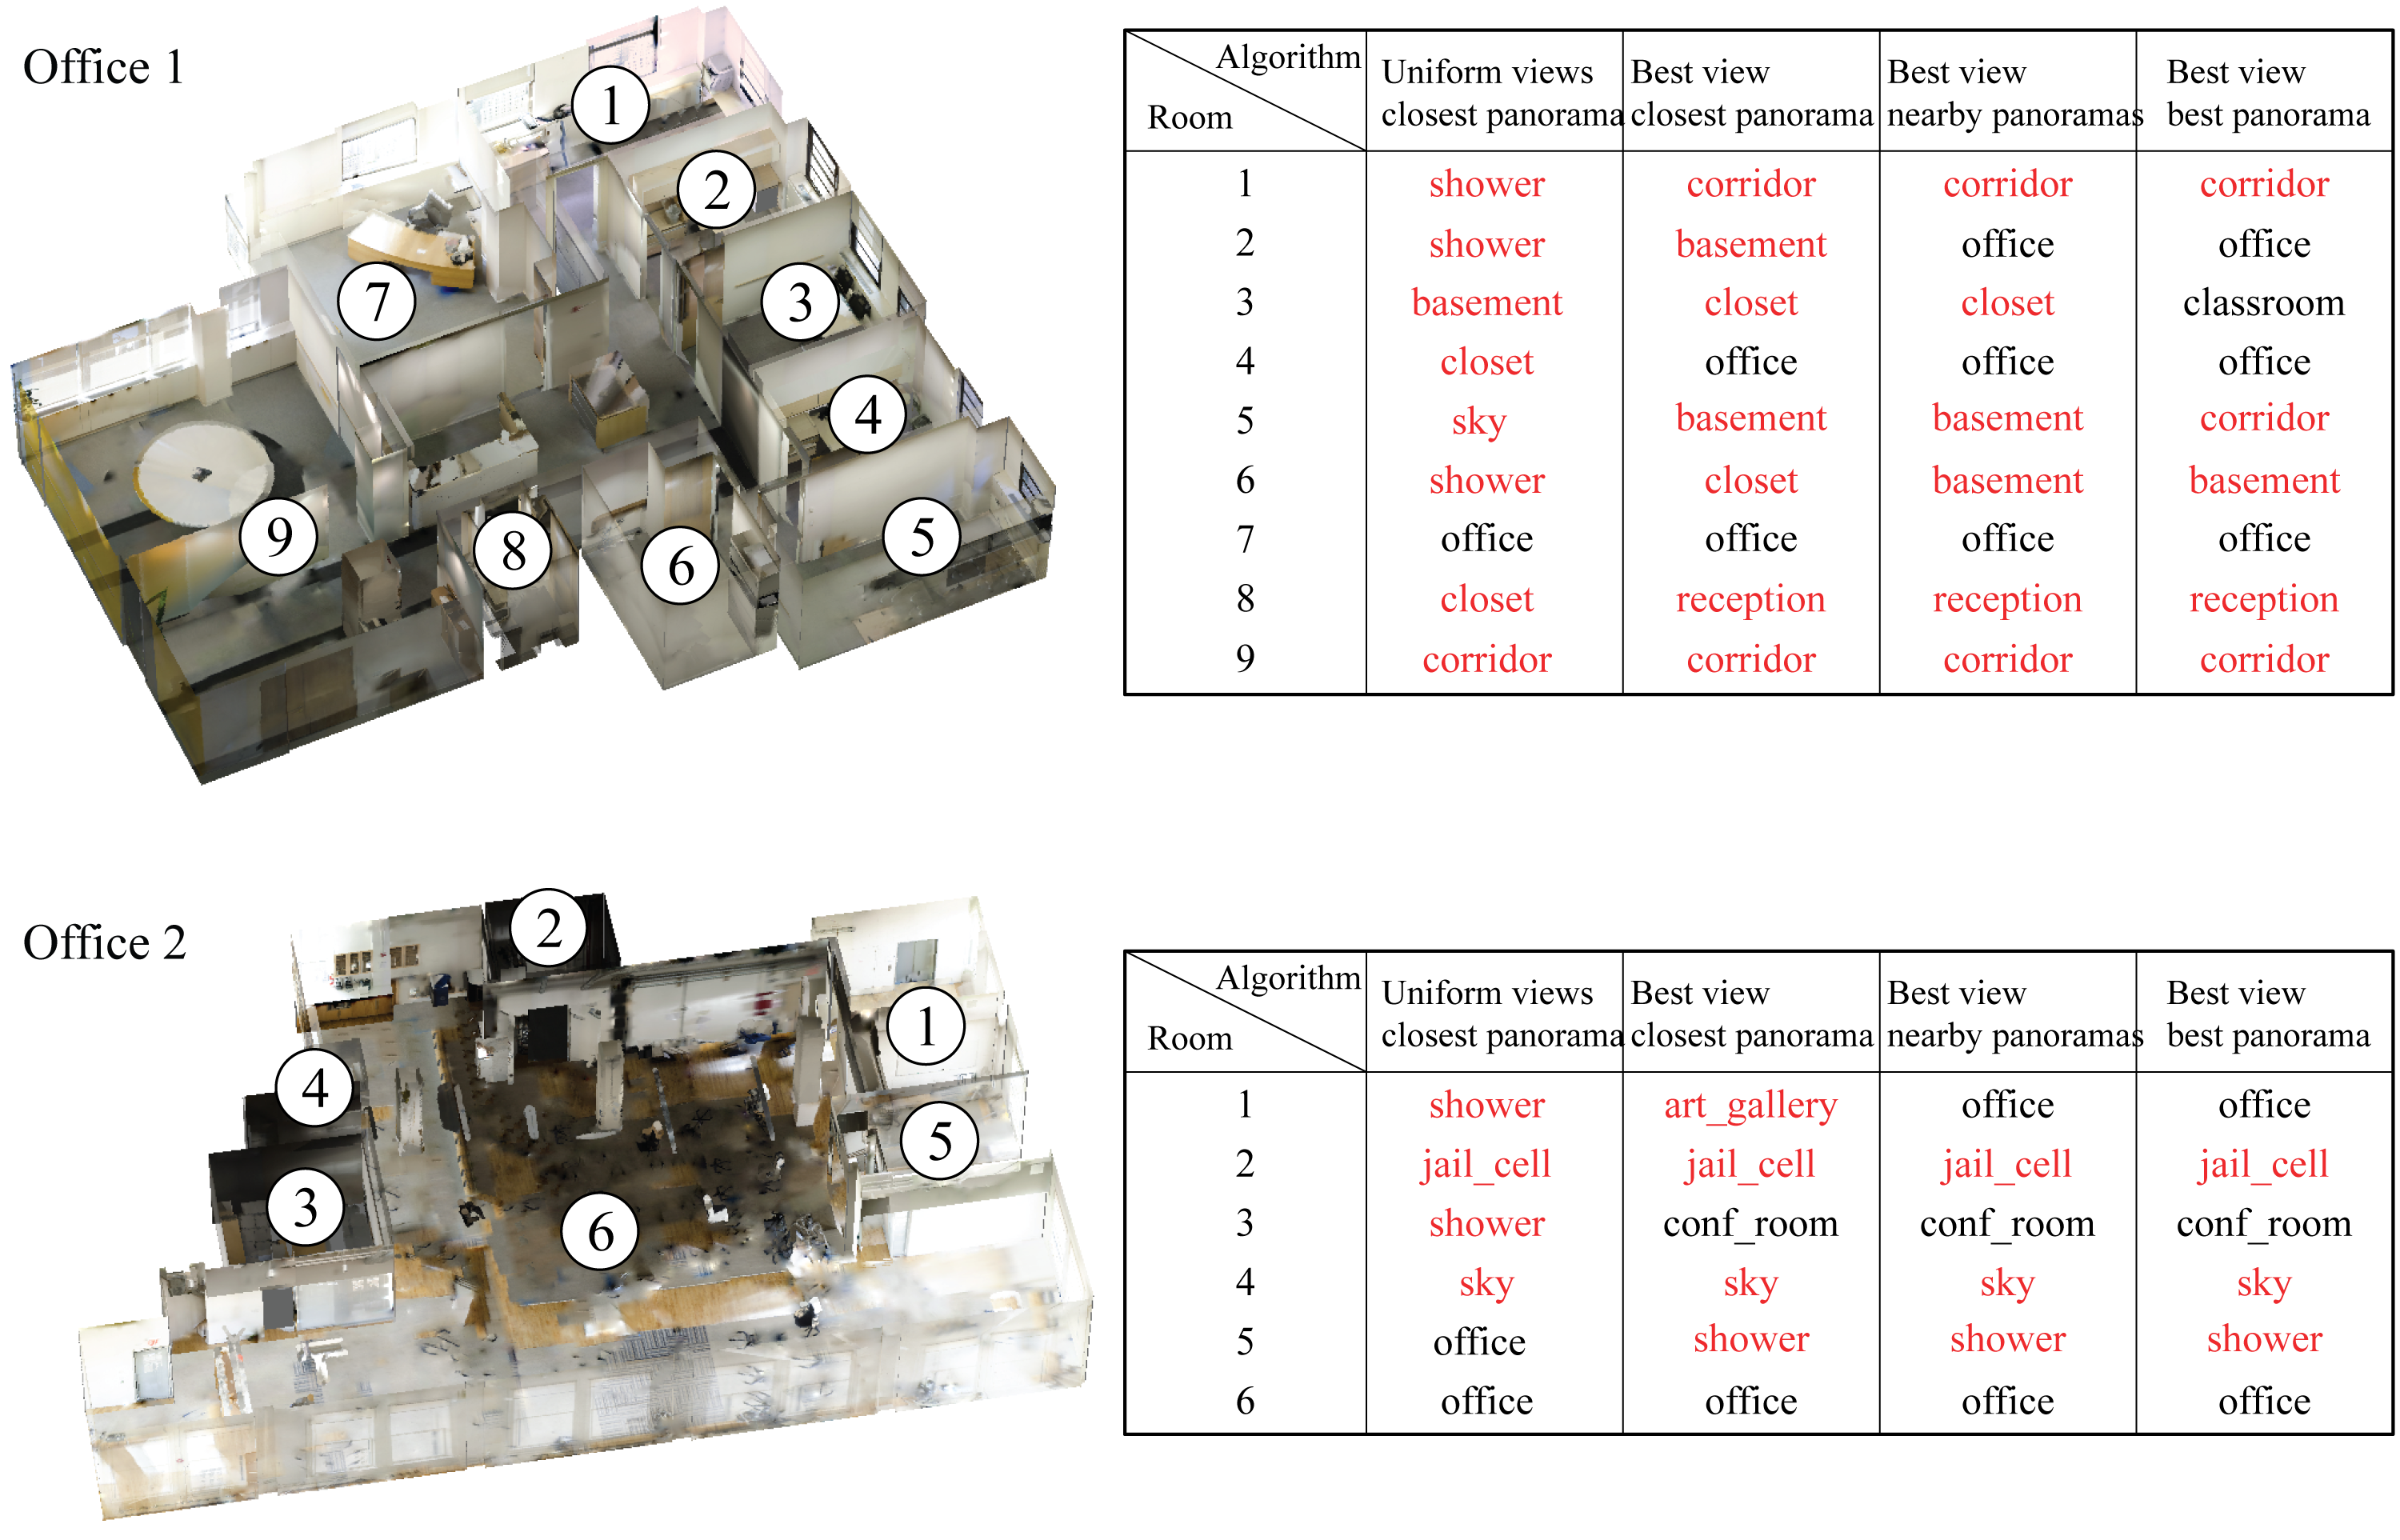
\includegraphics[width=\textwidth]{../figures/room_recognition_stats.png}
   \includegraphics[width=\textwidth]{../figures/room_recognition_stats_compressed.pdf}
  \caption{Continued.}
 \label{fig:room_recog1}
\end{figure*}

\clearpage
\begin{figure*}[!t]
  \centering
   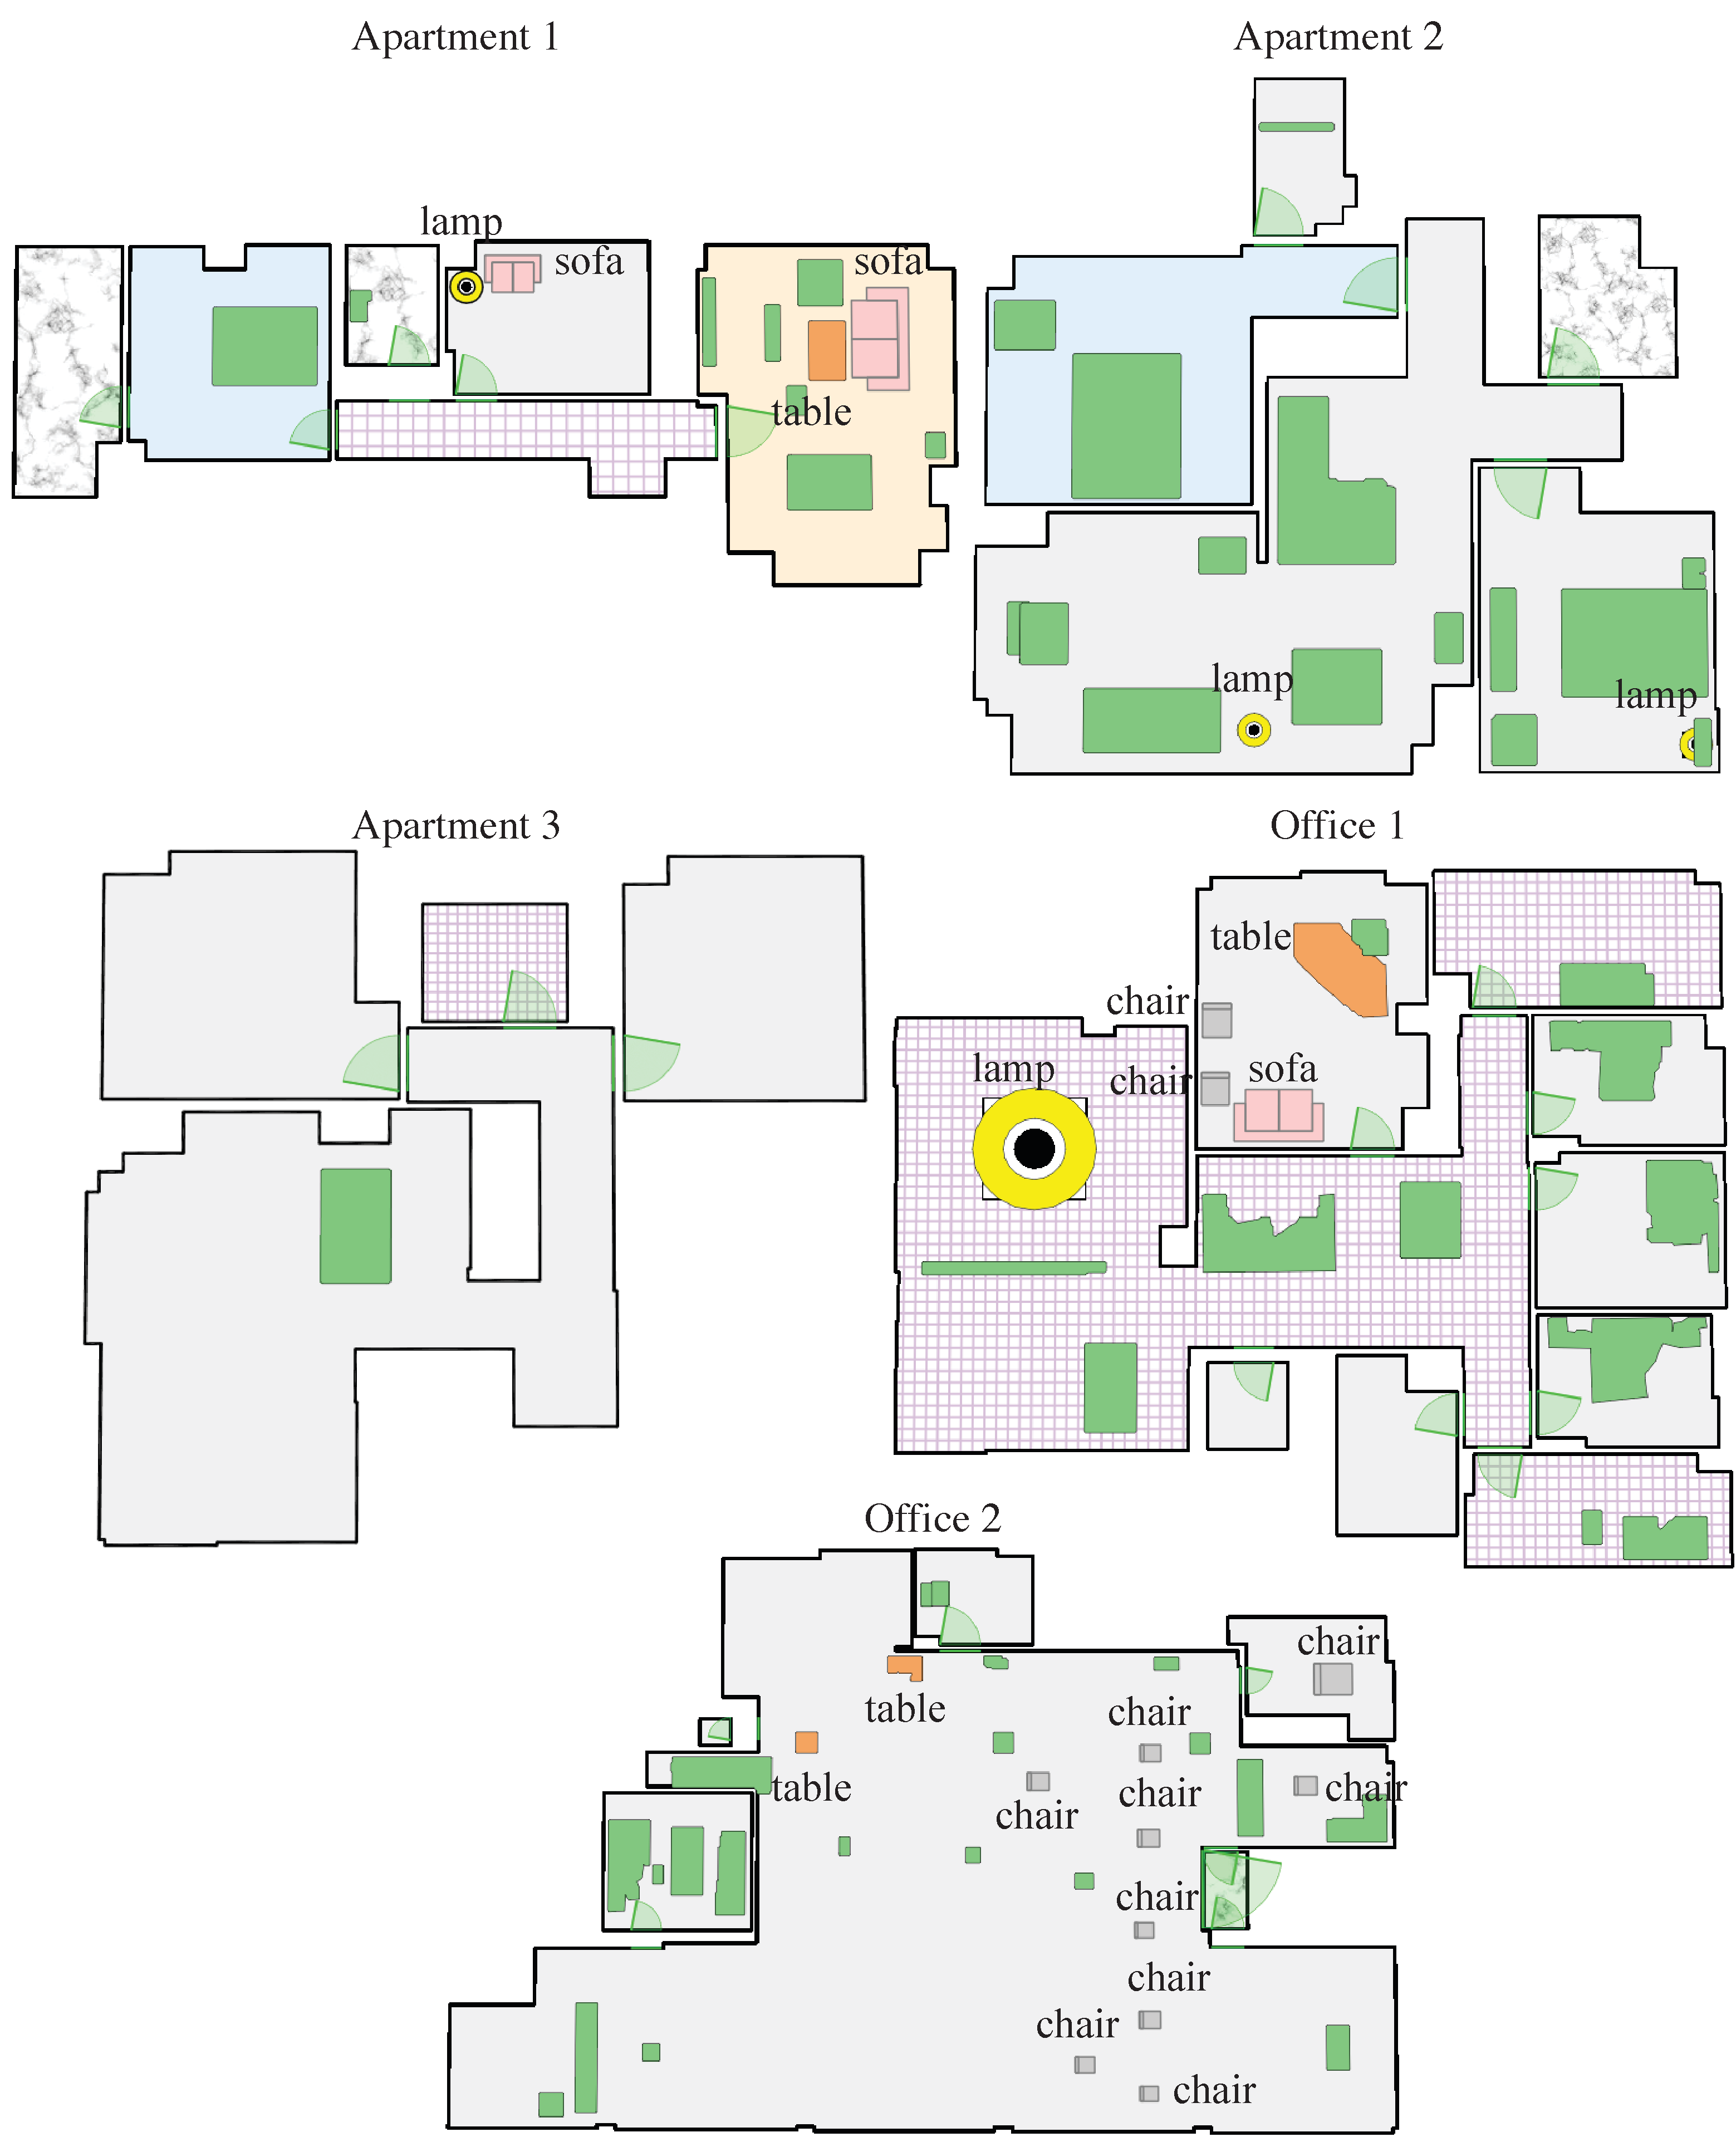
\includegraphics[width=\textwidth]{../figures/object_annotation.pdf}
  \caption{The object annotations turn out to be much more difficult
  than the room annotation. No texts are shown if an annotation cannot
  be associated. The segmentation results are good for major objects,
  and annotations, once obtained, are usually accurate.  However, most
  objects are missing annotations, especially in cluttered and small
  indoor rooms. A lot more improvements are to be made in this space.  }
  \label{fig:object_recog}
\end{figure*}

\clearpage
\begin{figure*}[!t]
  \centering
  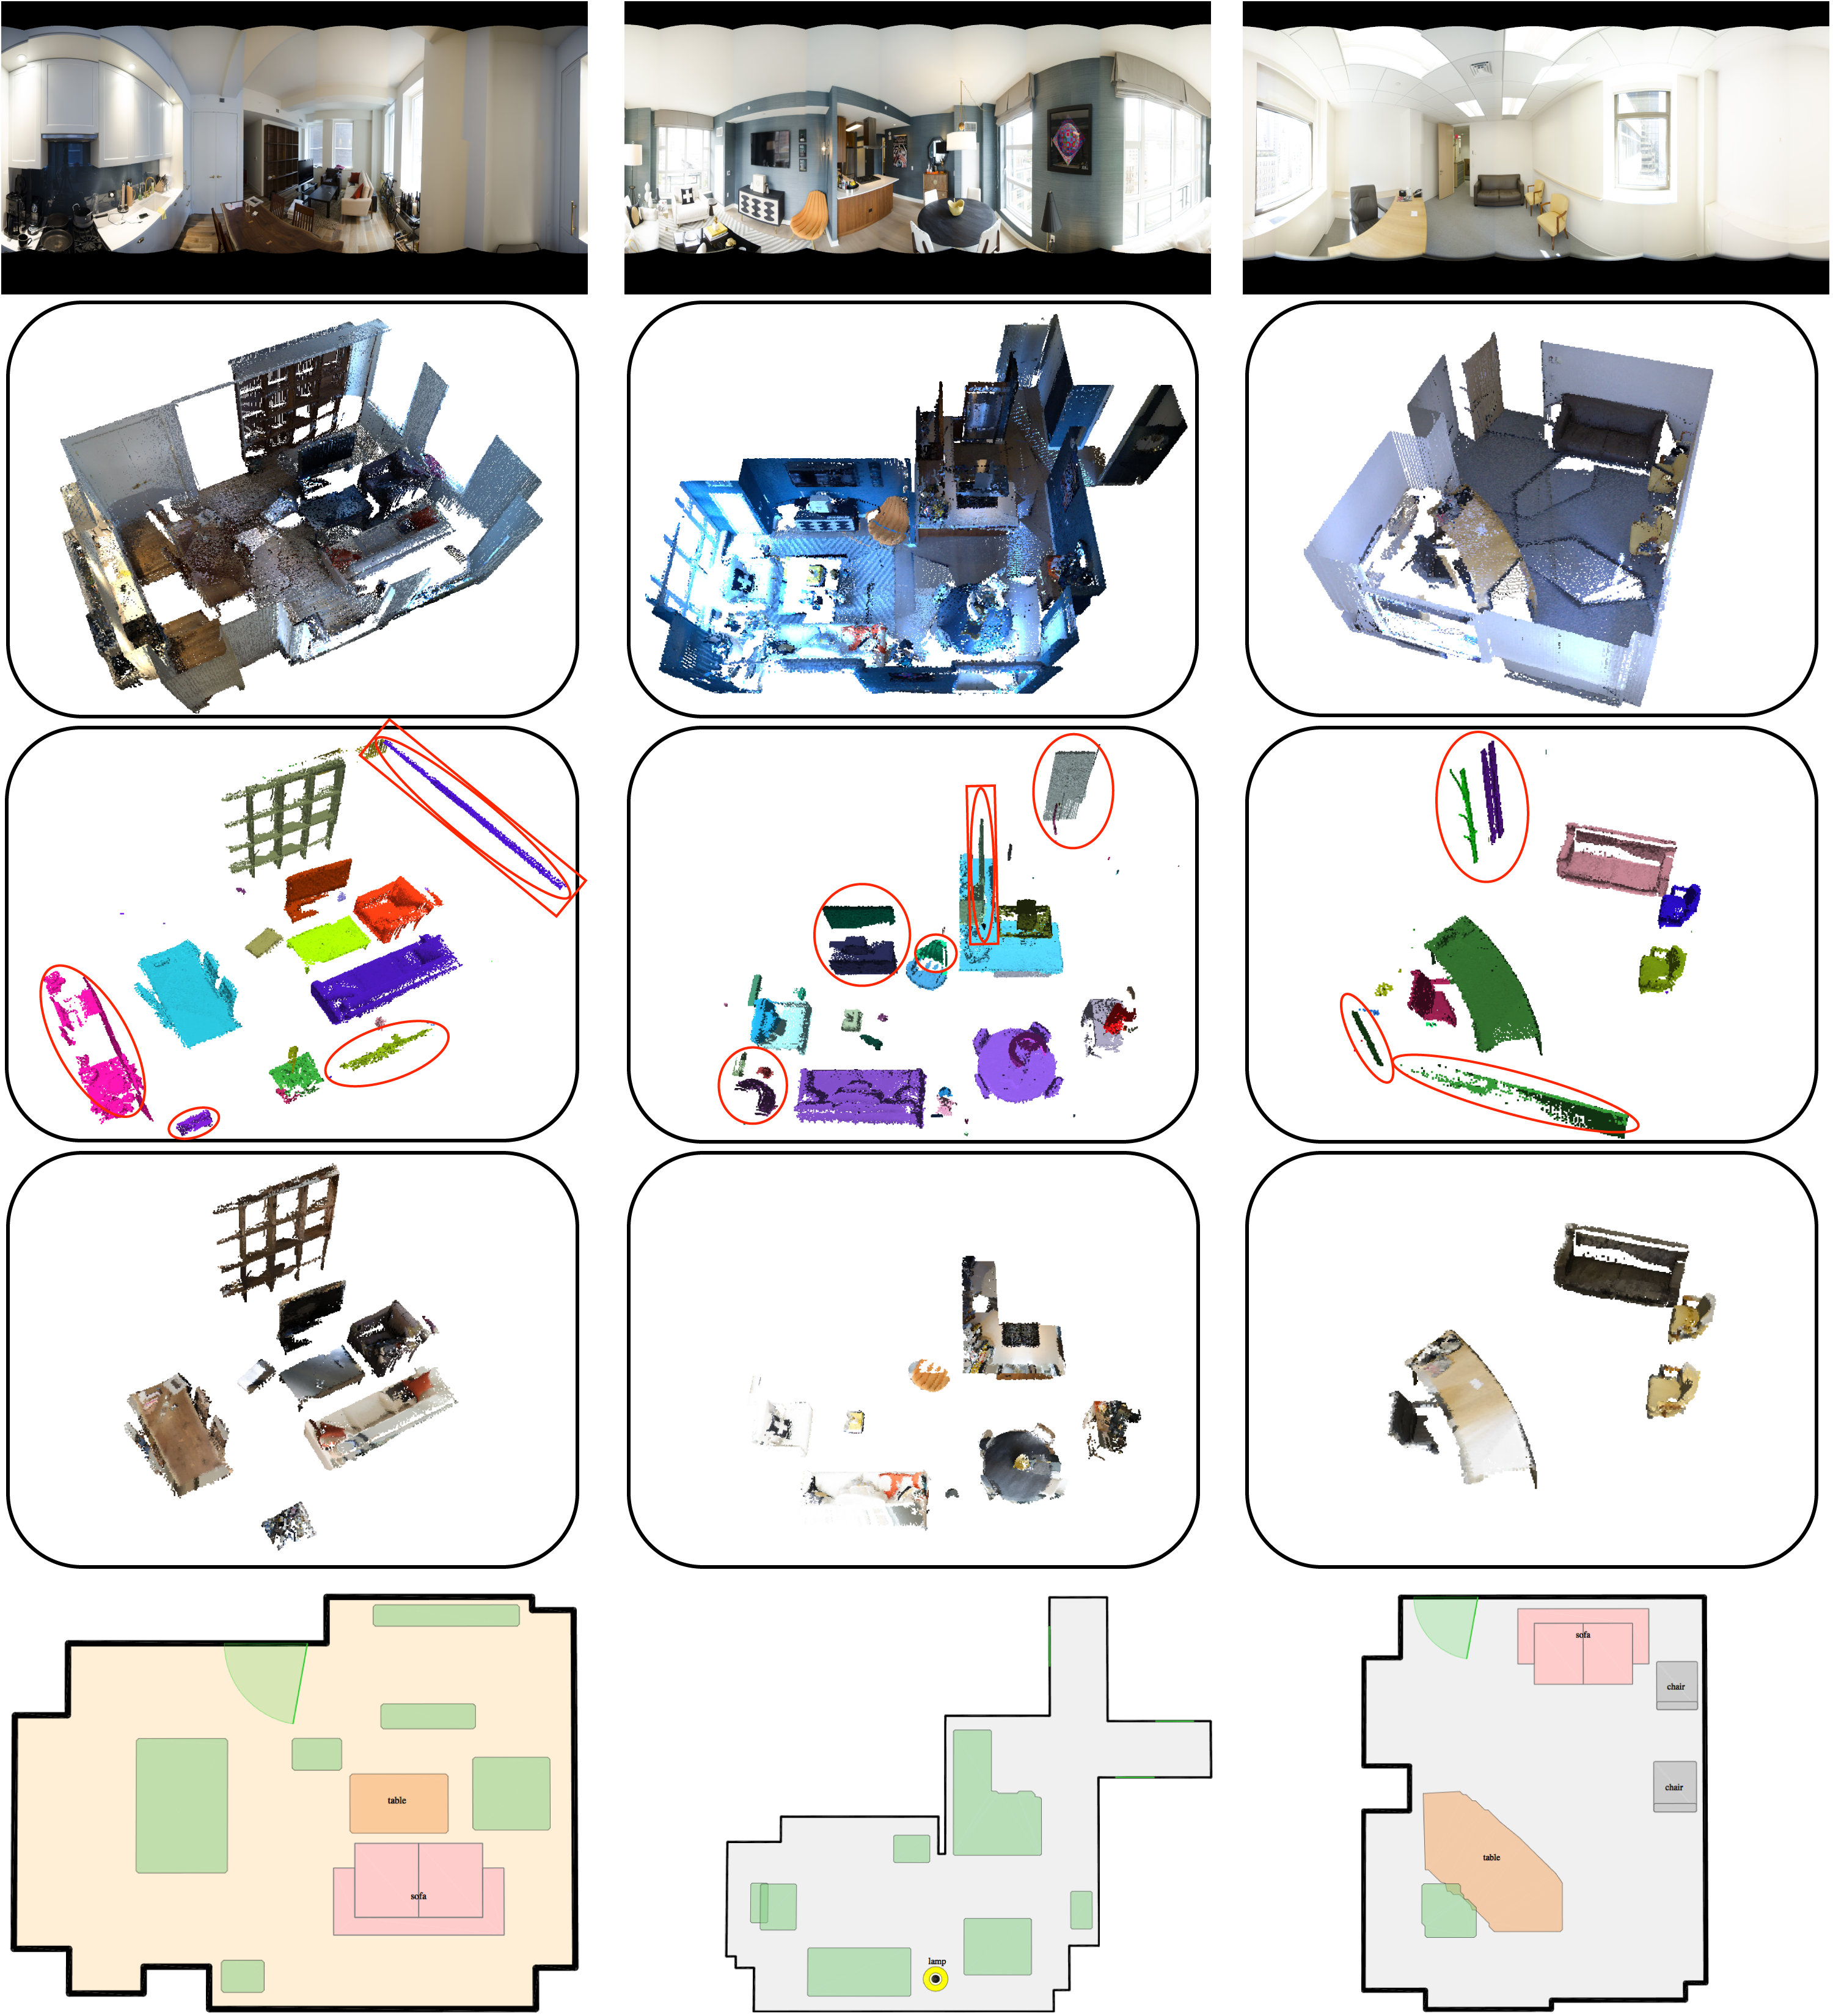
\includegraphics[width=\textwidth]{../figures/object_reconstruction.png}
%   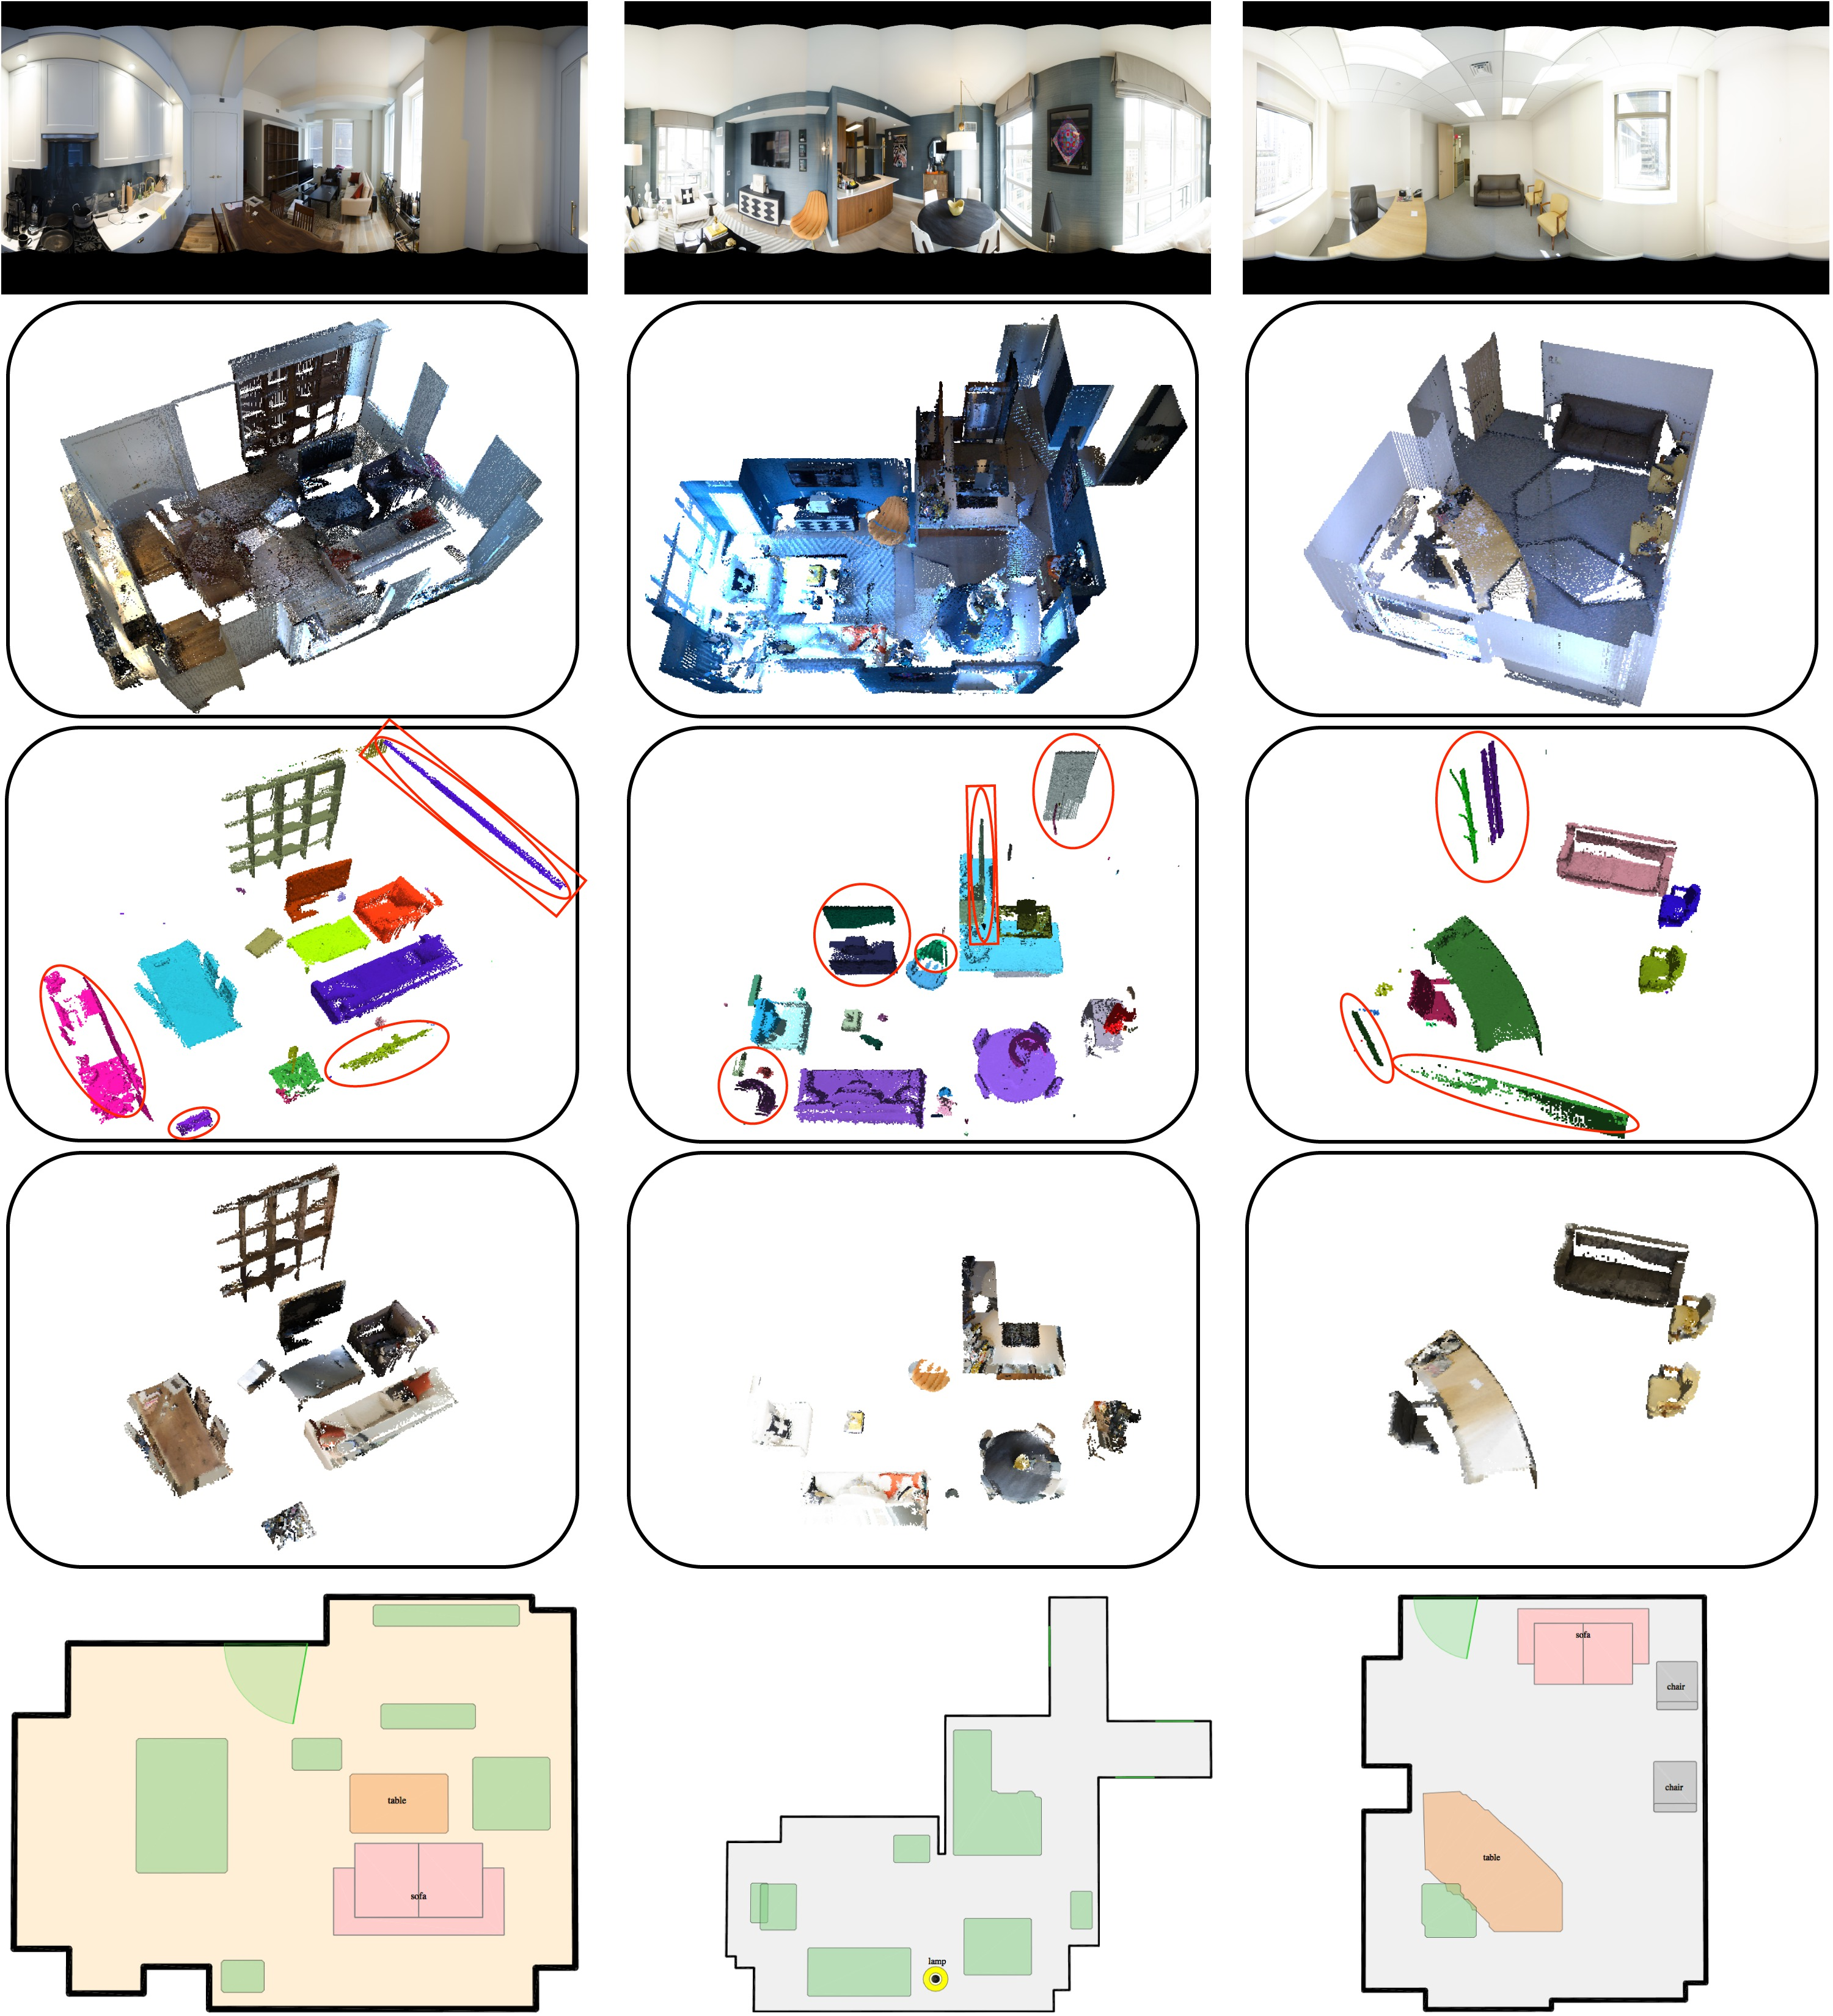
\includegraphics[width=\textwidth]{../figures/object_reconstruction.pdf}
  \caption{The figure illustrates our object reconstruction process for
  three rooms in our datasets.  From top to bottom: 1) a sample panorama
  image in the room; 2) the point-cloud in the room; 3) a point-cloud
  cluster for each object after removing points nearby the walls, the
  floors, or the ceilings; 4) point-cloud clusters after removing
  clusters that are too small or float in the air; and 5) the
 corresponding generated floorplan image in the room.
 % Object reconstruction pipeline. We want to reconstruction the
 %  objects in room shown in the first row. The second row shows all
 %  points inside the room. The third row shows the result after removing
 %  room structure(floors, ceilings and walls) and performing clustering
 %  to the remaining points. These segmentation results contain some
 %  floating objects(marked with green circles) and objects that are near
 %  room structure(marked with red circles), which can be replaced by room
 %  details. The fourth row shows the results after removing circled
 %  objects and small noisy objects, plus assigning colors from
 %  panoramas. The last rows shows the contours of objects from floorplan
 %view.}
 }
 \label{fig:objectreconstruction}
\end{figure*}

\clearpage
\begin{figure*}[!t]
  \centering
  \includegraphics[width=0.9\textwidth]{../figures/graphnew.pdf}
%   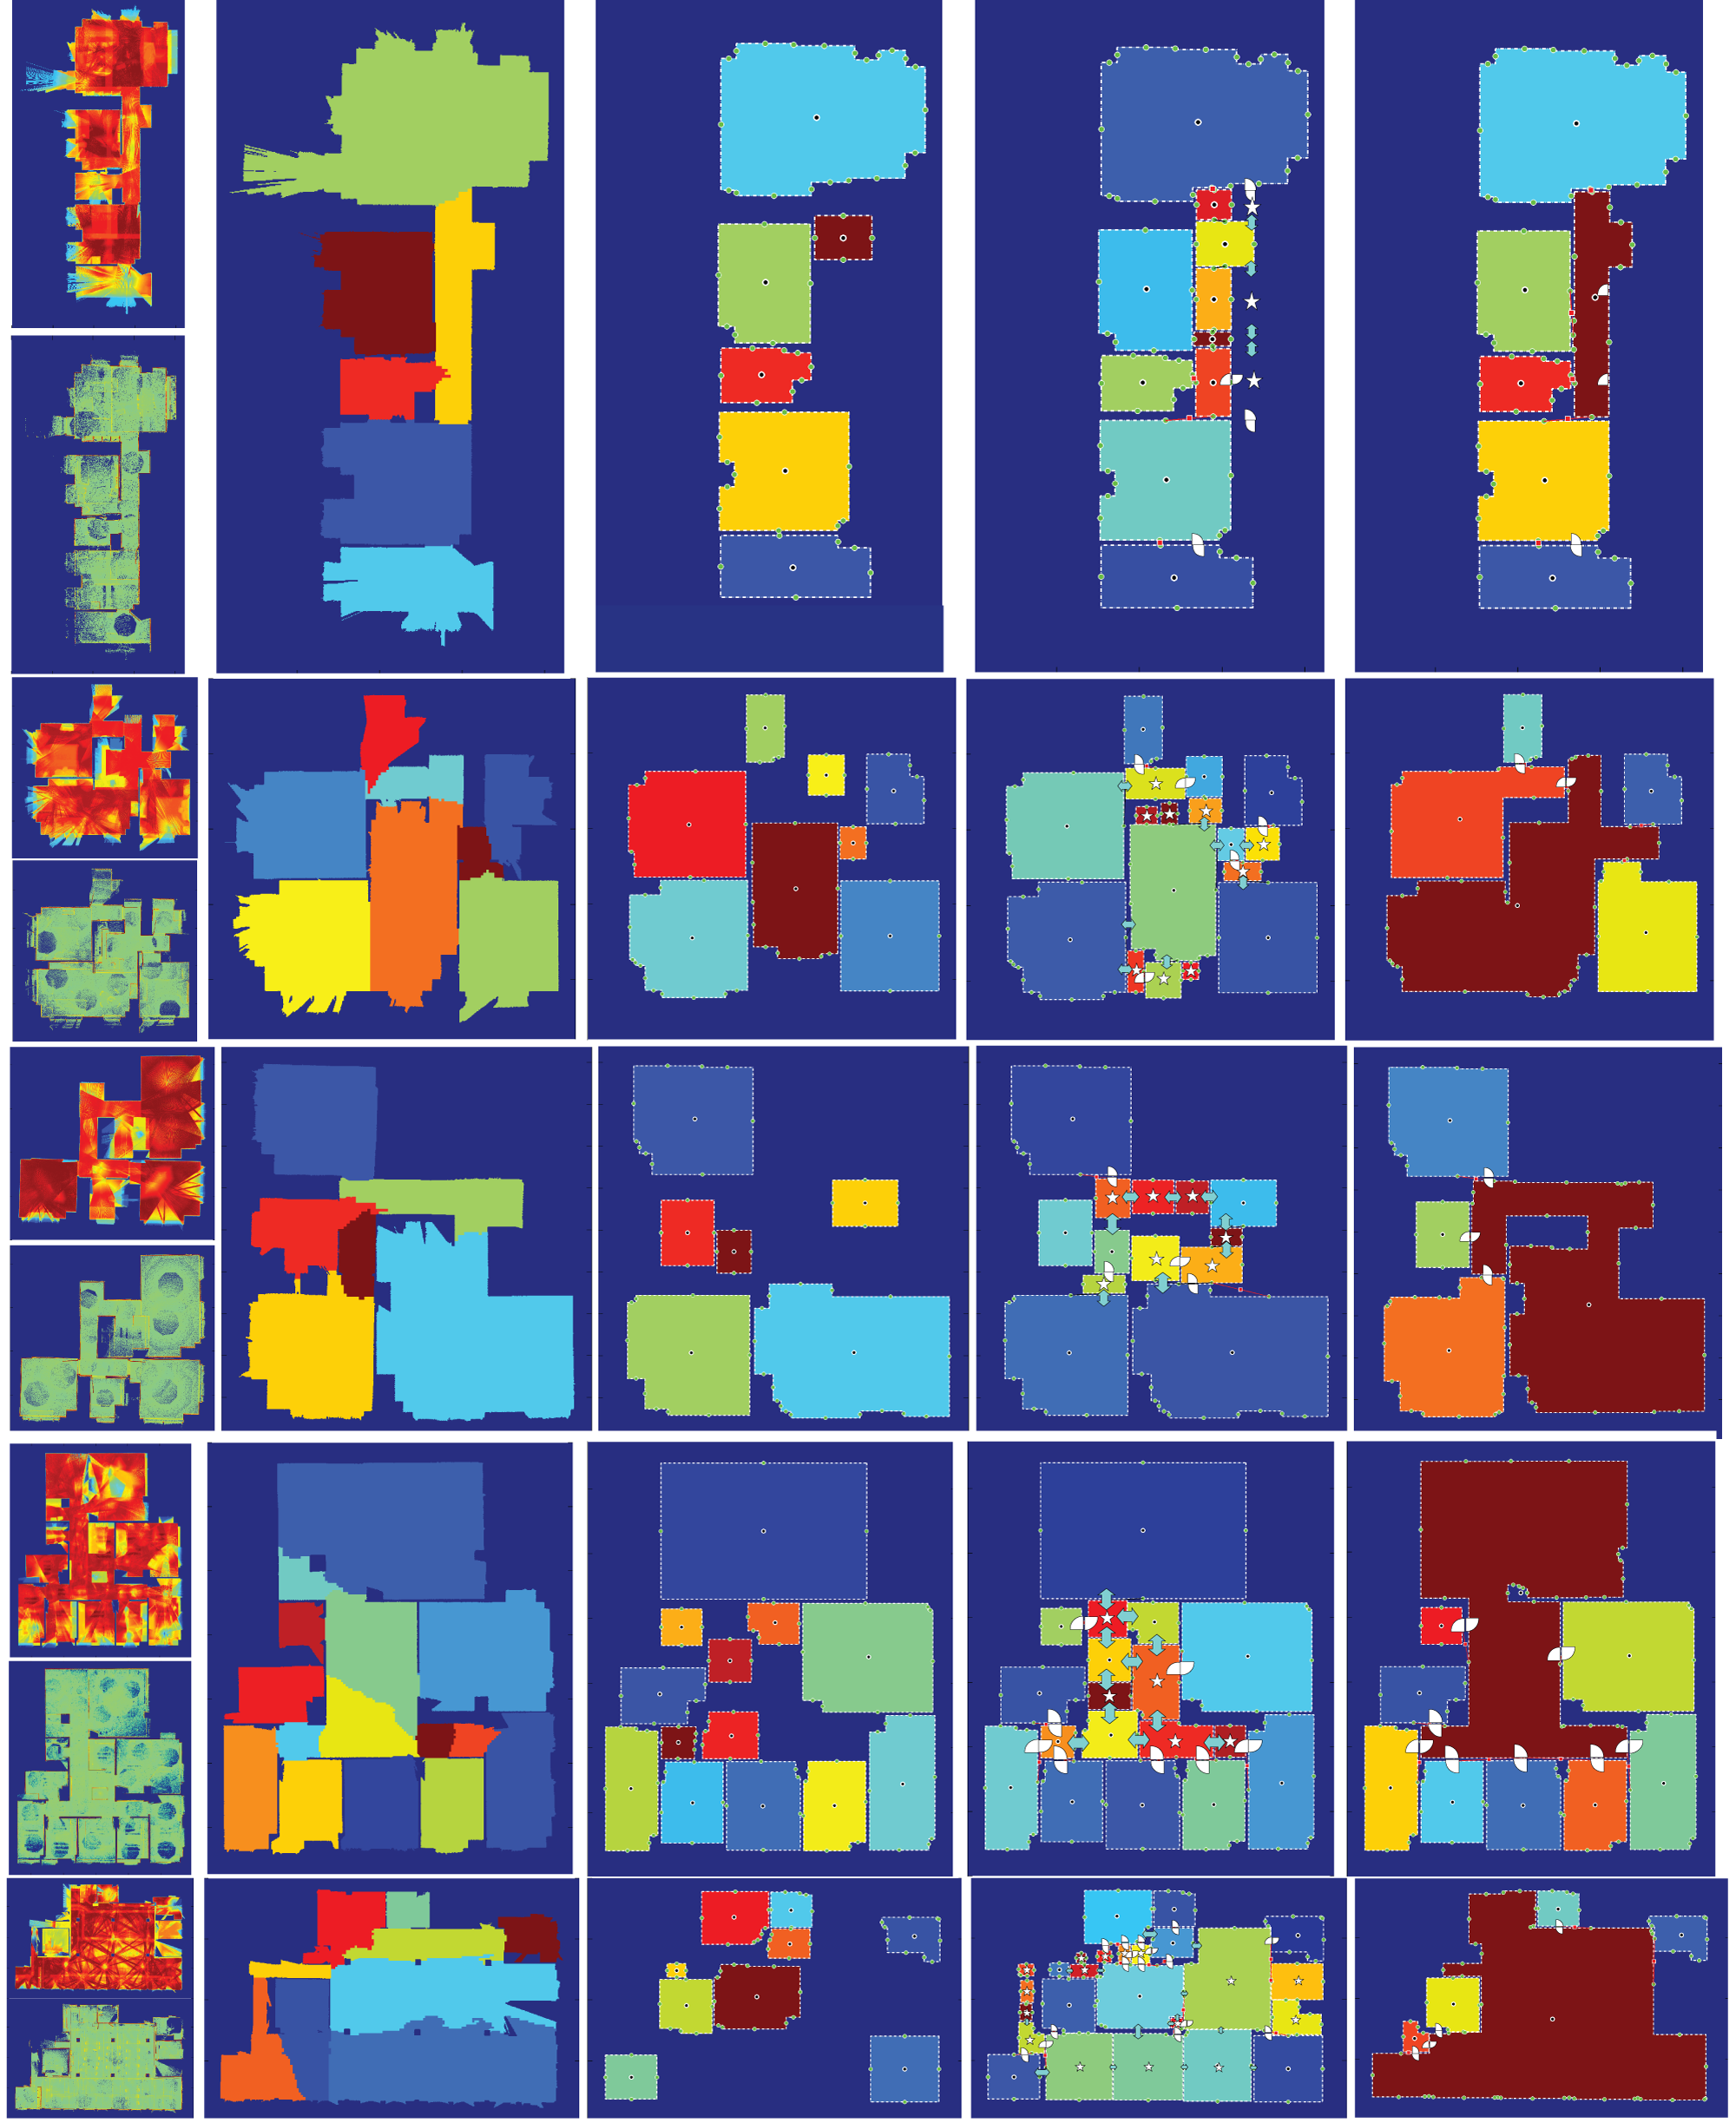
\includegraphics[width=0.9\textwidth]{../figures/graph_steps.png}
  \caption{Starting from the generation of the free-space end point
  evidence (left), we perform the room-segmentation and reconstruction
  (2-nd and 3-rd column).  More rooms are added and the room connection
  types are classified (4-th column). The white icon represents the
  ``door'', while the blue icon represents the ``merge'' classification.
  We finally get the structured graph representation as shown in the
  last column. Here we only show the spatial relationships for
  simplicity. }
\end{figure*}

\clearpage




\section{Structure graph - theory}

The main paper provides the key ideas behind the structured modeling
formulation. The supplementary material presents the complete
mathematical definition, constraints, and proofs.
% rties, and constraints of the structure
% graph.  We will prove that meshes compiled from the structure graph in
% various levels of details are manifolds, and show that our indoor
% structure grammar and the associated reconstruction algorithms satisfy
% the constraints.

\subsection{Definitions}

Let $v$ denote a node in a structure graph and its associated geometry
with abuse of notation. We consider a 2D surface representation of $v$,
where $\Gamma(v)$ denotes its boundary.
%
The graph has directed and undirected edges. The {\em attachment}
edges in the main paper are ignored in this analysis, as they do not exhibit
geometric constraints across elements (except for intersections, which
will be discussed later).
%Level-of-details edges are directed, while boundary edges are not.
%
% We use $\mathcal{E}_L$ and $\mathcal{E}_B$ to denote the
% level-of-details and the boundary edges, respectively. $\mathcal{E}_L$
% are directed, while $\mathcal{E}_B$ are not.

\begin{wrapfigure}{r}{0.35\columnwidth}
  \includegraphics[width=0.34\columnwidth]{../figures/graph_proof.pdf}
 \caption{Three types of connected nodes: $V^P_1$, $V^N_j$,
 and $V^C_k$.}
\end{wrapfigure}
The right figure shows that potential connections at a node are a parent
$V^P_1$, neighbors $V^N_j$, and children $V^C_k$.
We define
\begin{eqnarray*}
\Gamma(e^P_1) &=& \Gamma(v)\cap \Gamma(v^P_1), \nonumber\\
\Gamma(e^C_k) &=& \Gamma(v)\cap \Gamma(v^C_k), \nonumber
% \Gamma(e^N_j) &=& \Gamma(v^N_j) \cap \left[\Gamma(v) \setminus
%                                     \Gamma(e^P_1)\right] \nonumber
\end{eqnarray*}
Edge $\Gamma(e^P_1)$ conveys a part of the boundary condition of $v^P_1$
that must be satisfied by $v$ for manifold-ness. The same is true for
$\Gamma(e^C_k)$.  The boundary associated with an edge must not be
$\emptyset$, otherwise the edge should not be connected. $\Gamma(e^N_j)$
conveys the surface boundary where the two incident nodes must match
exactly for manifold-ness. Its definition is not the simple intersection
and will be later derived from the constraint.
%
We use $\mathcal{P}$(arents), $\mathcal{N}$(eighbors), and
$\mathcal{C}$(hildren) to denote a set of nodes that are connected by
$e^P_1$, $e^N_j$, and $e^C_k$, respectively. Note that we will have a
constraint not to allow multiple parents, and hence $P$ can have at most
one node.
%
%$e^B_{ij}$ denotes a boundary connecting $n_i$ and $n_j$. $e^L_{ij}$ is
%a directed edge from $n_i$ to $n_j$.
%
%$\Gamma(n_i)$ and $\Gamma(n_j)$ have an overlap, where the geometries
%exactly match.

\subsection{Constraints}
%\end{eqnarray*}
% Similarly, given a level-of-details edge $e^L_{ij}$ from $n_i$ to $n_j$, their
% common surface boundary is denoted as
% %\begin{eqnarray*}
%  $\Gamma(e^L_{ij}) = \Gamma(n_i) \cap \Gamma(n_j).$
% %\end{eqnarray*}
%
\begin{enumerate}[itemsep=0mm]
 \item[C1:] The geometry $v$ is a single connected component.
 \item[C2:] The geometry $\bigcup_k v^C_k$ is a single connected
            component, if $\mathcal{C}\ne \emptyset$.
 \item[C3:] $\Gamma(v) = \Gamma(e^P_1) \cup
            \left[\bigcup_j \Gamma(e^N_j)\right]$ if
            $\mathcal{P}\ne \emptyset$  or $\mathcal{N} \ne \emptyset$.\\
  $\{\Gamma(e^P_1), \Gamma(e^N_1), \Gamma(^N_2) \cdots \}$ are mutually
            exclusive.
            %do not have a common boundary interval.
 \item[C4:] $\Gamma(v) = \bigcup_k \Gamma(e^C_k)\quad $ if $\mathcal{C} \ne \emptyset.$\\
            $\{\Gamma(e^C_1), \Gamma(e^C_2) \cdots\}$ are mutually exclusive.
            %do not have a common boundary interval.
 \item[C5:] The graph is acyclic with respect to the directed edges.
 \item[C6:] A node cannot have multiple parents.
\end{enumerate}

The structure graph must satisfy these constraints.
C2 states that the surface formed by the children must be a single connected
component. This appears restrictive but is not.
%In case, one needs to model multiple connected components coming out
%from a node,
For modeling multiple connected components from a single surface, one
should first split the domain, then add a component to each sub-domain.
% then add a node to each split region.
%
C3 states that the boundary condition of a node is satisfied by
its neighbors and parent.
%
C4 states that the boundary condition of $v$ is propagated to its
children.
%In other words, the boundary condition is satisfied if the
%condition is satisfied at its children.

\subsection{Proofs}

\begin{lemma}\label{lemma1}
$\Gamma(e^N_j) = \Gamma(v^N_j) \cap \left[\Gamma(v) \setminus
                                     \Gamma(e^P_1)\right]$.
\end{lemma}

\begin{proof}
C3 guarantees no intersection between $\Gamma(e^P_1)$ and
 $\Gamma(e^N_j)$. Therefore, the first line of C3 can be converted to
\begin{eqnarray*}
 \Gamma(v) \setminus \Gamma(e^P_1) = \bigcup_j \Gamma(e^N_j).
\end{eqnarray*}
Again \{$\Gamma(e^N_j)$\} are mutually exclusive, and
\begin{eqnarray*}
 \Gamma(e^N_j)\cap \left[\Gamma(v) \setminus \Gamma(e^P_1)\right] &=&  \Gamma(e^N_j)\cap
  \left[\bigcup_j \Gamma(e^N_j)\right], \nonumber \\
 \Gamma(e^N_j)\cap \left[\Gamma(v) \setminus \Gamma(e^P_1)\right] &=&  \Gamma(e^N_j).\nonumber
 \end{eqnarray*}
\end{proof}
 
Lemma~\ref{lemma1} implies that only the boundary condition that has not
been satisfied by the parent should be satisfied by the neighbors.

\begin{lemma}\label{lemma2}
The nodes in $\mathcal{C}$ form a single connected component with respect
to the undirected edges.
\end{lemma}
 
\begin{proof}
Suppose $\mathcal{C}$ forms multiple connected components with respect
to the undirected edges. Due to C2, there must be a pair of nodes ($v$,
$v^N_j$) that shares the parent, are physically connected, but are not
connected by $e^N_j$, that is, $\Gamma(e^N_j) = \emptyset$. We use
$\gamma$ to denote the physical surface boundary shared by these two
nodes:
\begin{eqnarray*}
 \gamma = \Gamma(v^N_j) \cap \Gamma(v).
\end{eqnarray*}
From Lemma~\ref{lemma1}, the following holds
\begin{eqnarray*}
 \Gamma(v^N_j) \cap \left[\Gamma(v) \setminus
                     \Gamma(e^P_1)\right] = \emptyset.
\end{eqnarray*}
Since $v$ and $v^N_j$ has a common boundary $\gamma$, $\Gamma(e^P_1)$
 must contain $\gamma$ for the above to hold.
 \begin{eqnarray*}
 \gamma \subseteq \Gamma(e^P_1).
\end{eqnarray*}
% 
$v$ and $v^N_j$ are interchangeable, and shares the parent. Therefore,
this relationship is also true for another child of $v^P_1$.
However, this violates the mutual exclusiveness in C4.
\end{proof}

Note that C2 states that $\mathcal{C}$ forms a single connected
component in terms of its geometry. However, this does not provide a
proof, as $\Gamma(e^N_j)$ can be $\emptyset$. Therefore, the above
derivation completes the proof. Now, let us define that a {\it leaf
node} does not have any out-going edge for the next lemma.

\begin{lemma}\label{lemma3} 
Given a structure graph, geometries at all the leaf nodes form a
manifold,
\end{lemma}

\begin{proof}
Given geometries at all the leaf nodes, we prove that the boundary
conditions are satisfied at every node by induction. Let us first
calculate the ``distance'' from the leaf-node as the fewest number of
directed edges to reach any leaf. The induction is performed based on
these distances.

First, at a leaf node, a geometry is created, and C3 ensures that its
boundary conditions are satisfied at its boundary edges $\{e^N_j\}$ and
the in-coming edge $e^P_1$.
%
Second, suppose boundary conditions $\Gamma(v)$ at a node $v$ are
satisfied where the distances are less than or equal to $k$.  Given a
node whose distance is $k+1$, the boundary conditions at the out-going
directed edges are satisfied, because the edges point to the nodes whose
distances are at most $k$. C4 ensures that the entire boundary of $v$ is
generated by its out-going edges, all of which are now satisfied.  Then, C3
again confirms that the boundary conditions are satisfied at its
boundary and in-coming edges further up the tree.
%
By induction, the boundary conditions are satisfied at every node.
\end{proof}

Our mesh compilation process generates a mesh after pruning an arbitrary
set of nodes. This pruning operation must not leave any dangling
boundary edges.

\begin{lemma}\label{lemma4}
The structure graph group (a set of valid structure graphs) is closed
 under the pruning operation.
\end{lemma}

\begin{proof}
 We will check that every constraint is satisfied after any pruning
 operation.
\begin{enumerate}[itemsep=0mm]
 \item[C1:] Independent of the pruning.
 \item[C2:] Lemma~\ref{lemma2} shows that all the children nodes must be pruned
 ($\mathcal{C}$ becomes $\emptyset$) or stay connected ($\mathcal{C}$
 does not change).
 \item[C3:] It suffices to prove for a node $v$ that has not been
            pruned. Since
            no dangling boundary edge remains, all the neighbor nodes $v^N_j$
            should also stay in the graph. $v^P_1$ is a parent of $v$ and not
            pruned. Therefore, the equality stay unchanged.
            Mutual exclusiveness is independent of the pruning.
 \item[C4:] Due to Lemma~\ref{lemma2}, all the children nodes must stay or be
            pruned. Therefore, either the equality does not change or
            $\mathcal{C}$ becomes $\emptyset$.
            Mutual exclusiveness is independent of the pruning.
 \item[C5:] The graph loses connections by pruning, and is still acyclic.
 \item[C6:] Pruning will not add new parents.
\end{enumerate}
\end{proof}

\begin{theorem}
 The structure graph produces a manifold-mesh after dropping an
 arbitrary set of nodes, as long as no dangling boundary edges remain.
\end{theorem}

\begin{proof}
 Lemma~\ref{lemma3} and Lemma~\ref{lemma4} prove.
\end{proof}
 

% The second constraint ensures that the boundary condition is propagated
% to the children properly.
% \begin{eqnarray*}
%  \forall n_j \in C(n_i) \quad \forall n_k (\ne n_j) \in C(n_i), \quad
%   \Gamma(E^L_{ij}) \cap \Gamma(E^L_{ik}) = \emptyset.
% \end{eqnarray*}
% $C(n_i)$ denotes a set of children nodes of $n_i$.
%  
% $N_B(n_i)$ denotes a set of nodes that are connected to $n_i$ by the
% boundary edges. $N_L^I(n_i)$ (resp. $N_L^O(n_i)$) denotes a set of in-coming
% (resp. out-going) nodes that are connected to $n_i$ by the
% level-of-details edges.
%
% The first constraint
% ensures that the boundary condition of a node is satisfied exactly by
% the union of $N_B(n_i)$ and $N_L(n_i)$
%
% %
% Let $C(n_i)$ denote a set of child nodes that are connected from $n_i$
% by the level-of-detail edges. The boundary condition $\Gamma(n_i)$
% must be also satisfied by the children $C(n_i)$ as a whole. Let
%
% The structure graph is flexible, but must satisfy the following
% constraint at every node. The boundary condition at every node $n_i$
% must be satisfied by its parent if exists and its boundary edges:
%
% $\mathcal{E_L}$ are directed edges. 
%
% are directed edges, while the
% other two are undirected edges. $\mathcal{E_A}$ does not exhibit
% geometric constraints, and is ignored in our analysis here.


\subsection{Practical considerations}
It is easy to verify that our indoor structure grammar satisfies C5 and
C6. It is also easy to see that C1 and C2 can be easily checked or enforced.
The problems are C3 and C4,
%The structure graph requires the six constraints (C1 - C6) to be
%satisfied during the reconstruction process. The most challenging
% constraints are C3 and C5,
which impose non-trivial boundary conditions.  The key observation is
that the constraints act only on the surface boundaries. Therefore, our
approach is to first fix the boundaries of each node to satisfy the
constraints, then perform reconstruction algorithms subject to the given
boundary conditions. This section shows that it is relatively
straightforward to enforce these boundary conditions for each of the
major geometric representations.

The first scenario is the 2D offset-map reconstruction on a quad patch
(\eg, wall detail reconstruction), where the boundary condition is at
the boundary of the quad. We simply fix the depth values along the
boundary, then the final 2D surface is guaranteed to match the specified
boundary.

The second case is the volumetric scalar field followed by the Marching
Cube algorithm for the mesh generation. Given the boundary condition, we
know that the nearby space (voxels) must be either interior of exterior,
which can be enforced by fixing the scalar values at the corresponding
voxels~\cite{shan2014occluding}. The same goes for the point-cloud
reconstruction.

Intersections in addition to the boundary condition can also be enforced
in a similar manner. For an offset-map estimation algorithm, for
example, infinite data terms can be used to avoid the reconstruction to
go inside the interiors of the other geometries. The same goes for the
volumetric scalar field and the point-cloud reconstruction, where the
voxel values can be fixed inside the interiors of the other geometries.
% a configuration with intersections with
% other geometries.  The surface extraction step from the voxels can
% similarly use hard constraints to avoid self-intersections. For example,
% assigning the infinite penalty for a voxel to become scene exterior, if
% it sits inside an existing geometry.
In our experiments, we do not enforce the intersection check in the
reconstruction algorithms, as self-intersections are rare in
practice. Furthermore, even if there exist, they do not pose problems to
any of our applications.



%either, as the point-clouds suffice or are better for the main
%visualization applications. and geometry suffers.



%talk about the fact that objects are points, and we did not pay
%attention to meshing much.

Lastly, point-clouds are not converted to meshes for objects in our
experiments for two reasons. First, point-clouds suffice for the
visualization applications. Second, proper meshing of complex objects in
the indoor scenes is a challenging problem by itself with very active
on-going research. Note that our framework allows one to use any object
reconstruction algorithm, even different algorithms for different
object types, and we can easily exploit any other object reconstruction
algorithm as a component.



\section{Remaining structure grammar}

This section presents the three remaining grammar rules.

\mysubsubsection{Room merging} The rule takes two rooms and merges into
a single room node, while discarding all the details and doors in each
room (transformation). The room connection type must be
classified as ``merge''(pre-condition). The details of the connection
classification will be given below. Given a “merge” connection classification, we connect the core free-space regions of the two rooms and simply apply the room reconstruction rule. 

\mysubsubsection{Room addition} In the process of room reconstruction
and merging, the domain $\Psi$ for the room segmentation (Sect. 4.3 in
the main paper) may have a region that does not belong to any room. The
rule adds a new room node to a scene
%takes a scene with reconstructed rooms (pre-condition), then
(transformation). 
%
There are three pre-conditions. We identify the axis-aligned rectangle
with the most area inside such uncovered region. The first condition is
that the area of the rectangle is larger than $0.05$ times the average
room area.  The next two conditions prevents generating rooms outside
the windows, where 3D points suffer from strong structured noise.
%
Second, find the closest room from every pixel inside the
rectangle. There must be at least two rooms found.
% inside the rectangle.
Third, the sum of the point evidence inside the rectangle must not be
too small, in particular, more than half the sum of the free-space
evidence.
%
%When these conditions are met, we generate a room node, which will
%trigger a room reconstruction algorithm.

\mysubsubsection{Door addition} Given two rooms, whose connection type
is classified as ``door'' (pre-condition), a rectangular hole (\ie,
doorway) is created in each wall. The door geometry, consisting of four
planes connecting the two rectangular holes, is also created
(transformation). Since the wall geometry or the detailed wall geometry
are an 2D offset-map, it is easy to create a rectangular hole.


\mysubsubsection{Room connection classification}
\begin{figure}[!t]
	\begin{center}
		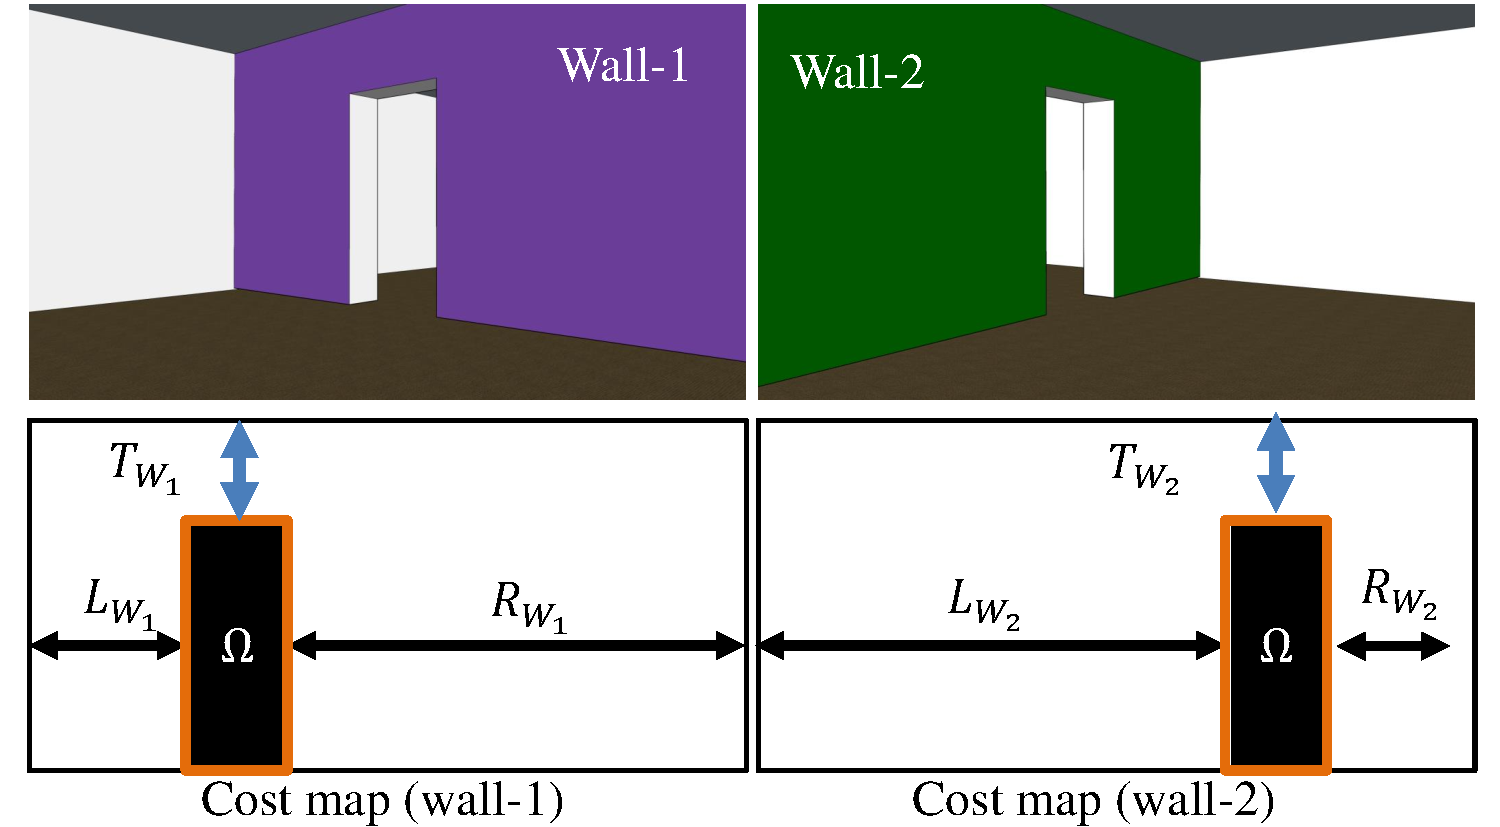
\includegraphics[width=85mm]{../figures/wallprofile.pdf}
	\end{center}
	\vspace{-0.2cm}
	\caption{Once the rectangle $\Omega$ is extracted, we compute
 the left, the right, and the top margins between the rectangle and the
 wall.}
% three distances for each wall independently, between the side of the rectangle and the side of the wall $L_W, R_W$, and the top of the rectangle and the ceiling.}
	\label{fig:wallprofile}
	\vspace{-0.25cm}
\end{figure}
\begin{figure}[!t]
	\begin{center}
         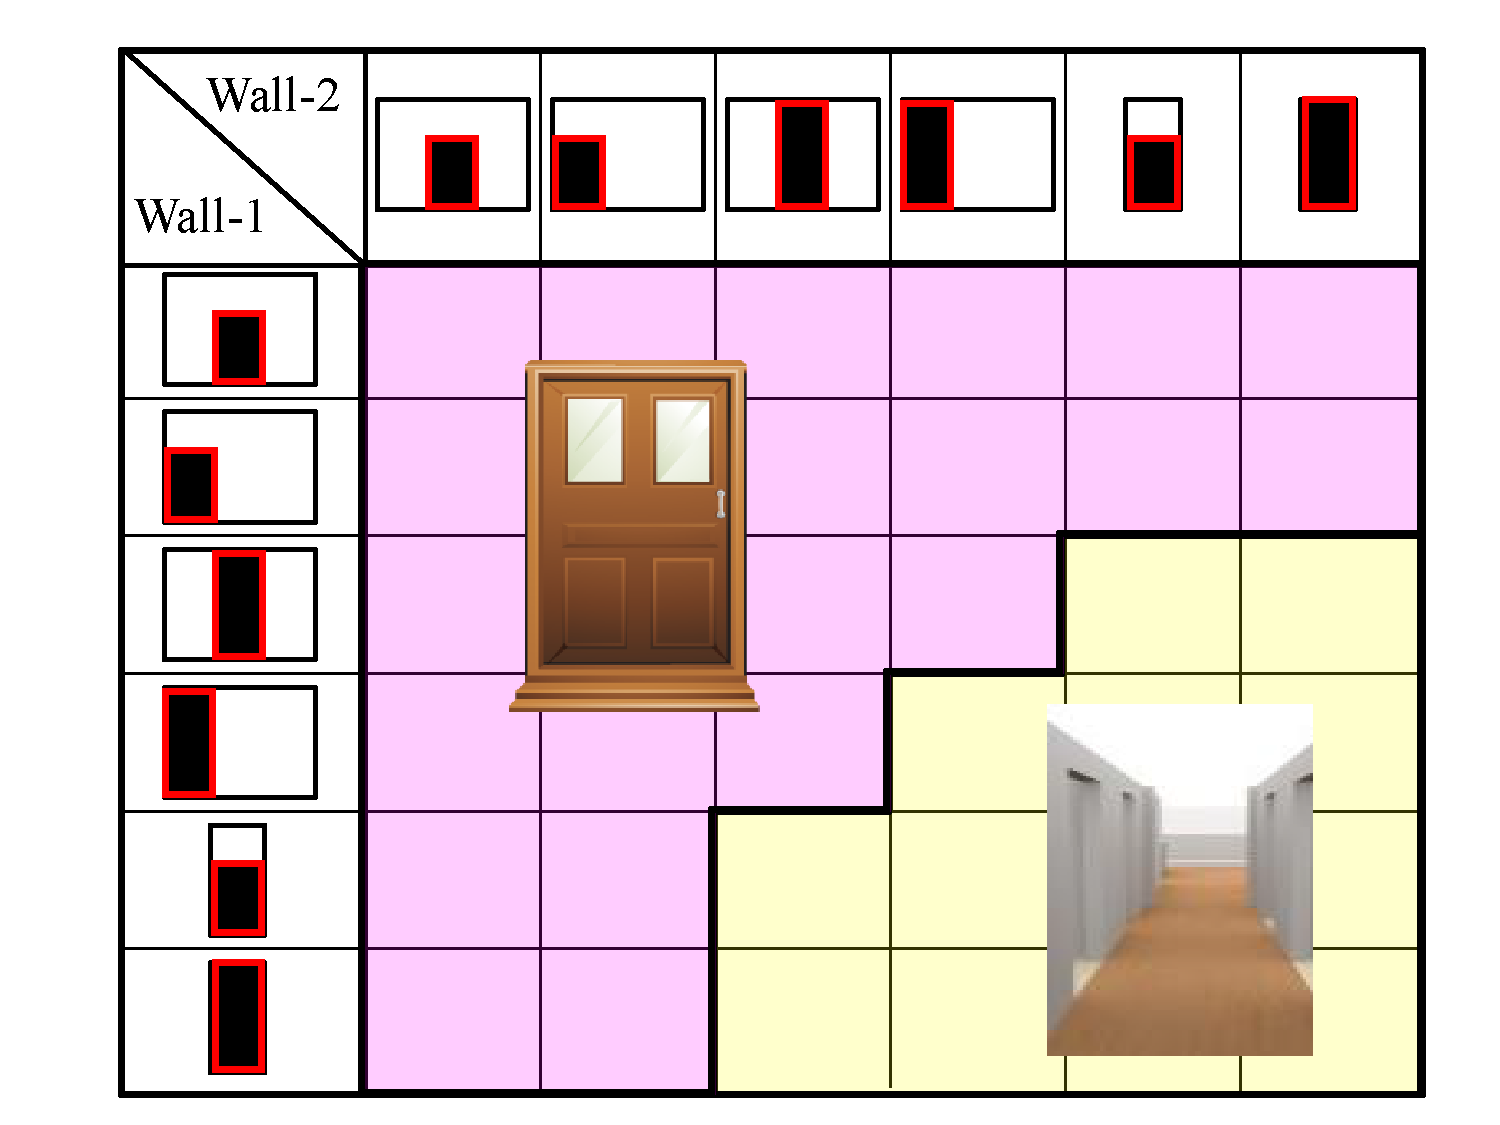
\includegraphics[width=85mm]{../figures/dooranalysis.pdf}
	\end{center}
	\vspace{-0.2cm}
 \caption{Classification table for the room connection types.
 Based on the configuration of the three margins, each wall is
 classified into six types. The combination of the two wall types
 classifies the room connection into either ``door'' (top-left) or
 ``merge'' (bottom-right).
 % Here
 %        we categorize each wall into one of six condition based on the
 %        wing and top distances, and refer the cell that is provided by a
 %        combination of labels of two walls. \yasu{change the icons at
 % the left and the top, which are very confusing.}\yasu{make door and
% open icon better.}}
 } \label{fig:dooranalysis}
	\vspace{-0.25cm}
\end{figure}
This section details in the classification of the room connection, given
the rectangles on the two opposing walls.
%(we should note that $\lambda_1 = 0.01$, and $\lambda_2 = 0.001$ in the
%experiments).
We measure the three margins between the door and the wall boundary in
each wall as in Fig.~\ref{fig:wallprofile}. Depending on the existence
of the margins against some thresholds, each wall is classified into six
different configurations (See Fig.\ref{fig:dooranalysis}). Finally, the
room connection type (either door or merge) is determined as shown in
the table. The thresholds for the horizontal and the vertical margins
are $0.13$m and $0.05 \times \mbox{\{wall height\}}$, respectively.


% Each of the two walls are classified into three types: 

% Then, we assign two types of labels to each wall based on the distances
% mentioned above. The first label is the wing label which has three
% conditions; (w-1) two-side wing: $L_W\geq \alpha_1, R_W \geq \alpha$,
% (w-2) one-side wing: $L_W\geq \alpha_1, R_W < \alpha$ or $R_W\geq
% \alpha_1, L_W < \alpha$, (w-3) $L_W < \alpha_1, R_W < \alpha$. The
% second label is the top label which has two conditions; (t-1) $T_W \geq
% \beta$, (t-2) $T_W < \beta$.

% Using the combination of those two labels (The total combination of
% two-labels are six ($3\times2$)), we refer the classification
% table~\Fref{fig:dooranalysis} to recover the door connection type. Here
% we use $\alpha_1 = 0.13$ m and $\alpha_2 = 0.05\times(WallHeight)$ in
% our experiments.


%
% The classification table evaluates the standard door geometry, where the
% door connection generally has wings and the top, but open connection
% does not have them, however the actually connection is more complex than
% that due to the complex ceiling geometry or noises on the point
% cloud. In those cases, we observed that we often mis-classify the open
% connection as a door. For avoiding mis-classification, we also consider
% the statistics of the dataset. Assuming that the door size of the same
% building are close with each other, we consider the too large door as a
% mis-classified open connection. And if the width of the rectangle is
% larger than min(doorwidth) + std(doorsize(:,1)), we classify as the open
% connection instead of the door connection.




\section{Algorithmic details}
The section provides algorithmic details that were not covered in the
main paper.

\subsection{Pre-processing}

Points cloud acquired by multiple depth sensors are generally corrupted
by mirrors, windows, reflective objects, and calibration errors, which
may affect the quality of reconstruction. Therefore, we first remove
noisy 3D points by the following two filters.

\mysubsubsection{Intensity-based filtering}
%for window and reflective objects}
Most depth sensors emit the infrared
light and record the pixel-wise intensity of the reflected light. At the
presence of windows or reflective objects, corresponding intensity
values become low. Therefore, we remove points if the intensity values
are less than $\mu_I - \sigma_I$, where $\mu_I$ and $\sigma_I$ are the
mean and the standard deviation of the intensities in that image.

\mysubsubsection{Connected-component filtering} The intensity thresholding
is not effective against the mirrors, however these 3D points tend to be
highly isolated. We compute the binary
mask in exactly the same way as the computation of $\Psi$ in the room
segmentation, but this time, based only on one panorama depth image. We
simply keep the largest connected component and discard 3D points that
project outside. This filtering is conducted for each panorama depth image.
% On the other hand we observed that mirrored points cloud could be
% detected by looking at the 2-D projection of the point cloud. Since the
% vertical viewing angle of a standard depth sensor is relatively small
% (\eg, 57 degrees for Microsoft Kinect), the floor points between mirror
% surface and mirrored points are missing (See
% \Fref{fig:noiseremoval}). Based on the observation, we project the all
% 2-D points onto the Manhattan $X-Y$ plane, and remove the significantly
% isolated points on the 2-D plane.
%
This criteria may not completely remove the mirror points, but
is enough for our algorithm to suppress further noise in the
reconstruction process.


% \begin{figure}[!t]
% 	\begin{center}
% 		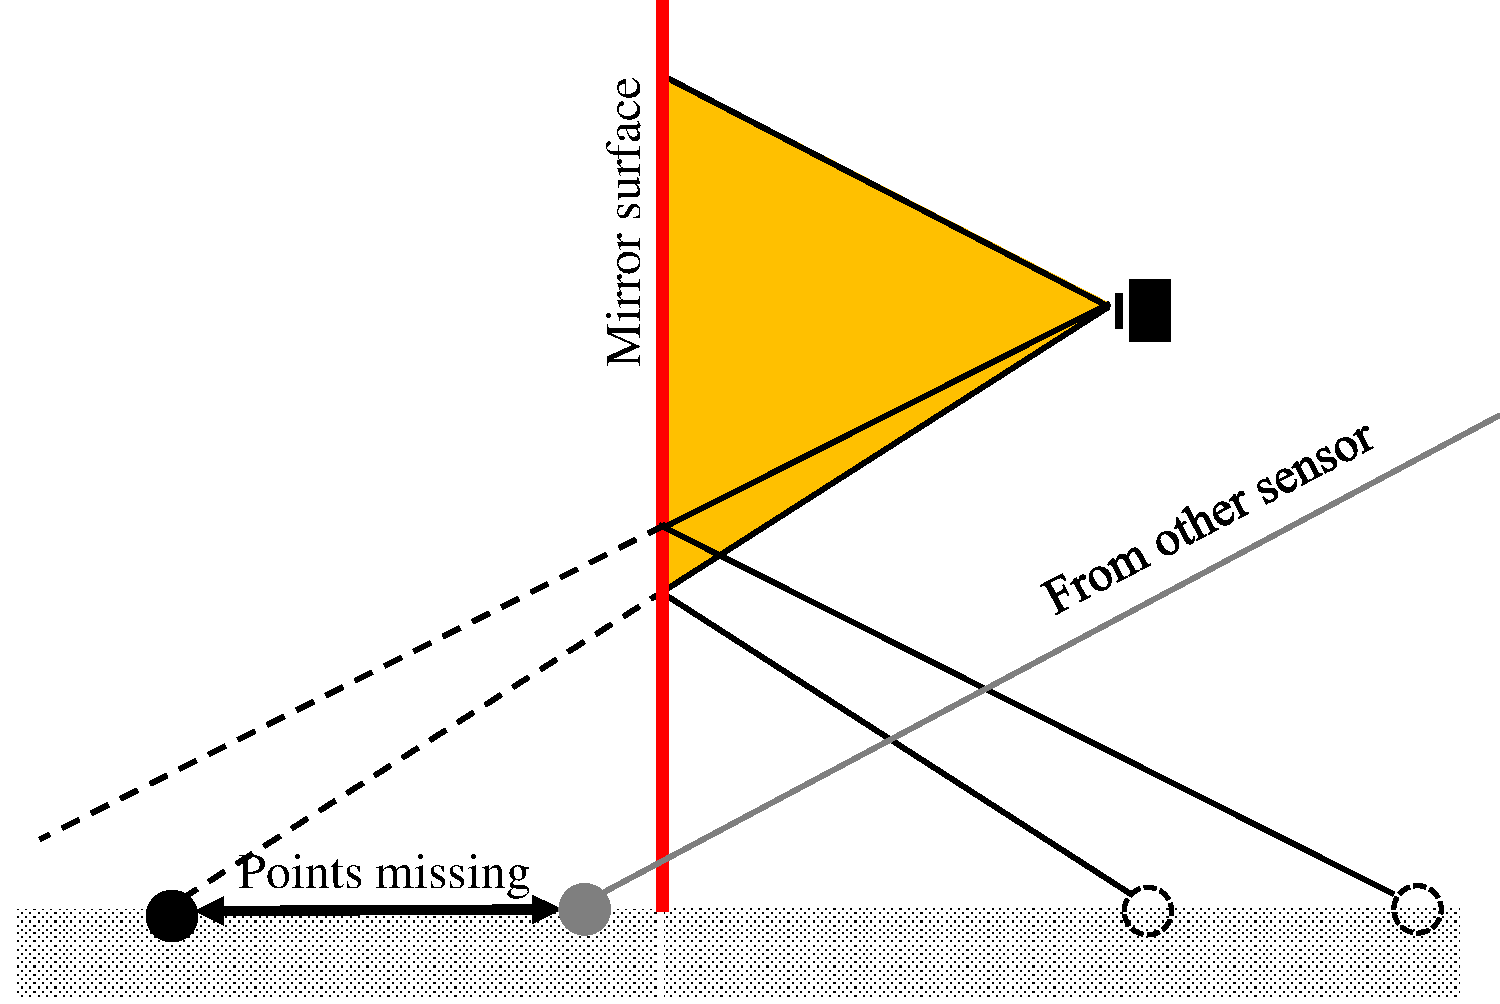
\includegraphics[width=85mm]{../figures/noiseremoval.pdf}
% 	\end{center}
% 	\vspace{-0.2cm}
% 	\caption{When the point is reflected on the mirror, generally the missing region is observed between mirror surface and the mirrored points.}  \label{fig:noiseremoval}
% 	\vspace{-0.25cm}
% \end{figure}


\subsection{Room reconstruction}
The room reconstruction algorithm is based on the previous
work~\cite{floorplan_14}, while we make an adjustment to the {\em core
free-space region} extraction algorithm. The core free-space is computed
as the space with very high free-space evidence, where the room boundary
should not pass through. This caused a problem in our setting. Our
input comes from a depth sensor, while their input is an MVS
point-cloud. A depth sensor generates very strong outliers near the
windows, and their core free-space region often crosses walls through the
windows.

Our approach is to restrict the core free-space region to be an axis
aligned rectangle. More specifically, we find the axis-aligned rectangle
that fits inside the domain $\Psi$ and minimizes the following objective
function:
\begin{eqnarray*}
 max(H, W) + \eta H W,
\end{eqnarray*}
where $H$ and $W$ denote the width and height of the rectangle, and
$\eta=0.001$ is used in our experiments.  This objective has an effect
to maximize the rectangle while keeping its aspect ratio close to 1. We
find the solution via the exhaustive search.


% Here we describe the details of our room reconstruction grammer that we
% omitted due to the space limit. The major framework of the algorithm is
% same with the previous work~\cite{Cabral2014}, that contains (a)
% core-freespace generation, (b) start-end line extraction, (c) path
% optimization. However, we take slightly different strategies since the
% original algorithm is optimized for single room room, while we tackle
% the building scale reconstruction.

% \mysubsubsection{Initialization} The input of the
% algorithm~\cite{Cabral2014} is wall evidence and free-space evidence,
% where wall evidence is the point evidence generated from the points
% whose normal is either of ${X,-X,Y,-Y}$. Here we define wall-evidence
% and free-space evidence {\it independently} for each room
% reconstruction. First, we divide frees-space into regions based on the
% structured graph. While our room node does not always cover the entire
% region as shown in third row of Fig. 2 in the main manuscript, we
% spatially propagate labels so that every pixel in the fees-space
% evidence has a label that corresponds to the room index on the
% graph. And then we compute the wall and free-space evidence where pixels
% in the region of the target room.  (I will add fig later). This per-room
% evidences make the algorithm quite robust and computation of the path
% much more efficient.


% The core free-space region as a high free-space evidence as defined
% in~\cite{Cabral2014} is problematic for our condition since the
% frees-space generally brides different room (even though we define the
% local evidence) and per-room reconstruction becomes impossible.

% Therefore, we instead compute the core free-space by solving following
% optimization problem,
% \begin{equation}
% \min_{\Omega \in RectSet} max(H_{\Omega}, W_{\Omega}) + \gamma H_{\Omega}W_{\Omega}.
% \end{equation}
% where ${RectSet}$ is a collection of rectangles that are completely
% included in the non-zero regions of local free-space evidence and
% $H_\Omega$ and $W_\Omega$ are height and width of a rectangle
% proposal. This equation maximizes the size of core-freespace
% region($\Omega$) while preventing the shape of the evidence from being
% too elongated. This equation quantifies the reasonable observation that
% the room shape is generally convex except for the door part and details
% on the wall such as windows.

% \mysubsubsection{Shortest path reconstruction} Given three information
% (a) the local evidence, (b) the core free-space, and (c) the start-end
% line (in the same manner with~\cite{Cabral2014}), then we reconstruct
% the shortest path that minimize the total edge.

% While \cite{Cabral2014} prevents the path go through the high free-space
% evidence by the hard constraint (core free-space), we instead avoid the
% path to go thorough the high free-space evidence as a penalty in the
% edge cost:
% \begin{eqnarray}
% e_{\rho} = \frac{1}{1+\beta}\sum_{k=1}^{|\rho|}{\left(1-P_W(c_k)+ \beta(c_k) F(c_k)\right)}\nonumber\\
% +\omega,\label{eq:edgecost}
% \end{eqnarray}
% where $c_k$ is a cell that is included in on edge $\rho$. $\omega$ is a
% constant mode-complexity penalty, which biases our solution towards
% paths with less edges ($\omega = 7$ in our experiments). $\beta$ is a
% weight that balances the contribution the free-space evidence and wall
% evidence ($\beta(c_k) = 1$ if $P_W(c_k) = 0$ and $\beta(c_k) = 1.5$ if
% $P_W(c_k) > 0$ in our experiments. We vary $\beta$ for strongly
% penalizing the path that go through the empty cell).

% The optimization is achieved in the same manner with~\cite{Cabral2014}
% and the resultant shortest path is composed of the multiple edges:
% $\rho_1, \rho_2, \cdots, \rho_m$, we define them as the |{\it wall
% elements} in our structured graph.

\subsection{Wall/ceiling detail reconstruction}

% \begin{figure}[!t]
% 	\begin{center}
% 		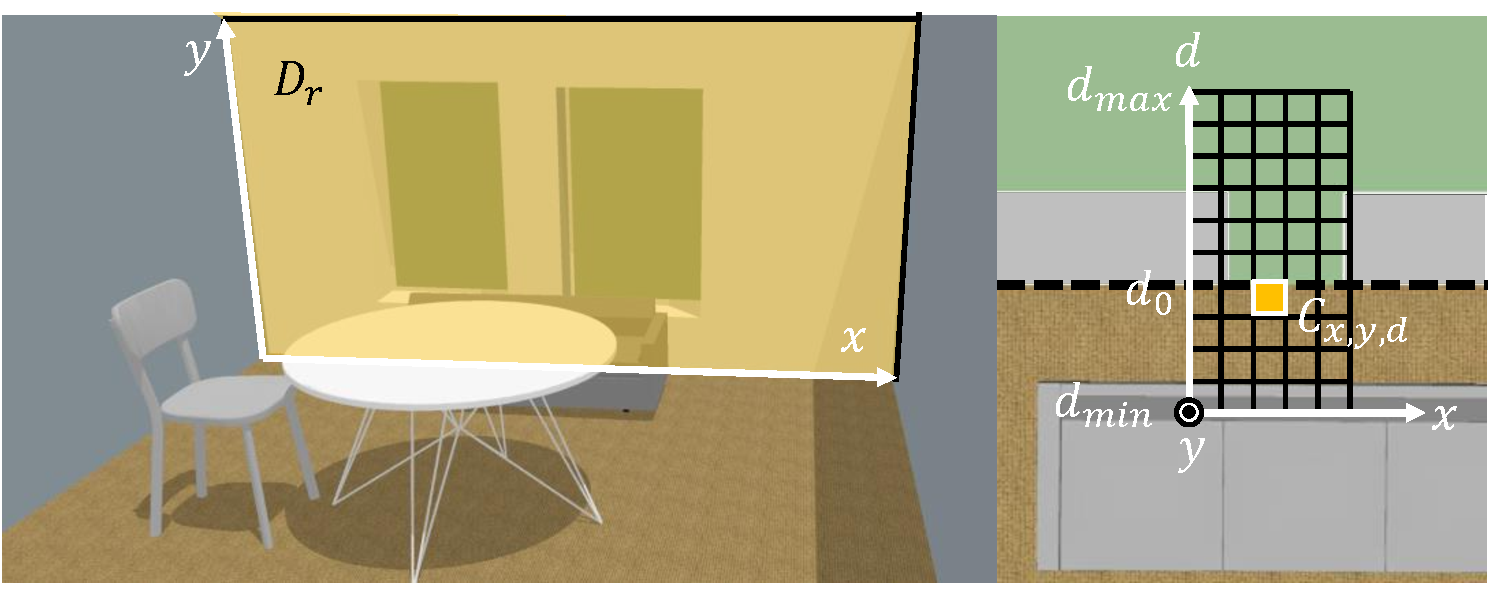
\includegraphics[width=85mm]{../figures/detailreconstruction.pdf}
% 	\end{center}
% 	\vspace{-0.2cm}
% 	\caption{Given a target wall, we construct the costvolume aligned with the Manhattan-World directions. The offset-map is then computed on the $x$-$y$ plane by aggregating the cost via MRF optimization. }  \label{fig:detailreconstruction}
% 	\vspace{-0.25cm}
% \end{figure}
% In this section, we describe the initialization of the offset map
% ($D_r$) in our main manuscript.

% We firstly define the cost-volume that is parallel to the Manhattan
% directions whose inbound and outbound range from the base plane is
% $d_{min}$ and $d_{max}$, respectively (See
% \Fref{fig:detailreconstruction}).

The initial offset-map in the wall/ceiling detail reconstruction is
obtained by a simple 2D MRF with unary and pairwise terms:
\begin{eqnarray*}
 E = \sum_p E_d(d_p) + \lambda \sum_{\{p,q\} \in \mathcal{N}} E_s(d_p, d_q).
\end{eqnarray*}
$p$ and $q$ denote pixels, while $d_p$ is the estimated offset-value at
pixel p.  The pairwise term $E_s$ follows a $Potts$ model where $\lambda
= 0.01$ is used in our experiments. The unary term $E_d$ is defined
as
\begin{equation*}
E_d(d_p) = -P(p, d_p)\left(\sum_{d=d_p^{min}}^{d_p} F(p, d)\right). \label{eq:costdetail}
\end{equation*}
$P(p, d_p)$ and $F(p, d_p)$ denote the point and free-space evidence at
pixel $p$ and offset $d_p$, respectively. Intuitively, the cost becomes
smaller if the point evidence and the accumulation of the free-space
evidence are large. The valid depth range of a pixel $[d_p^{min},
d_p^{max}]$ is computed from the domain $\Psi$ for the room segmentation
in the top-down view. More concretely, we simply cast rays in the two
opposing directions orthogonal to the wall, and obtain the first
intersection with the boundary of $\Psi$ each. Finally, we get the
intersection with the range $[-2\mbox{m}, 2\mbox{m}]$ to avoid unnecessarily large
search space.



% where $P$ and $F$ are the point/free-space evidence, and $x$, $y$ and $d$ are the indices of a cell with regard to wall ($x-y$) and depth ($d$) directions, respectively. 

% Intuitively, if we cast a ray from $d=d_{min}$ to the outgoing direction
% that is perpendicular to the wall, the cost is minimized at the out-most
% intersection to the surface. However, the input point cloud is often
% sparse near the wall and it happens that the ray from the viewpoint does
% not intersect with any points (\ie, the cost for any off-set values is
% zero). For tackling this issue, we simply propagate the information from
% the neighborhood pixels by solving the MRF-optimization problem as
% \begin{equation}
% D_0 = \argmin_{\textbf{d}}{\sum_{p}Cost(p,l) + \lambda \sum_p{\sum_{q\in N(p)}}{Potts(l_p, l_q)}},
% \end{equation}
% where $p$ is an index on the $x-y$ plane, $Potts$ is the potts penalty
% that gives zero if two labels are same and otherwise one ($\lambda =
% 0.01$ in our experiment). Then, the offset-map is used as an initial
% values of $D_r$ as we have already mentioned in the main manuscript.




\section{Application Details}

This section presents the details of our applications demonstrated in
the main paper and the supplementary video.

\subsection{Floorplan generation}

Figures~\ref{fig:room_recog} and \ref{fig:room_recog1} illustrate the
results of the room annotation experiments. The room annotation did not
work well with the full panorama images, and we render $400\times 300$
standard perspective images with the horizontal field of view of $90$
degrees. The results heavily depend on the choice of the viewing
directions and we experimented the four algorithms in an increasing
order of accuracy. The first algorithm picks the panorama closest to the
room center, generates six uniformly overlapping images, and picks the
scene type with the best average score. The second one exploits more
scene information, and uses only one image out of six, in which the
visible room area is the maximum in the top-down view. The third
algorithm uses the second algorithm for all the panoramas inside the
room, and uses the average to pick the best score. The last algorithm
takes the same set of images as the third one, but only uses a single
image, in which the room is the most visible. Surprisingly, this last
algorithm works the best on all the datasets. An observation is that
poorly positioned panoramas tend to yield incorrect results but with
very high confidence. A rather better strategy is to use the best
viewing direction from the best panorama.


  
Figure~\ref{fig:object_recog} shows the object annotation results, which
turn out to be much more challenging than the room annotations, even
with the state-of-the-art object
detectors~\cite{berkeley_object_detection_software}. Our object
annotation has the following three steps. First, object detector is
applied to each panorama image, where two images are generated from each
panorama by shifting the left image boundary by half the image width to
avoid having objects across the image boundary. Object detection results
are simply merged for each panorama. Second, the structure graph is
rasterized into each panorama with a depth testing, while keeping track
of the structural element ID. Lastly, starting from the object detection
with the highest detection score, we identify the object element that
has the most rasterized pixels inside the bounding-box of the object
detection. The process repeats after removing the matched object
detection and the element. We only keep the annotations that are related
to furniture in the indoor scenes (\ie, chair, lamp, table, desk, sofa,
and bookshelf).

%Room annotations are obtained by the state-of-the-art scene recognition
%system~\cite{mit_scene_demo_paper}. Based on the reconstructed 3D
%models, we generate standard perspective images from panoramas. The
%details of this experiment are given in
%Sect.~\ref{section:supple:results} in this supplementary material.


We change the rendering style and shape of object icons depending on the
object recognition results. For example, we have a special icon for
desk, sofa, chair, and a lamp, respectively. The chair and the sofa have
orientations, and we simply orient the icon so that the front side
becomes the closest to the center of the room. Ideally, an image
information should be used to determine the orientations of the
icons. The outlines of the desk and the remaining (unannotated) objects
are computed from the segmented 3D point clouds. After projecting the 3D
points on the X-Y plane, a 2D version of the Marching
Cube~\cite{MarchingCube} algorithm is used to extract the polygon,
followed by a mesh simplification algorithm.

% \hang{icon generation} To show objects in floorplan, we need to get the
% 2D shape of objects from top-down view. For each object, we first
% project all points to x-y plane to get a 2D density map. Notice that to
% suppress noise on the object boundaries and get rectangular contours, we
% remove a 5\% margin of confidence map on each side of x and y direction,
% respectively. Then we perform marching square algorithm on the density
% map to get a 2D contour, followed by simplification to reduce vertices
% number and suppress noise. This 2D polygon is then fed into
% triangulation algorithm and transformed to manhattan coordinate system
% and finally rendered in floorplan view.

\subsection{Indoor scene viewer}

Our indoor scene viewer enables seamless visualization across
ground-to-air view-points under various rendering styles. There are a
few important implementation details to be shared.

First, the texture map for the architectural components are computed for
each piecewise planar surface in a single structural element
independently. This is a major advantage enabled by our structure
graph. Due to severe occlusions, we need to inpaint very large texture
holes extensively, and likely misuse wall texture for the floor geometry
with standard techniques, for example. Thanks to the compact mesh
models, piecewise planar surfaces are very large in general, and we
essentially compute the texture for each structural element one by
one. Our approach benefits from both the texture synthesis and the
texture inpainting literature. More concretely, after discretizing the
piecewise planar surface into 2D array of texels, we first project
nearby images to the surface with the depth testing. Due to occlusions,
the projected textures have many holes. Starting from the projected
texture with the least hole pixels, we assign a color to each texel, and
repeat for all the projected textures. We then use a classical texture
synthesis algorithm~\cite{efros1999texture} to synthesize texture for
the hole pixels, while fixing the colors of the non-hole
pixels. Poisson-blending~\cite{perez2003poisson} is finally used to
smooth our texture edges. Note that we also tried an off-the-shelf
texture inpainting tool on PhotoShop (\ie, content-aware fill) to fill
holes, but their produced results were very poor.

Second, the structure graph enables us to render back-facing structures
effectively. First, we can simply ignore ceiling elements, which is not
easy for a polygon-soup mesh model. As shown in
Figs.~\ref{fig:comp_mesh0} and \ref{fig:comp_mesh1},
simple back-face culling leaves numerous small triangle pieces in the
views. In general, our system can render back-facing structural element
as opaque, culled, or translucent. Note that this rendering style is
enforced at the level of structural elements (\eg., a wall), as opposed
to triangles, yielding effective visualize effects without artifacts.

Lastly, the viewer enables a quick room-to-room ground-based
navigation. We compute a path connecting the camera center locations by
a simple shortest path algorithm with the visibility testing in real time.

% \subsection{Inverse-CAD}

\subsection{Tunable reconstruction}

A user specifies the maximum number of polygons allowed for an entire
scene, a room, or a wall. Each number simply puts a constraint at the
corresponding node in a structure graph. Our pruning algorithm is simple
and greedy. Starting from the bottom of the tree, we identify either a
wall, a room, or a scene node that violates this constraint. Then, we
find the set of nodes that can be dropped below the node and has the
fewest number of polygons. We drop the nodes and repeat the process
until all the constraints are satisfied. In the worse case, when the
numbers are tight, the system might drop entire rooms.






% Note that we do not prevent intersections with geometries at the other
% nodes in this step, although it is not difficult to do so (infinite data
% cost for prohibited depth values). Our observation is that the
% topological consistency is crucial for high-end graphics or InverseCAD
% applications. However, a small amount of mesh self-intersections did not
% cause problems in our applications as demonstrated in
% Sect.~\ref{section:applications}



%\clearpage
{\small
	\bibliographystyle{ieee}
	\bibliography{egbib,furukawa}
}
\end{document}
